\documentclass[../Main.tex]{subfiles}
\begin{document}

\subsection{Results}


\subsection{Mobile application}
The final result of a project is mobile application which allows users to pick any photo
and then apply it as a filter in real-time video. Figure \ref{fig:app-results} presents screenshots taken from style transfer screen of an application.

\setlength{\tabcolsep}{0.5pt}
\renewcommand{\arraystretch}{0.2}
\begin{figure}[H]
\centering
\begin{tabular}{cccccc}
&
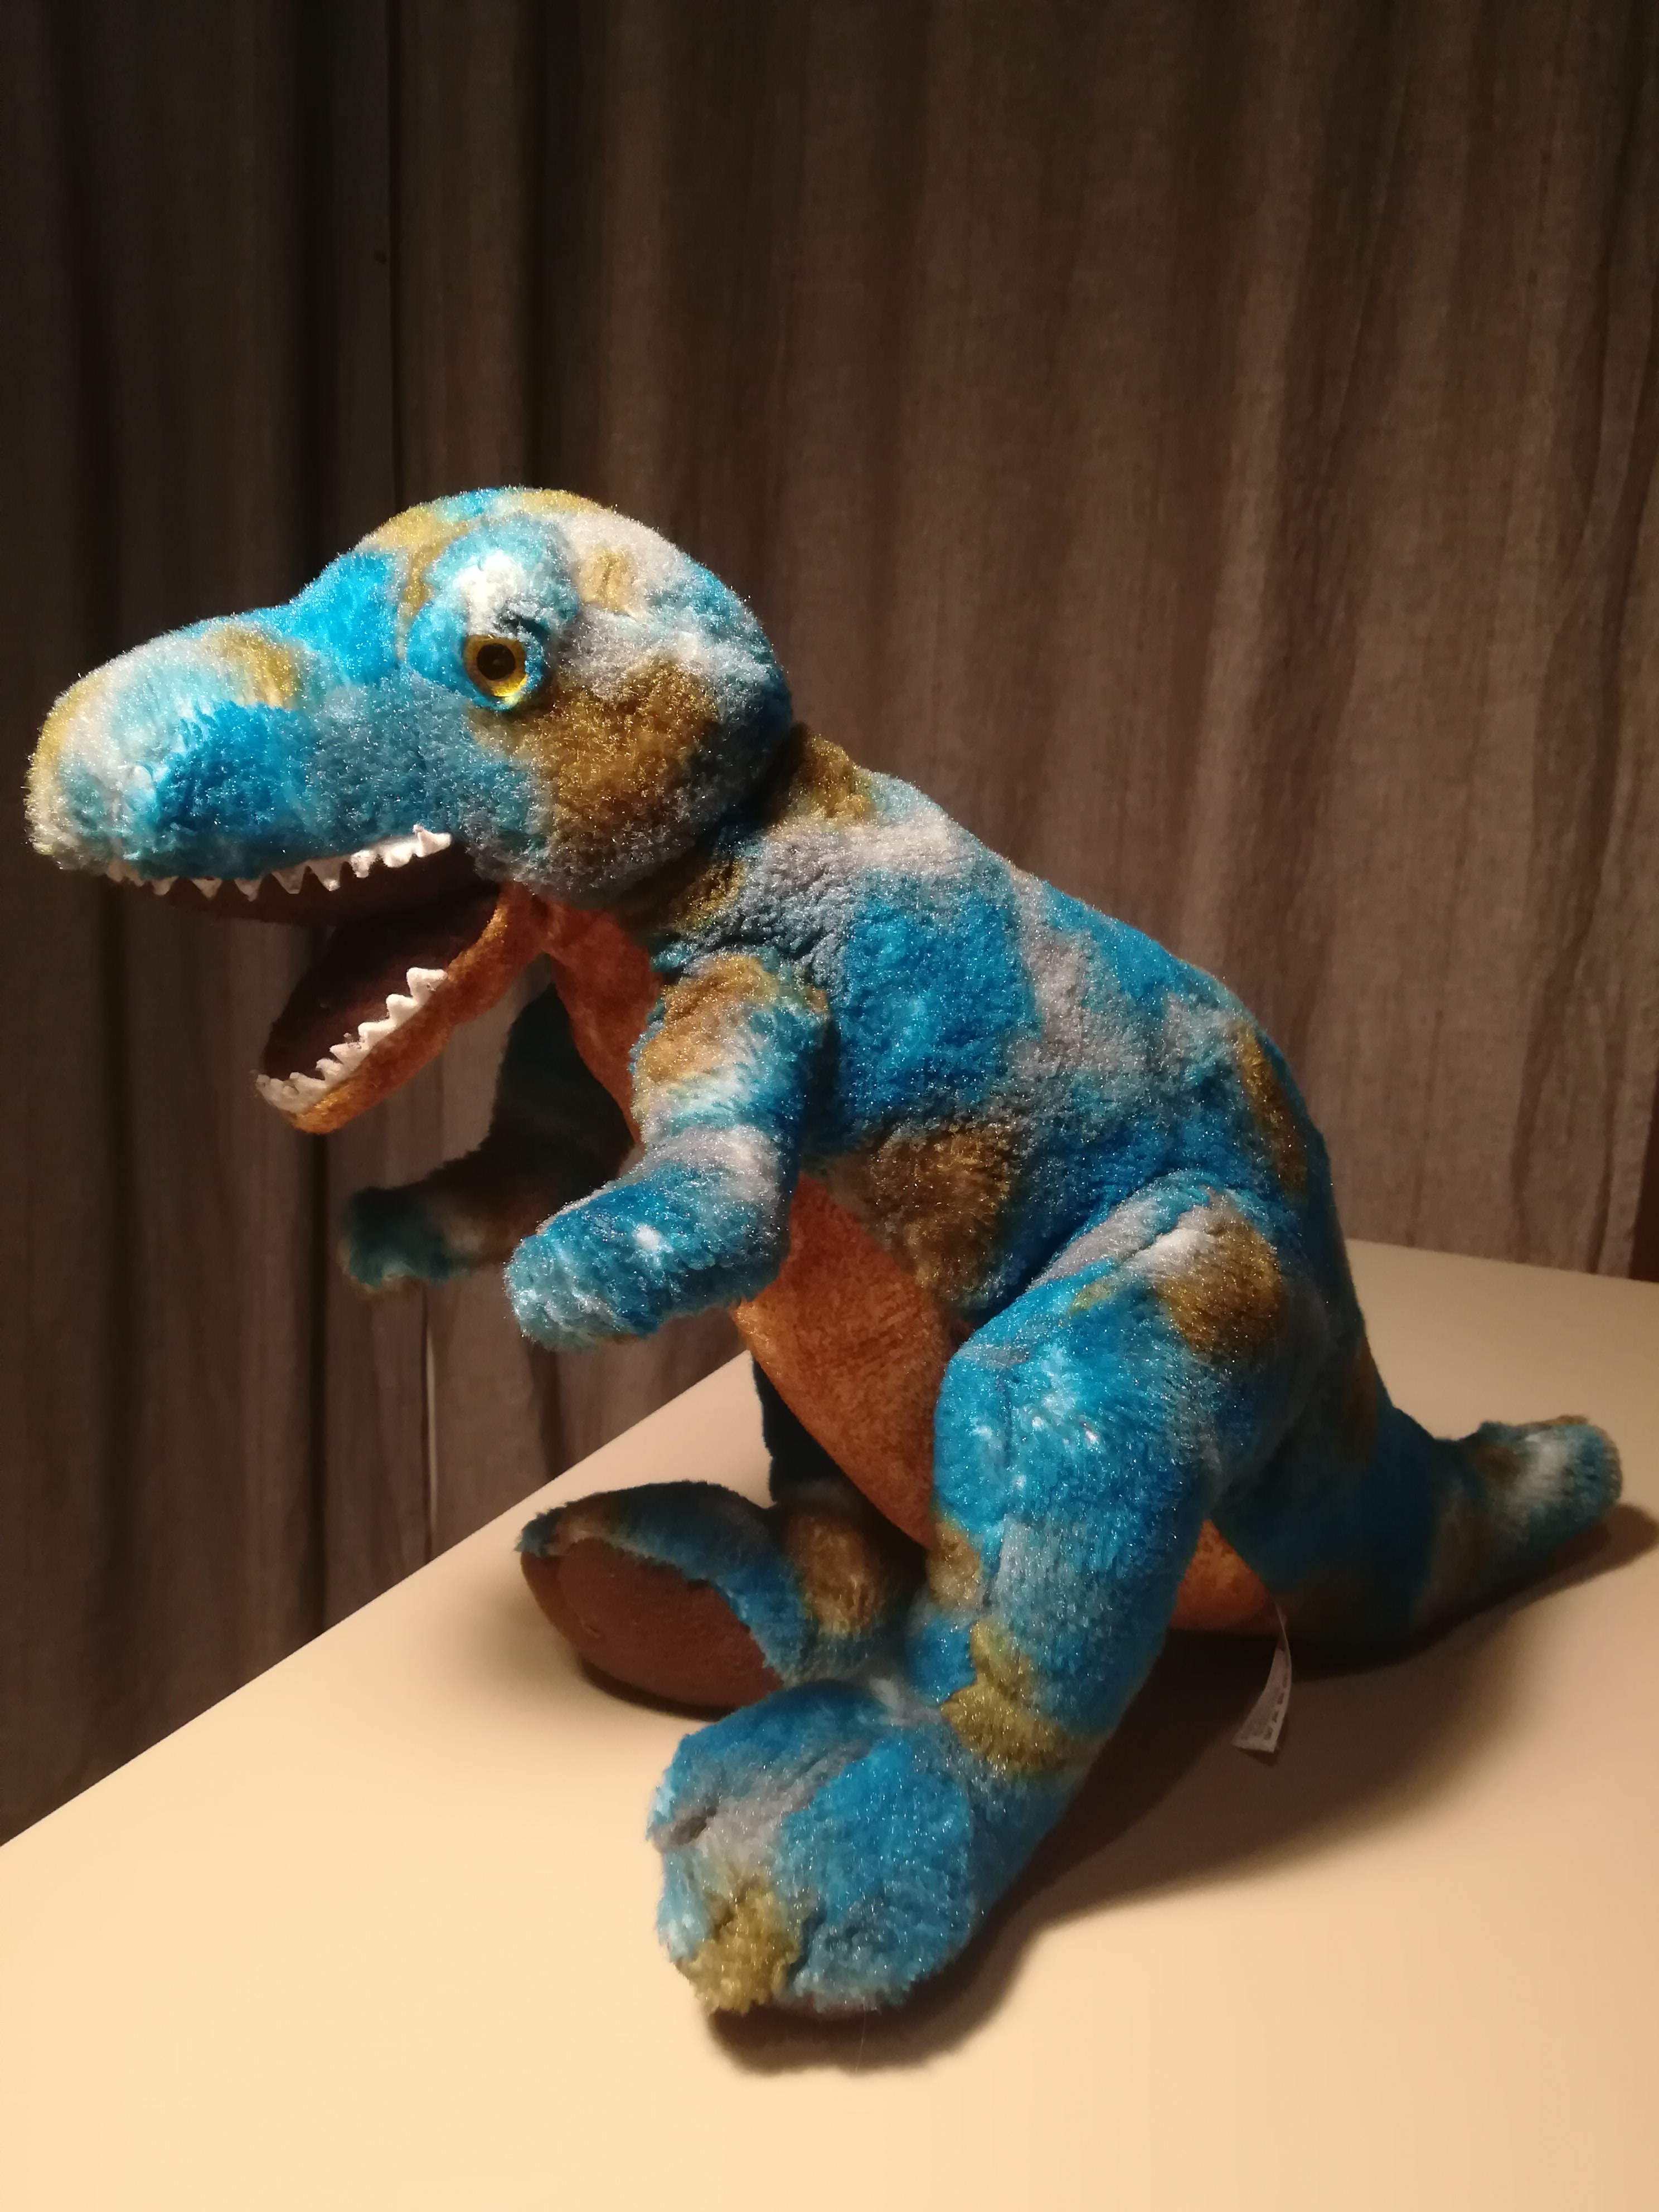
\includegraphics[width = 0.13\linewidth]{Images/app_photos/dino/norm.jpg} &
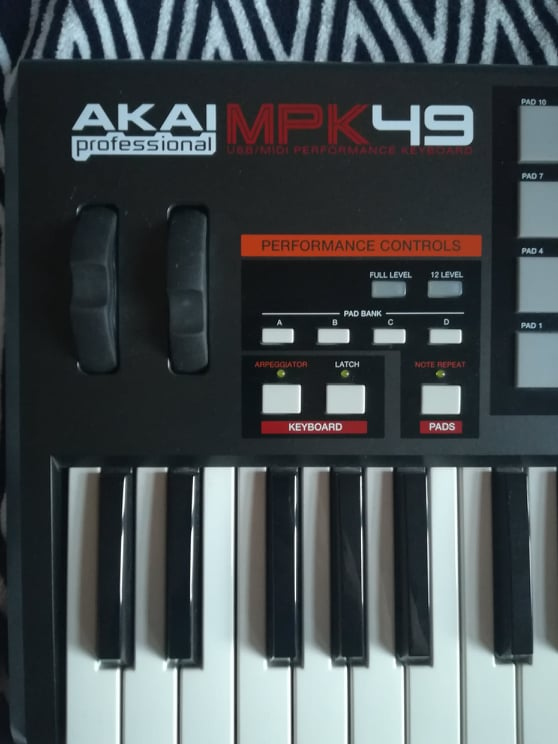
\includegraphics[width = 0.13\linewidth]{Images/app_photos/akai/norm2.jpg} &

\includegraphics[width = 0.13\linewidth]{Images/app_photos/me/norm.jpg} &
\includegraphics[width = 0.13\linewidth]{Images/app_photos/kamienica/norm.jpg} &
\includegraphics[width = 0.13\linewidth]{Images/app_photos/ulica/norm.jpg} \\

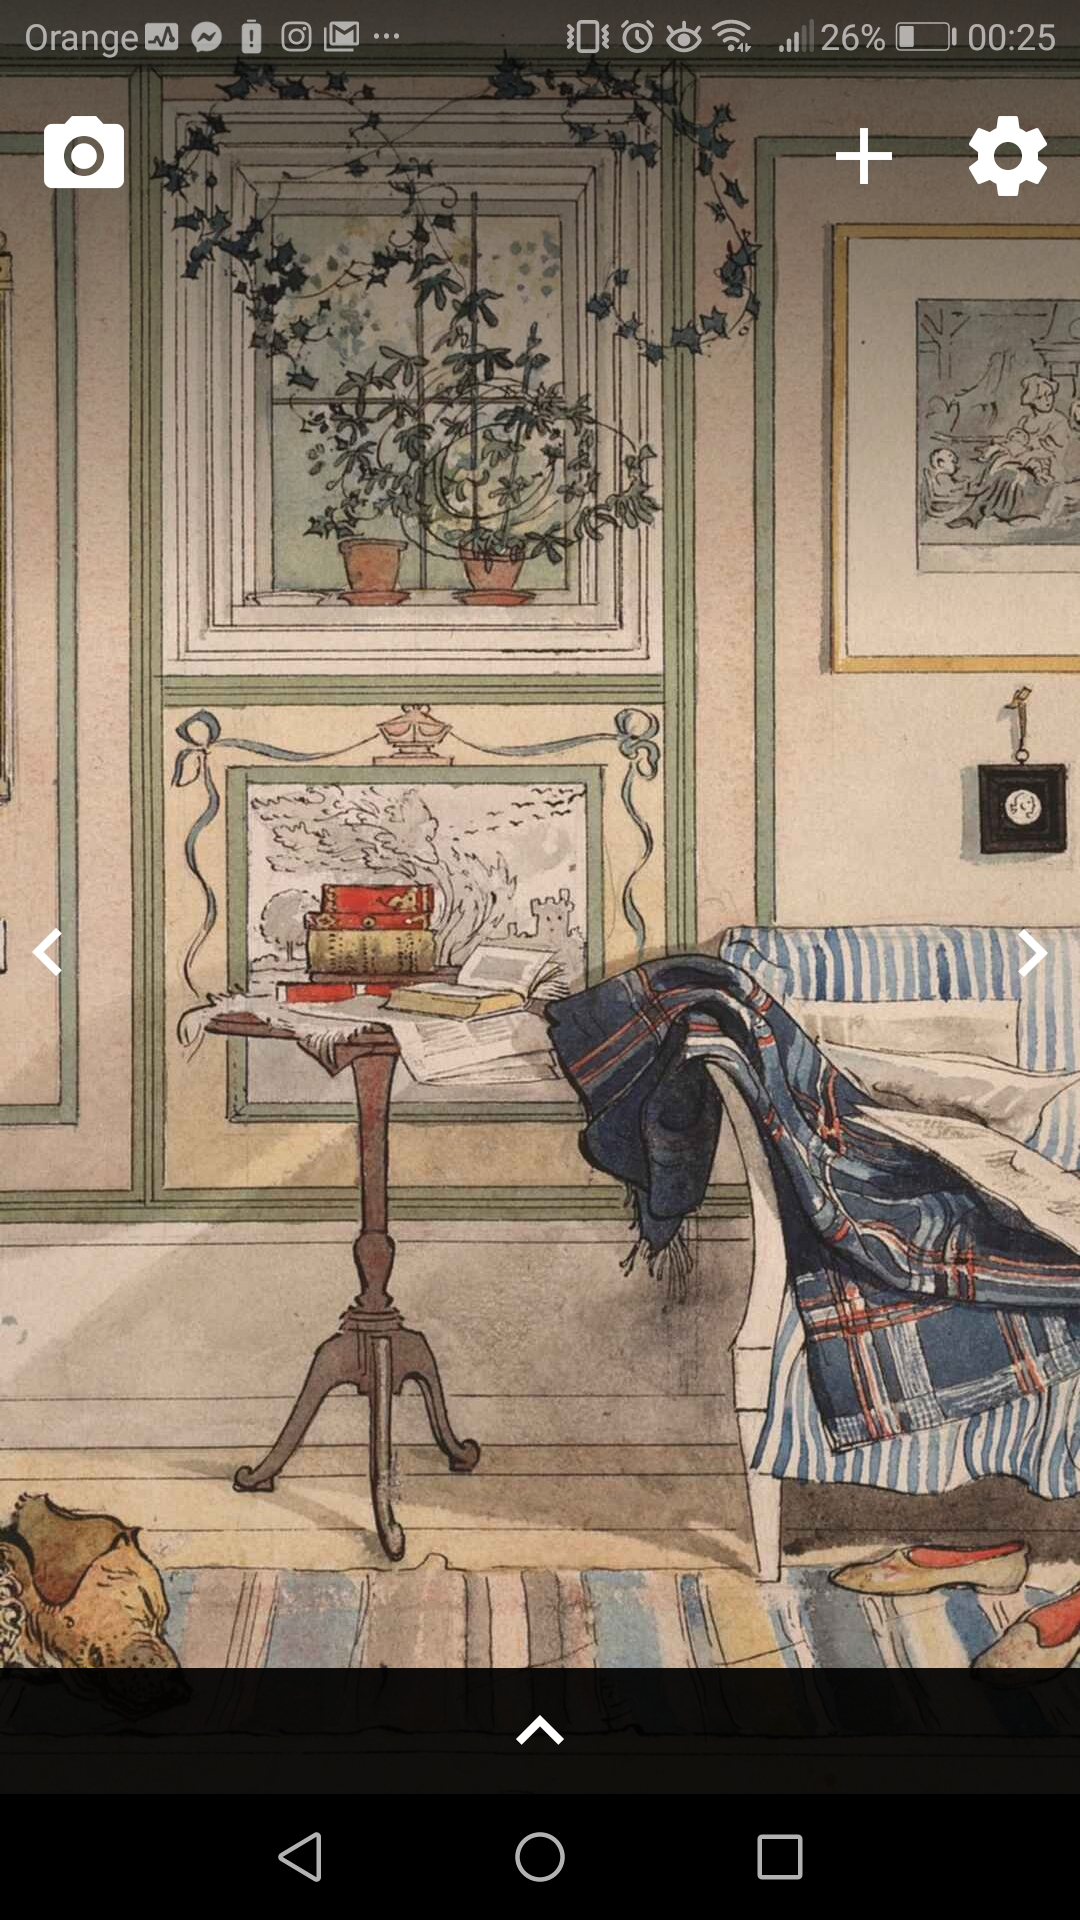
\includegraphics[width = 0.13\linewidth]{Images/app_photos/filters/salon.jpg} &
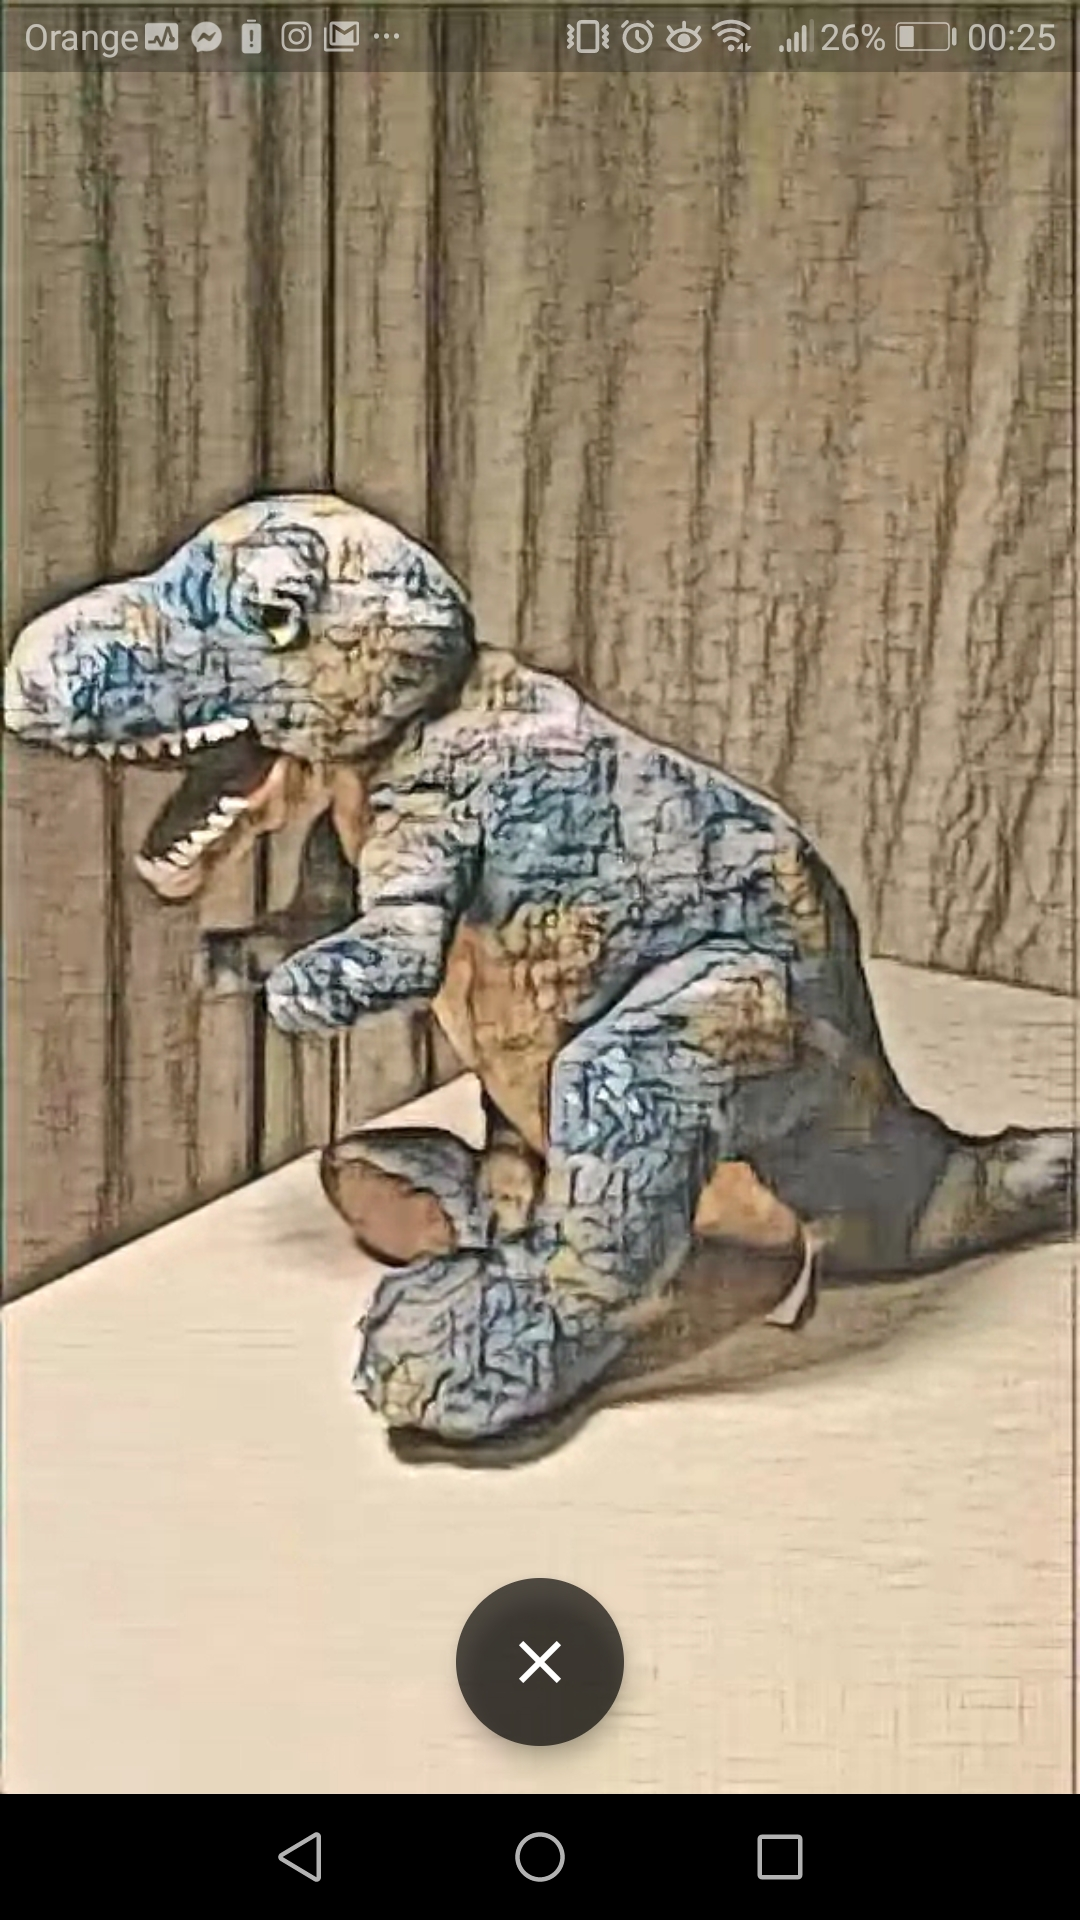
\includegraphics[width = 0.13\linewidth]{Images/app_photos/dino/salon.jpg} &
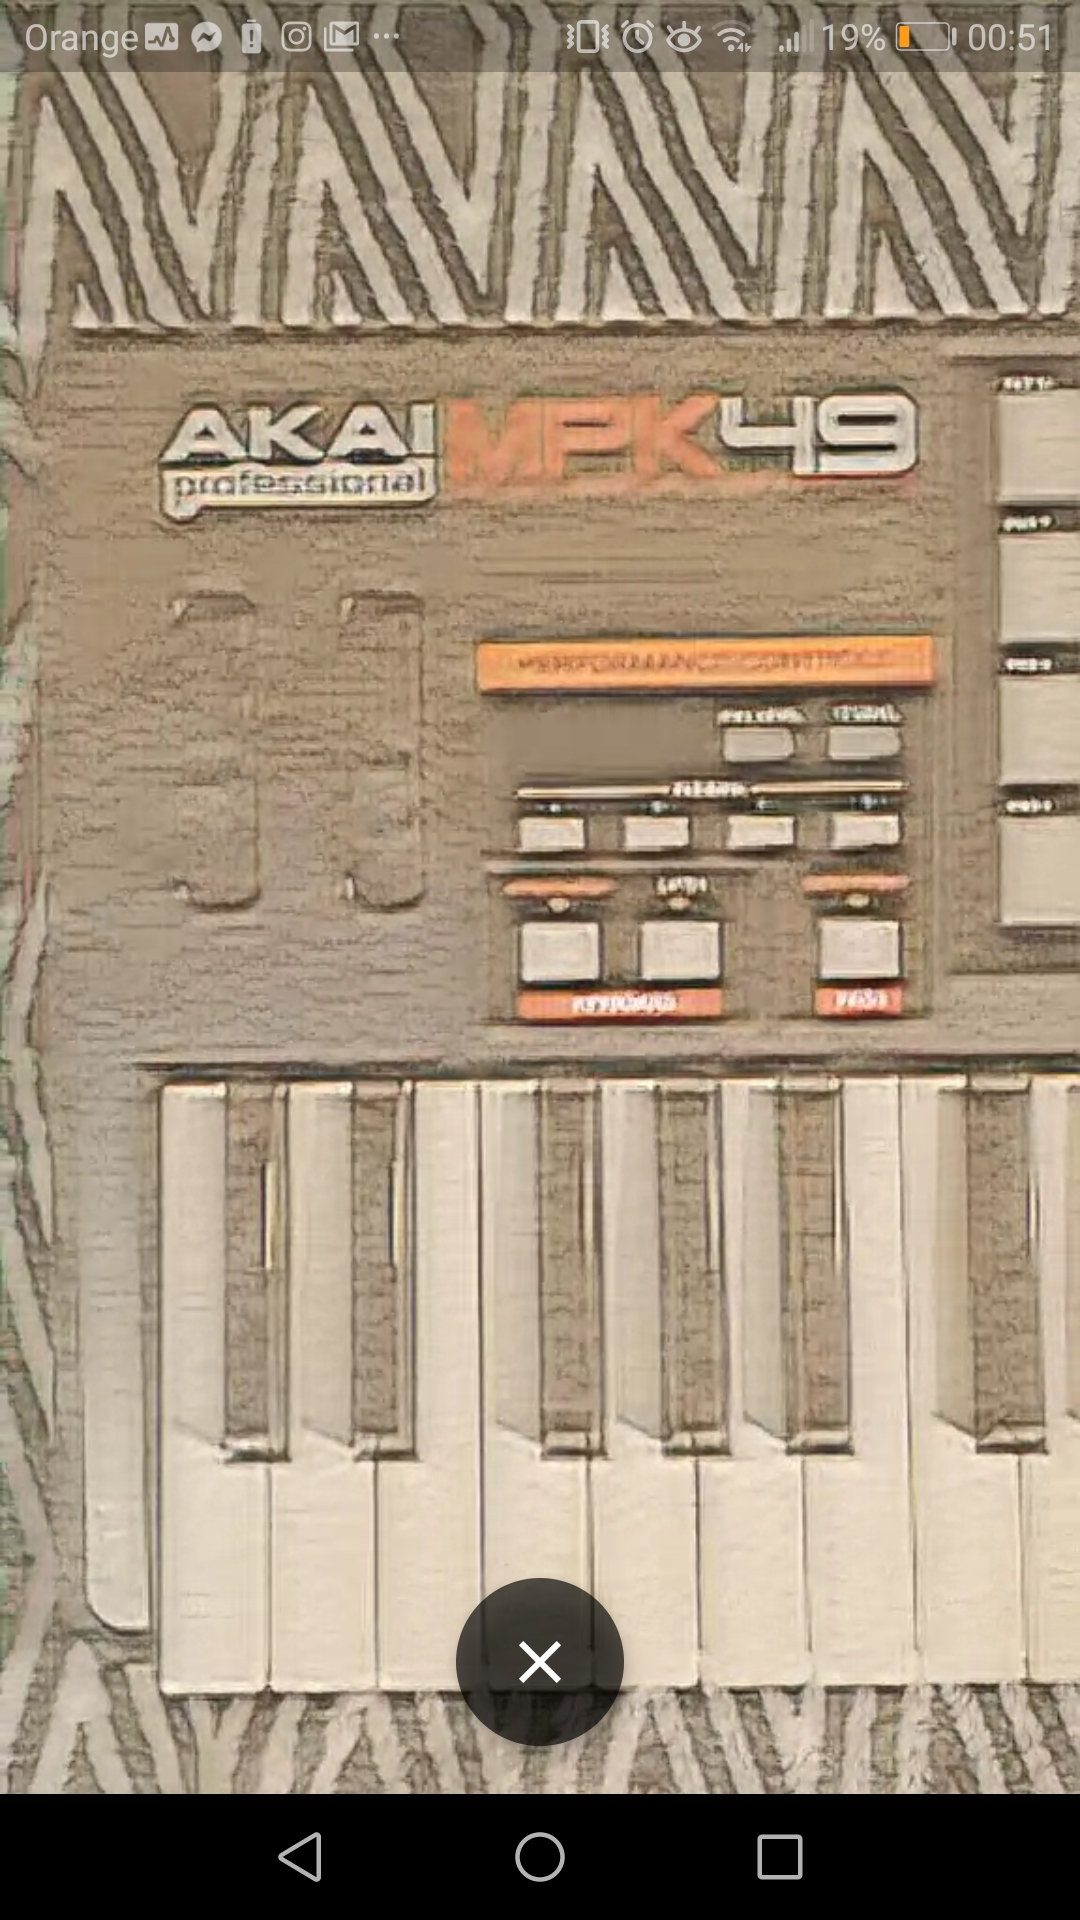
\includegraphics[width = 0.13\linewidth]{Images/app_photos/akai/salon.jpg} &
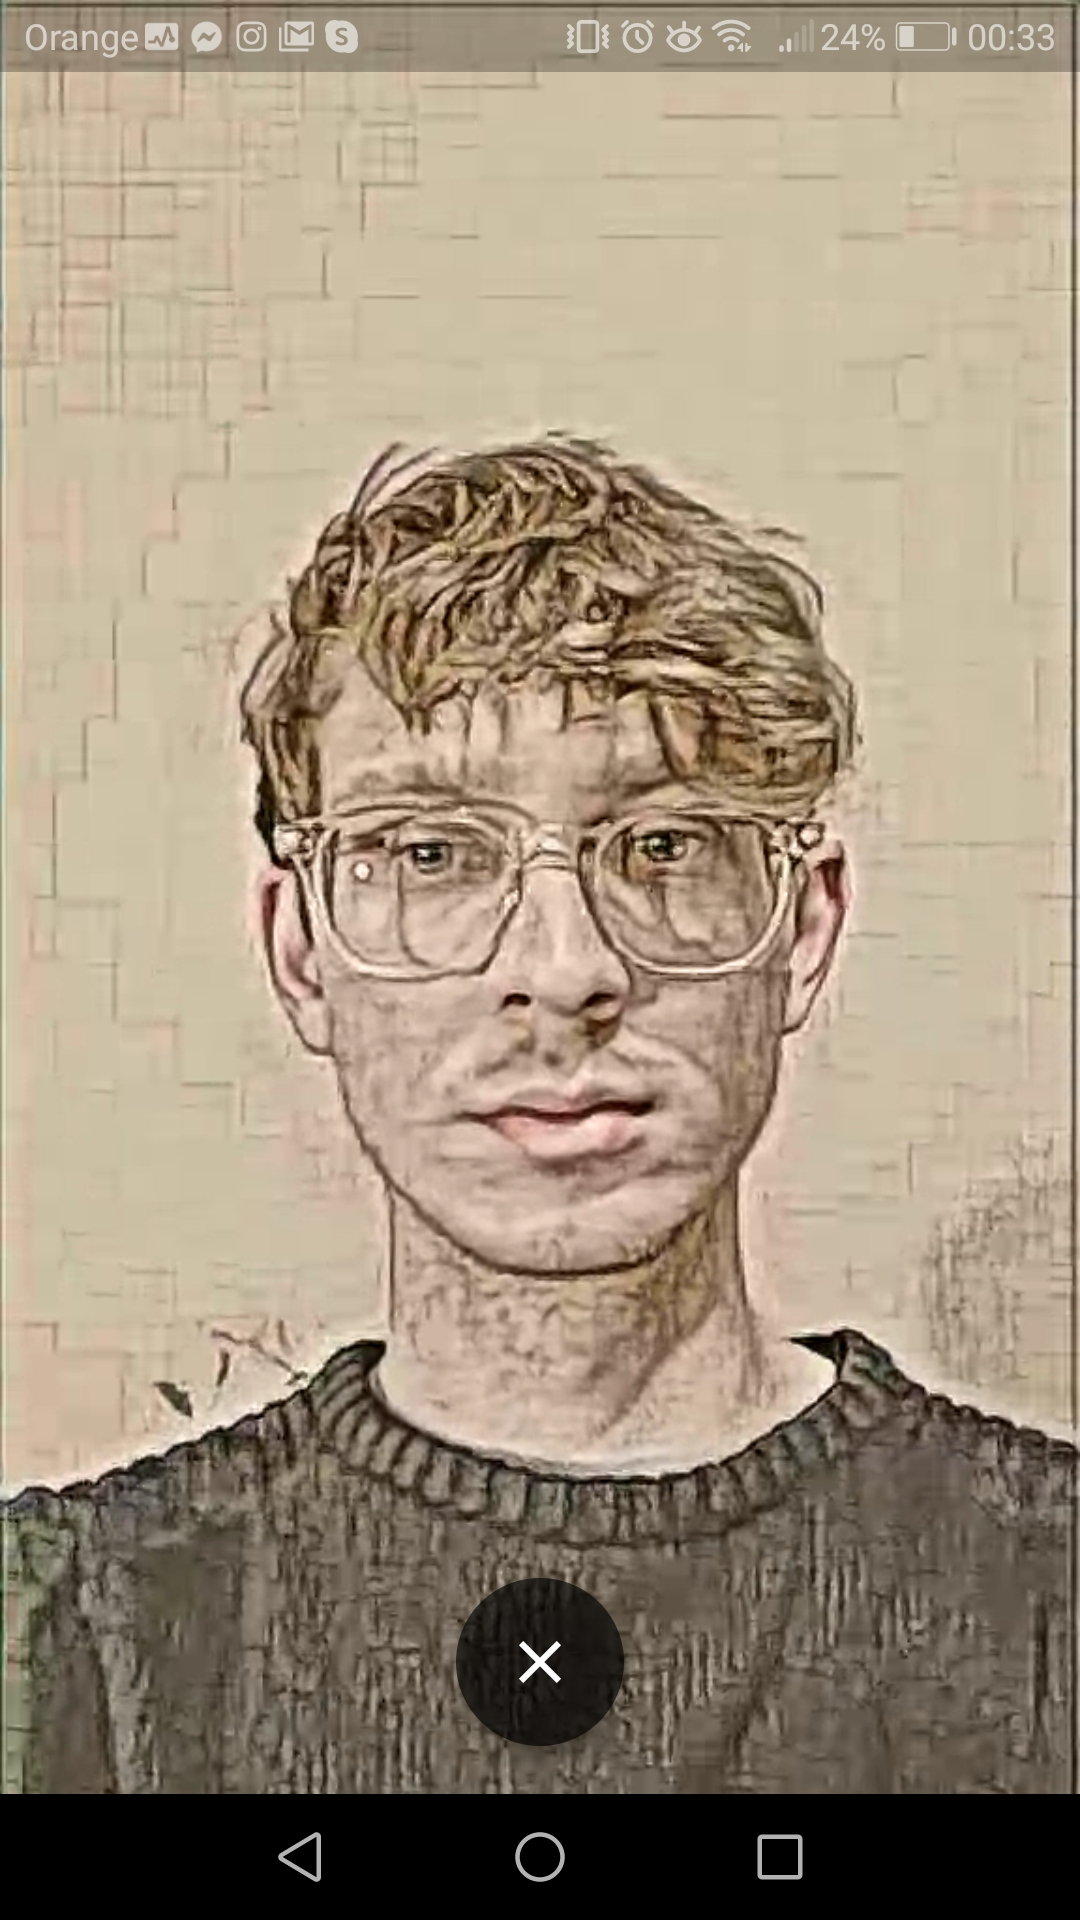
\includegraphics[width = 0.13\linewidth]{Images/app_photos/me/salon.jpg} &
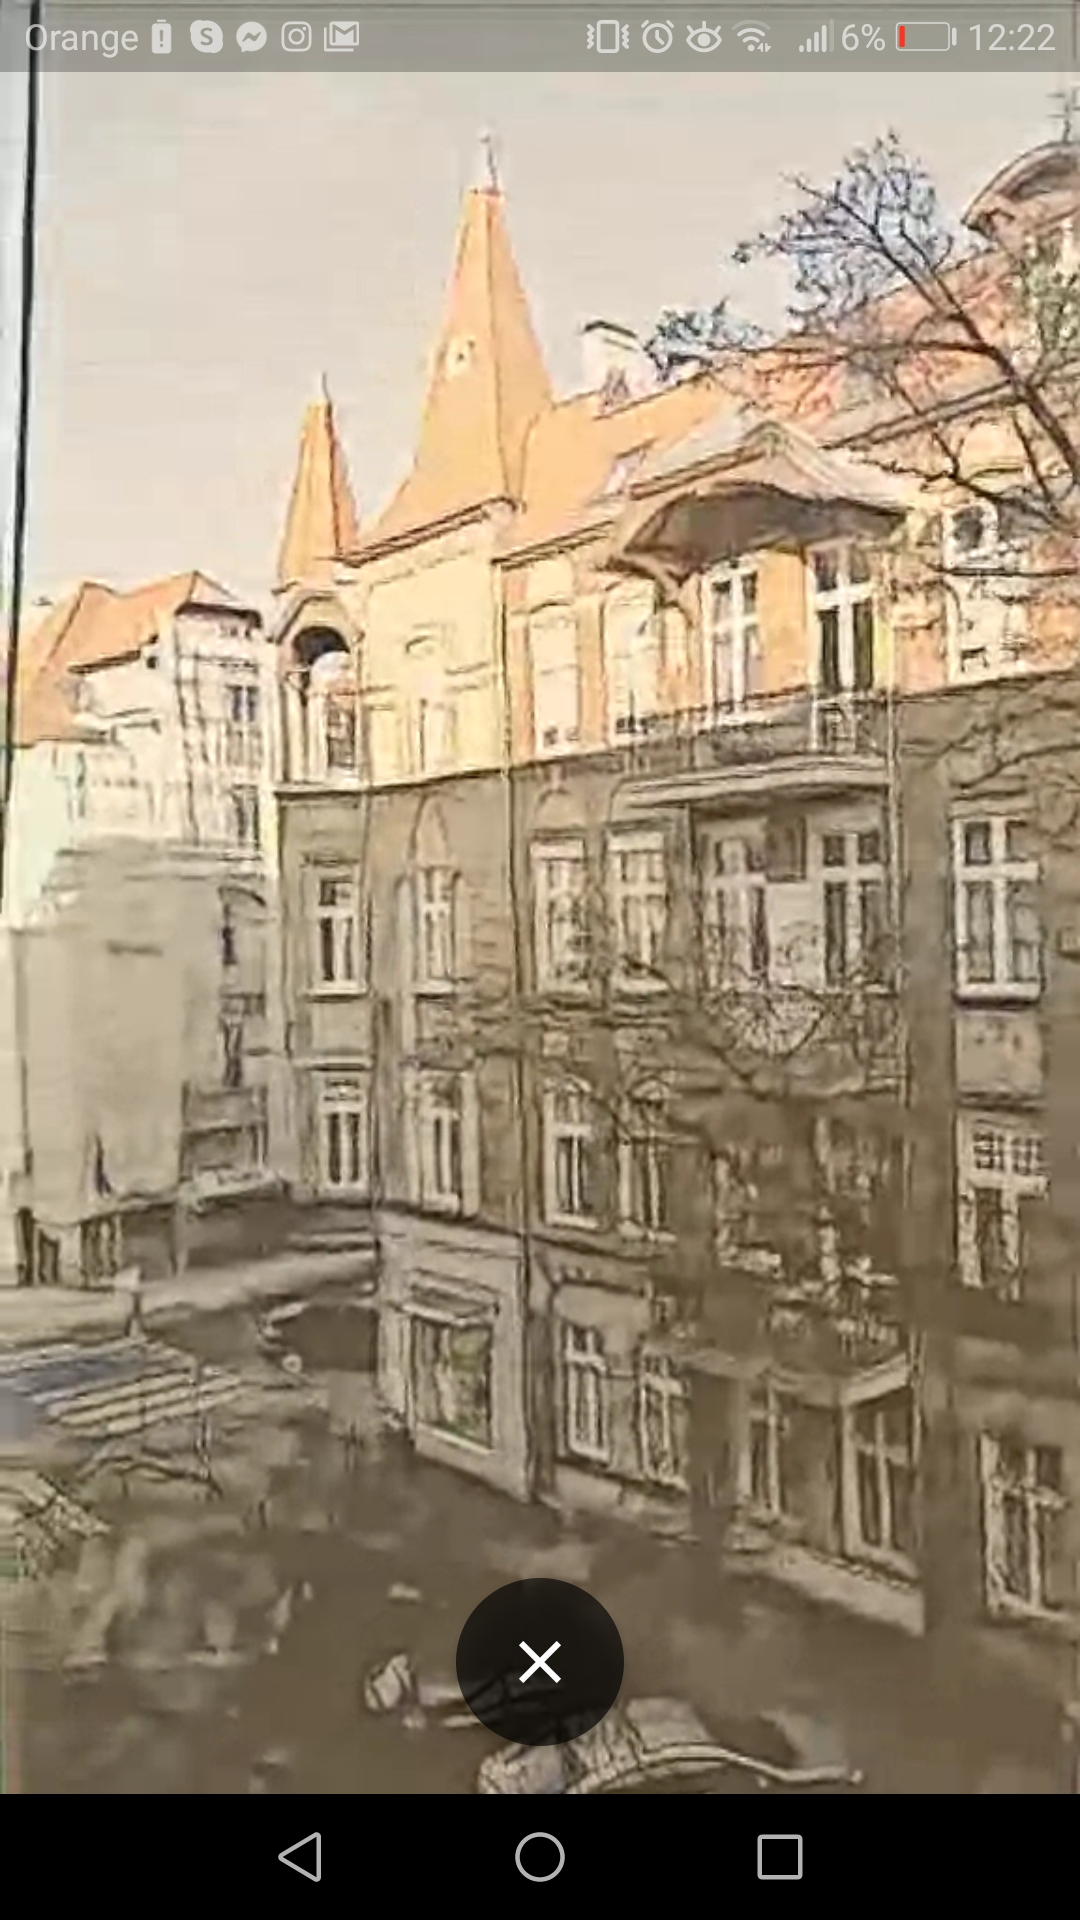
\includegraphics[width = 0.13\linewidth]{Images/app_photos/kamienica/salon.jpg} &
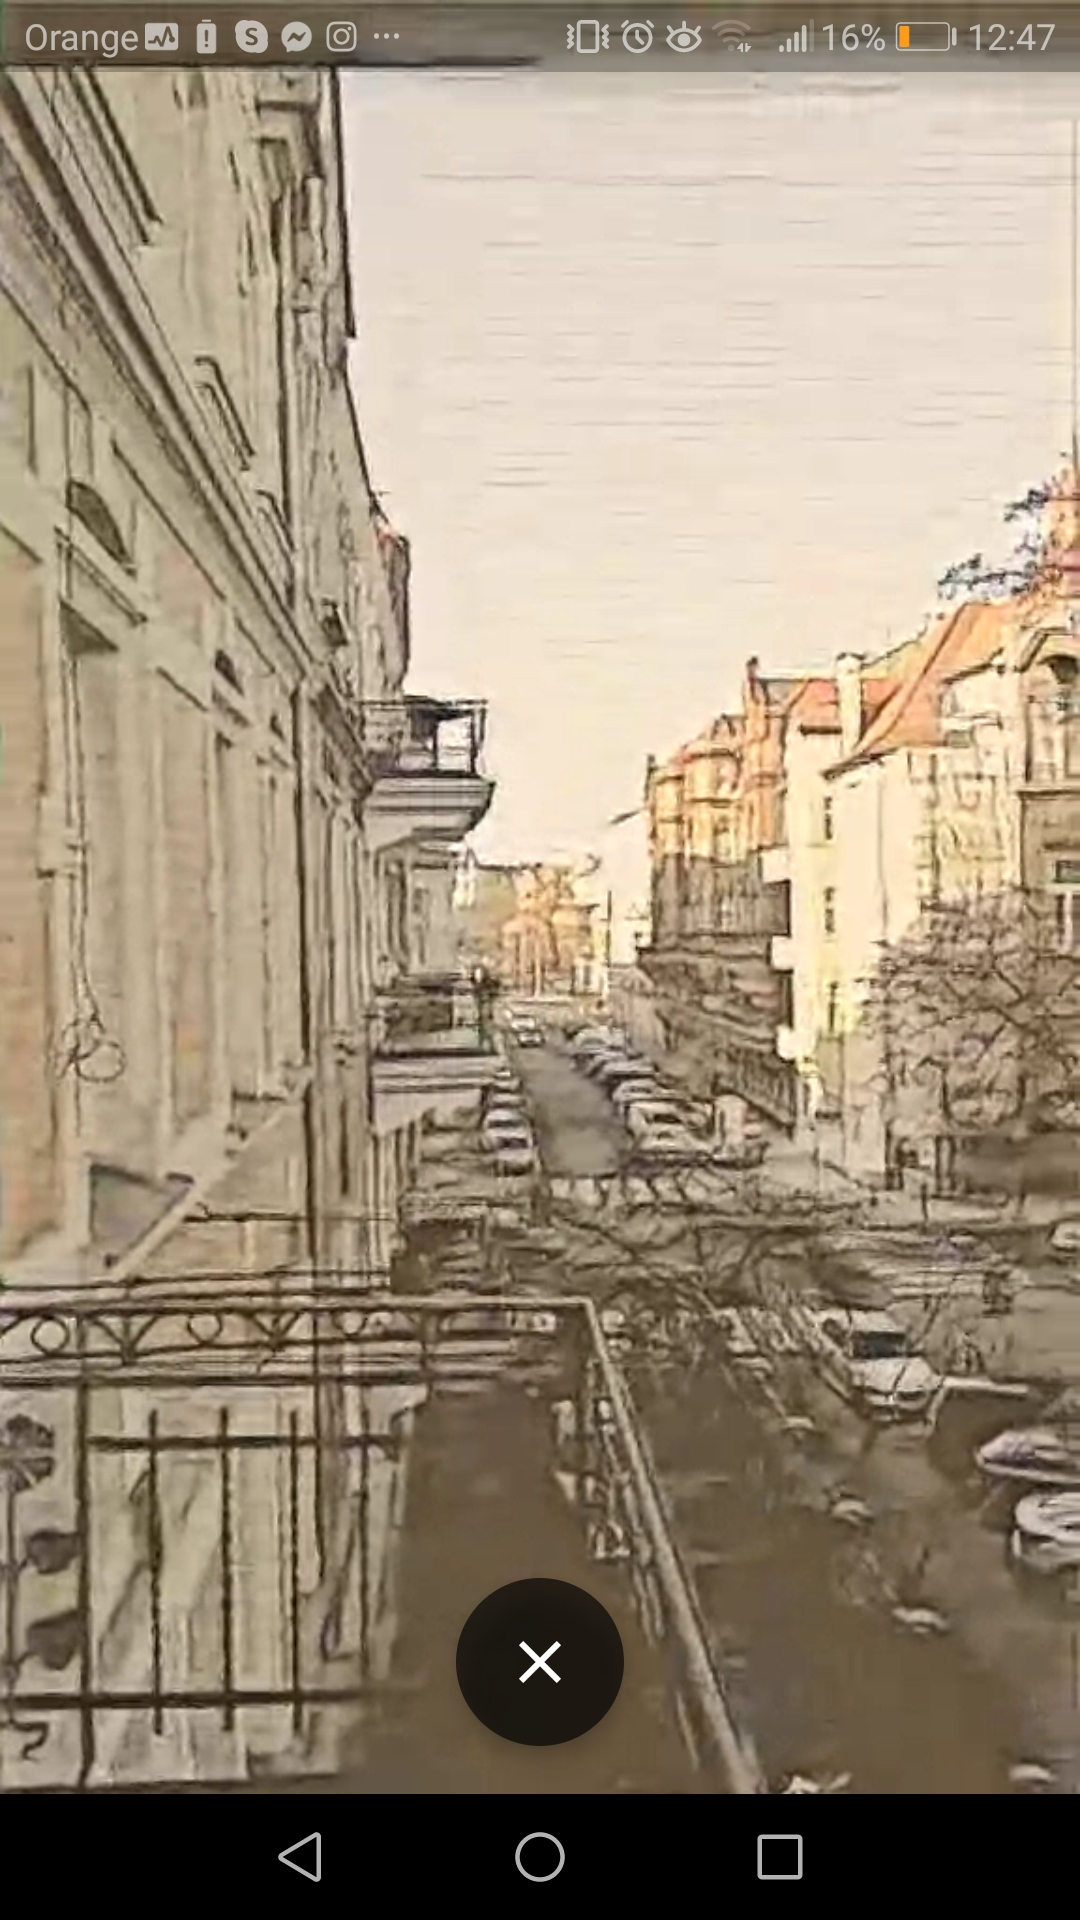
\includegraphics[width = 0.13\linewidth]{Images/app_photos/ulica/salon.jpg} \\

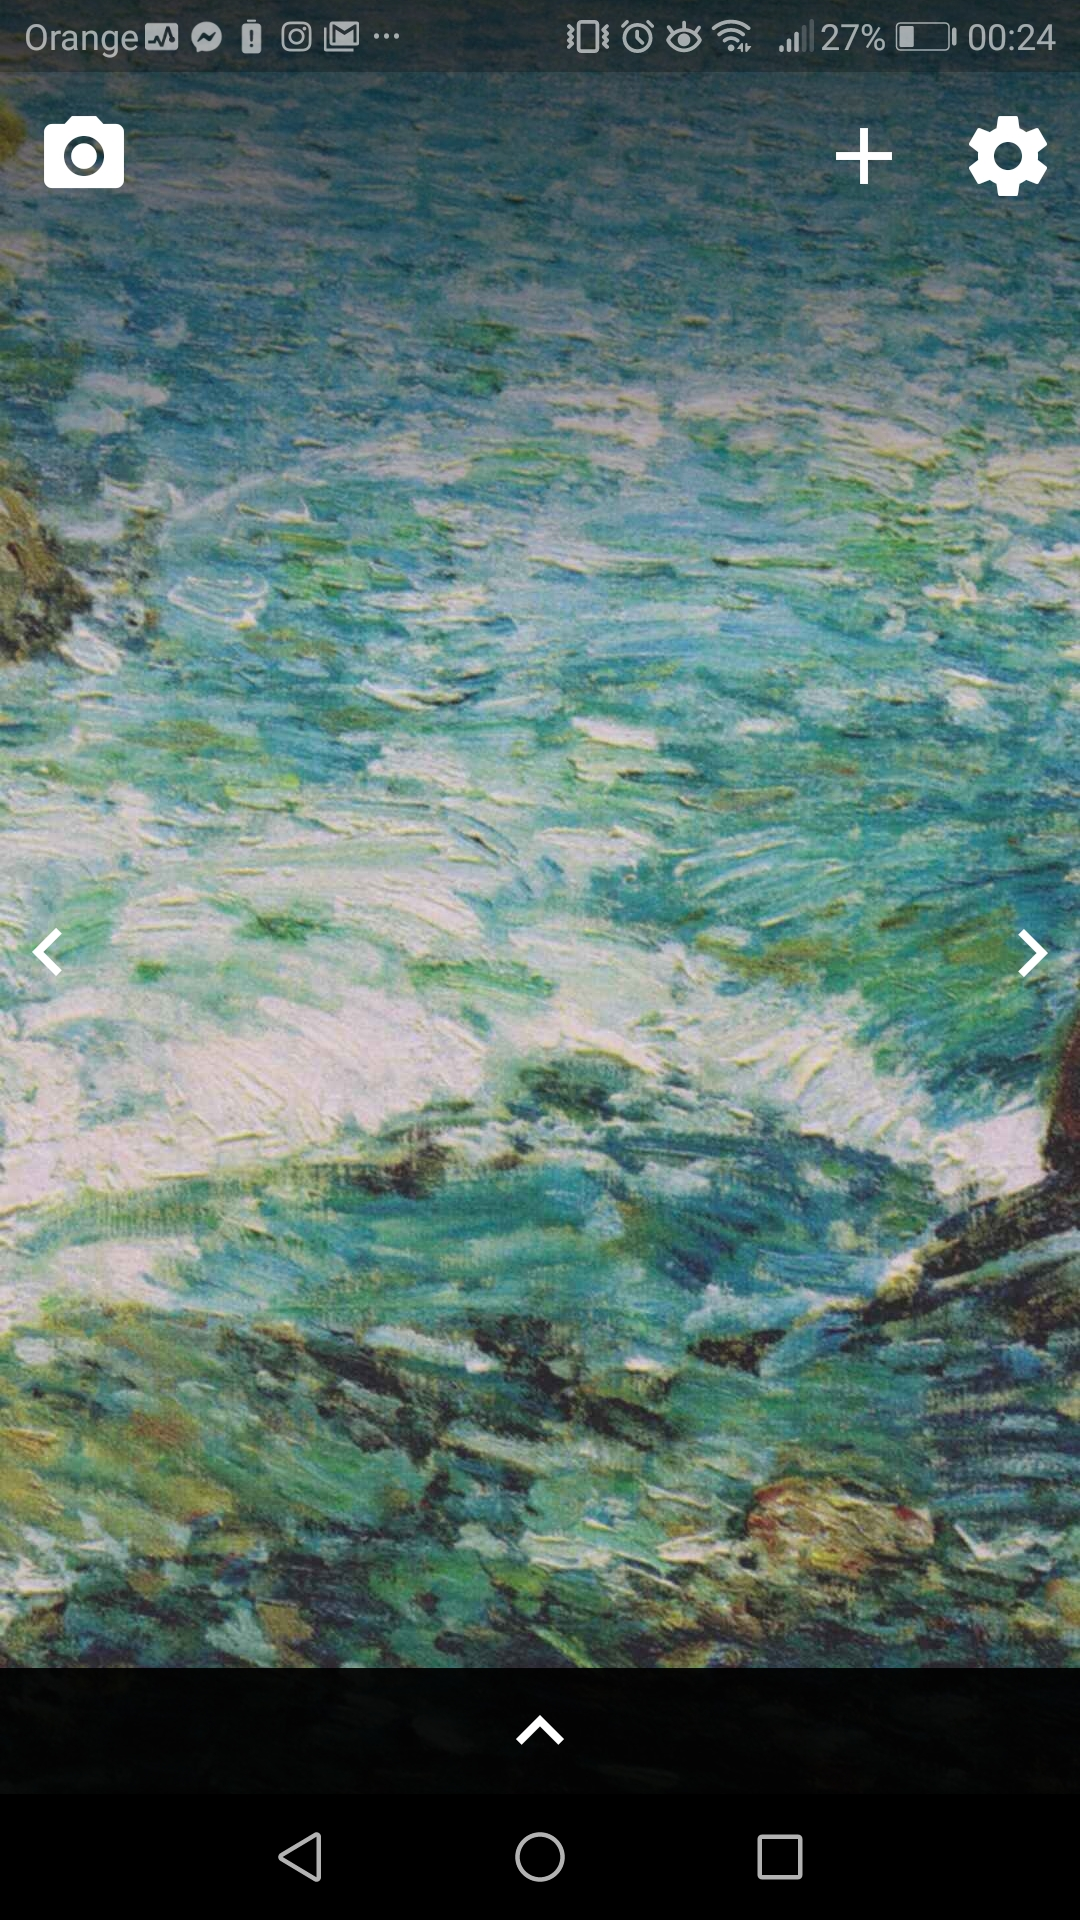
\includegraphics[width = 0.13\linewidth]{Images/app_photos/filters/ocean.jpg} &
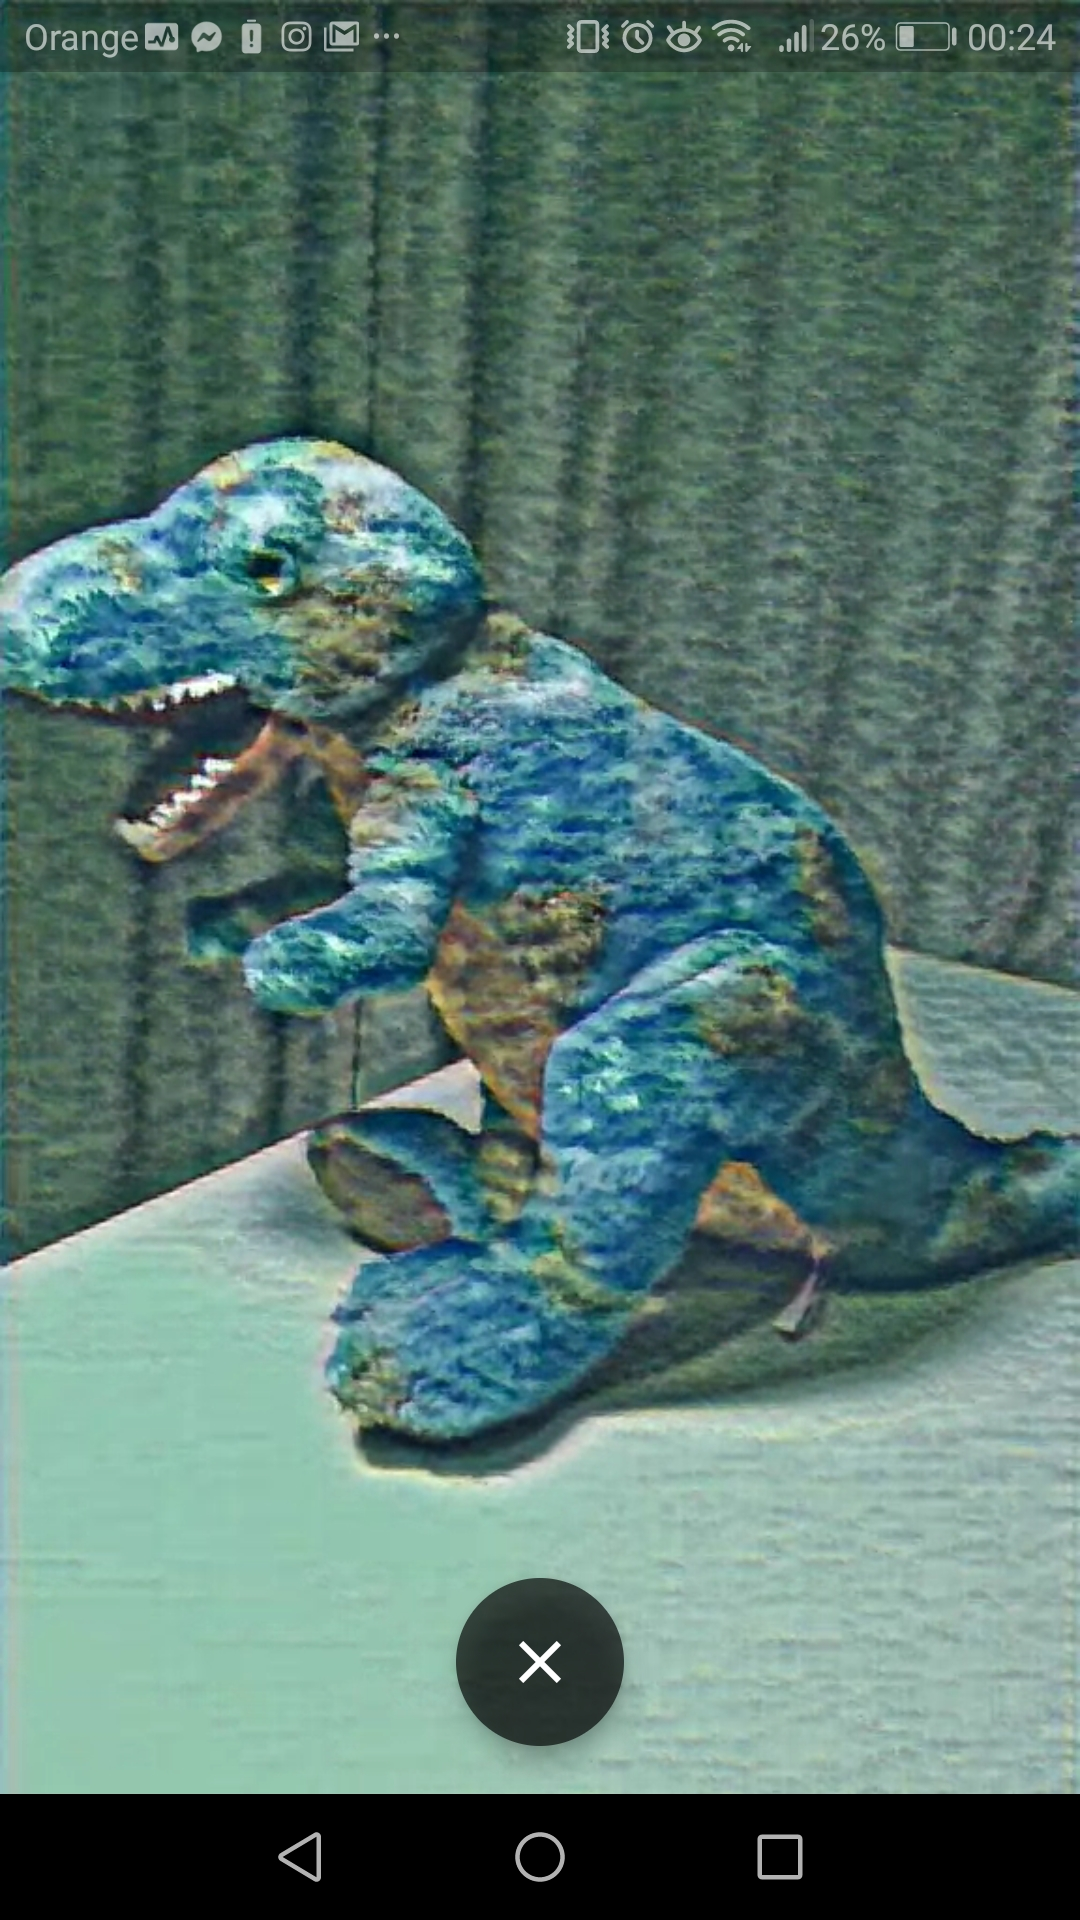
\includegraphics[width = 0.13\linewidth]{Images/app_photos/dino/ocean.jpg} &
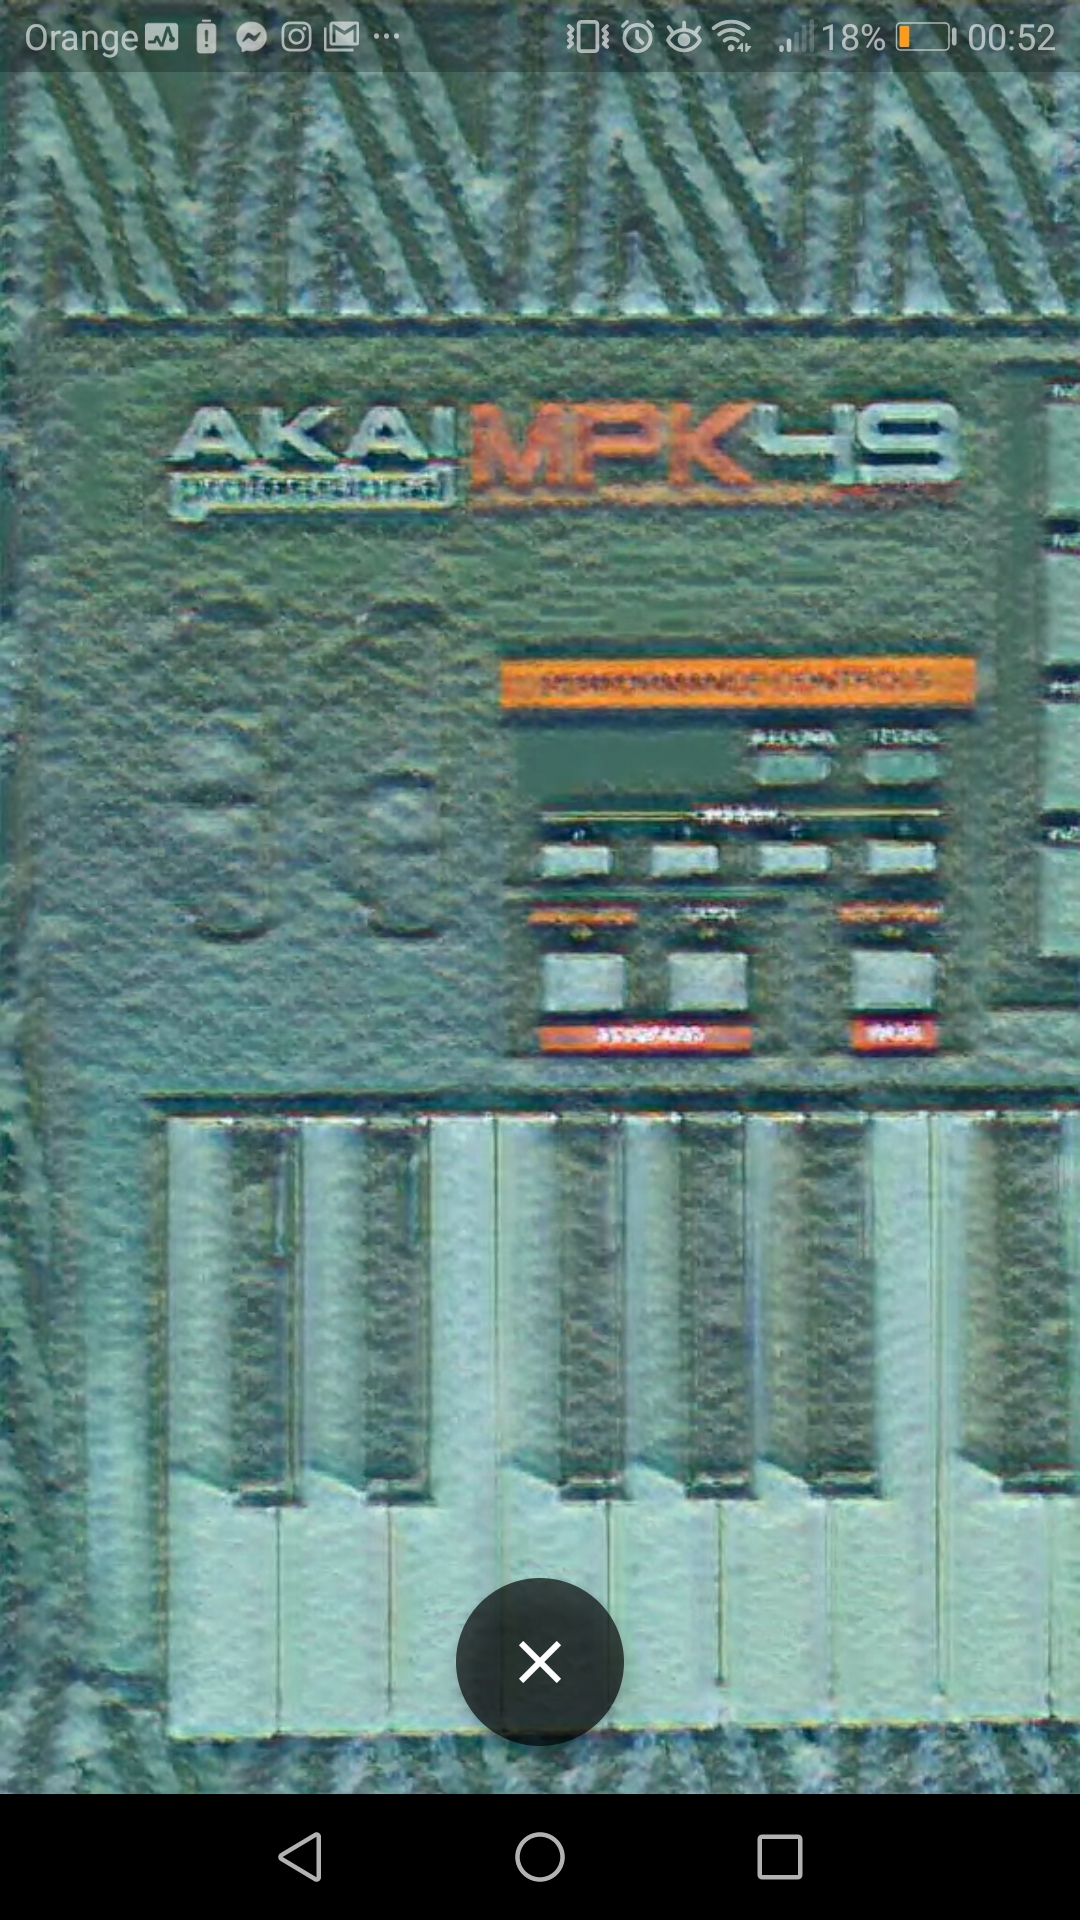
\includegraphics[width = 0.13\linewidth]{Images/app_photos/akai/ocean.jpg} &
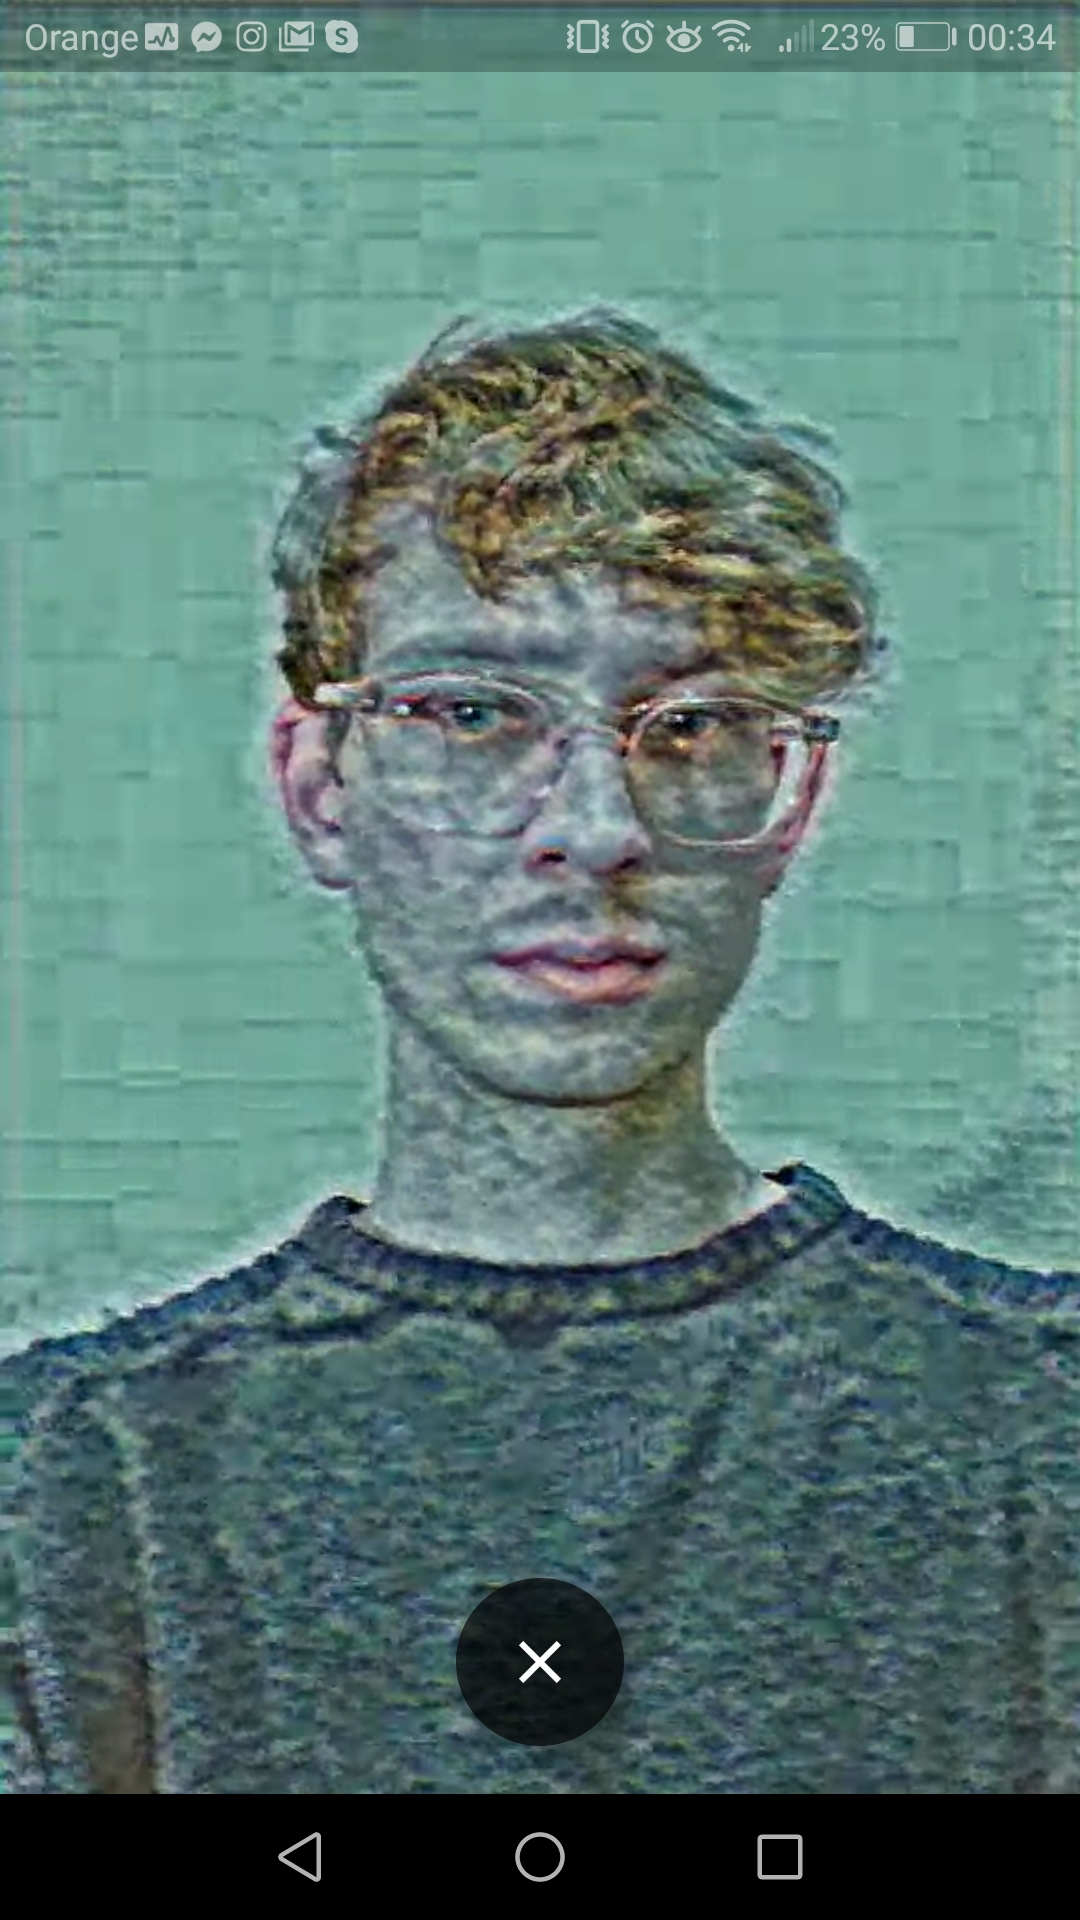
\includegraphics[width = 0.13\linewidth]{Images/app_photos/me/ocean.jpg} &
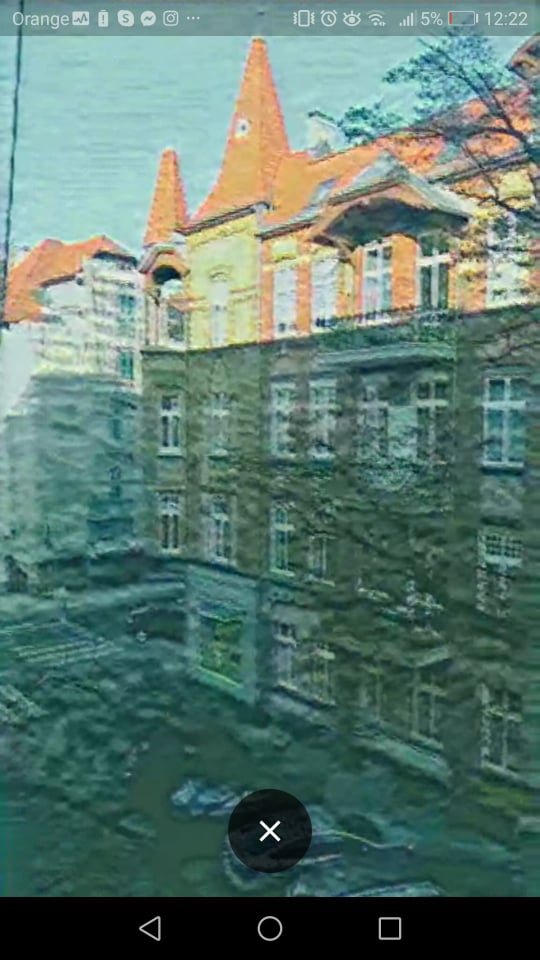
\includegraphics[width = 0.13\linewidth]{Images/app_photos/kamienica/ocean.jpg} &
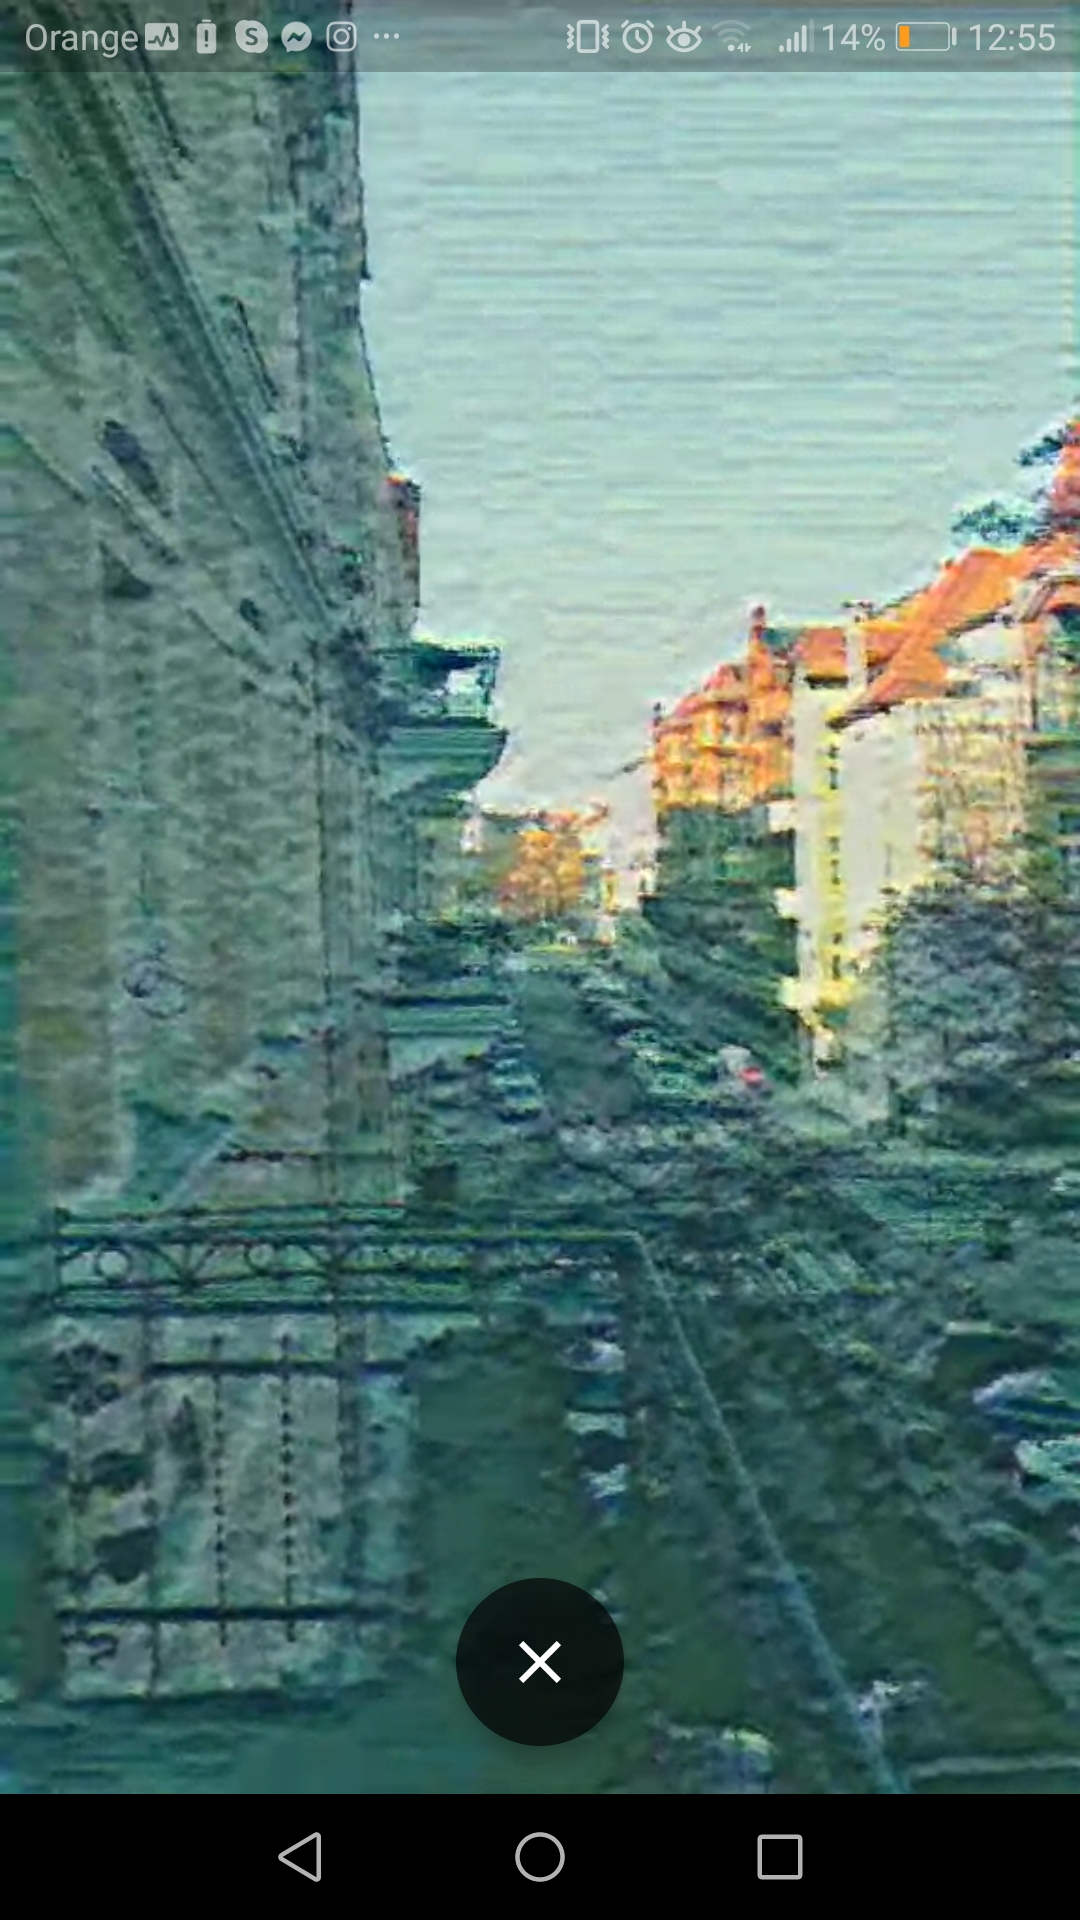
\includegraphics[width = 0.13\linewidth]{Images/app_photos/ulica/ocean.jpg} \\

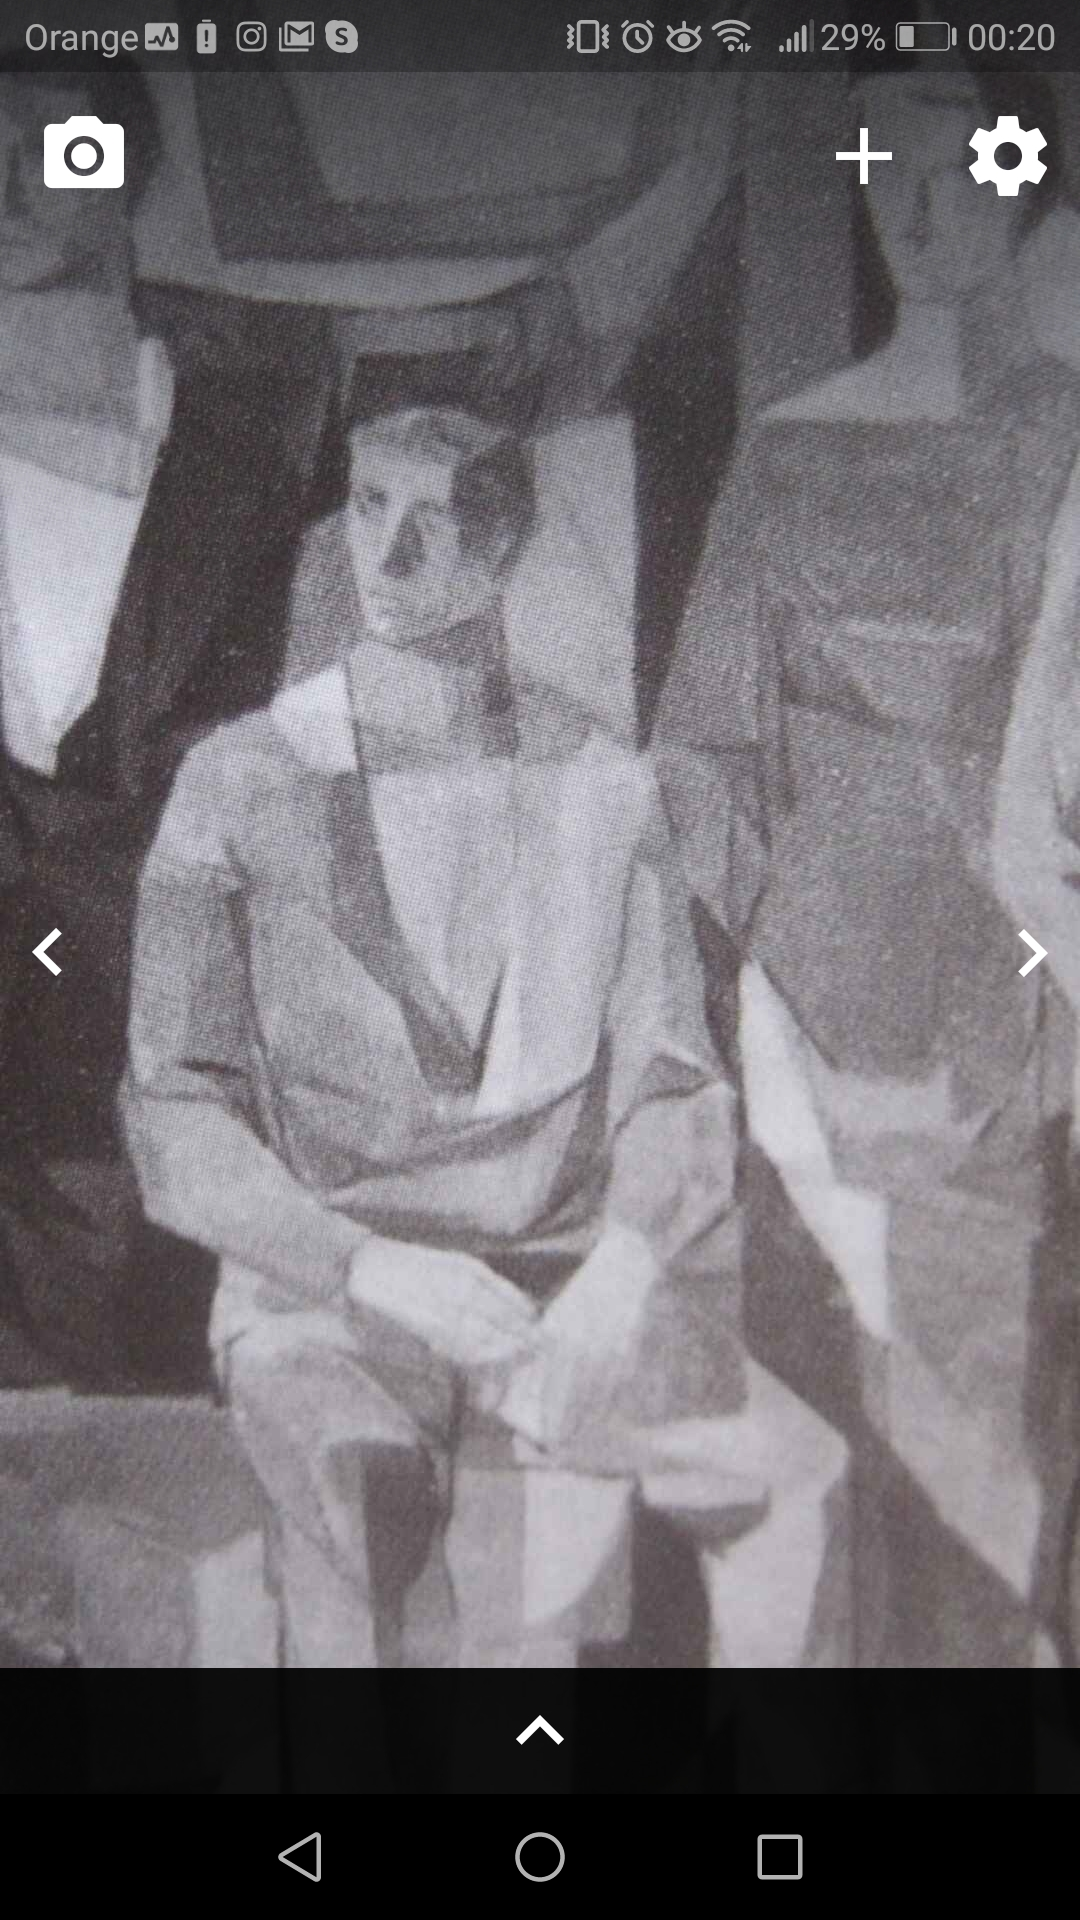
\includegraphics[width = 0.13\linewidth]{Images/app_photos/filters/draw.jpg} &
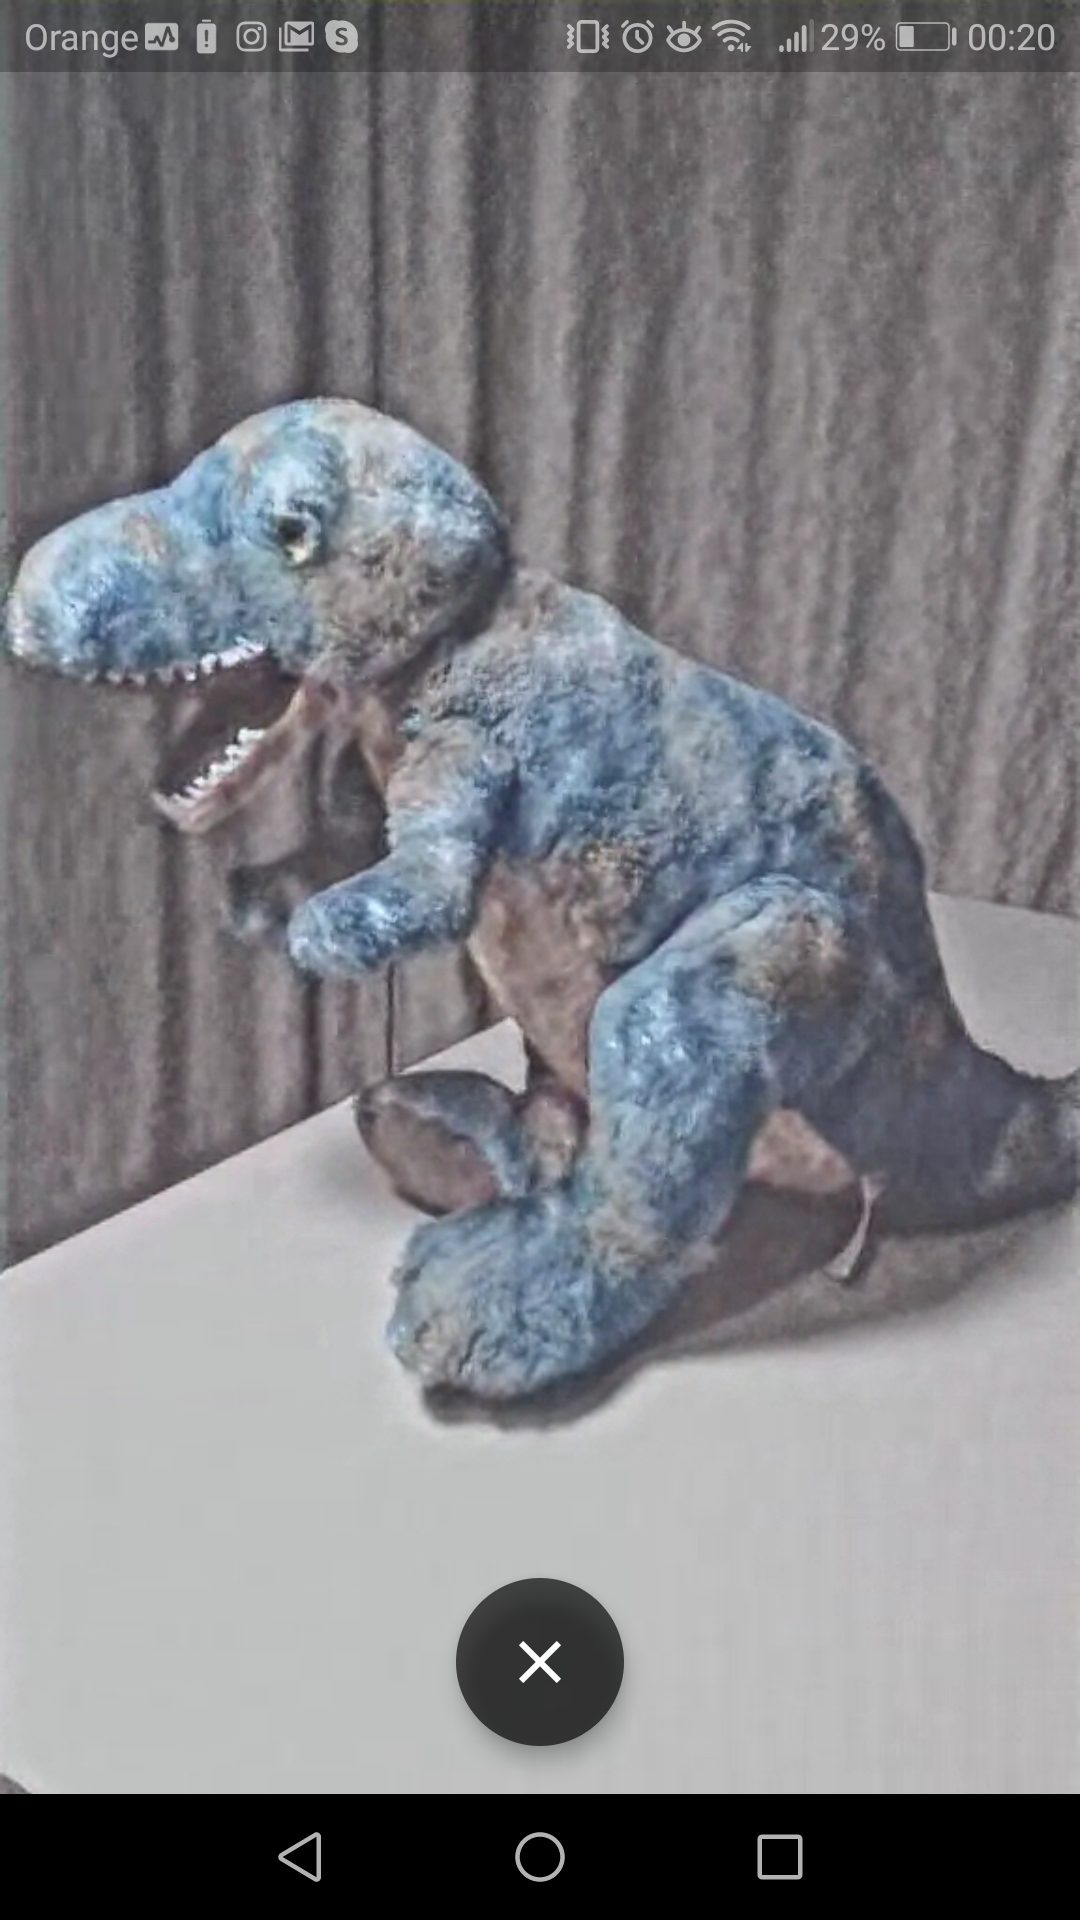
\includegraphics[width = 0.13\linewidth]{Images/app_photos/dino/draw.jpg} &
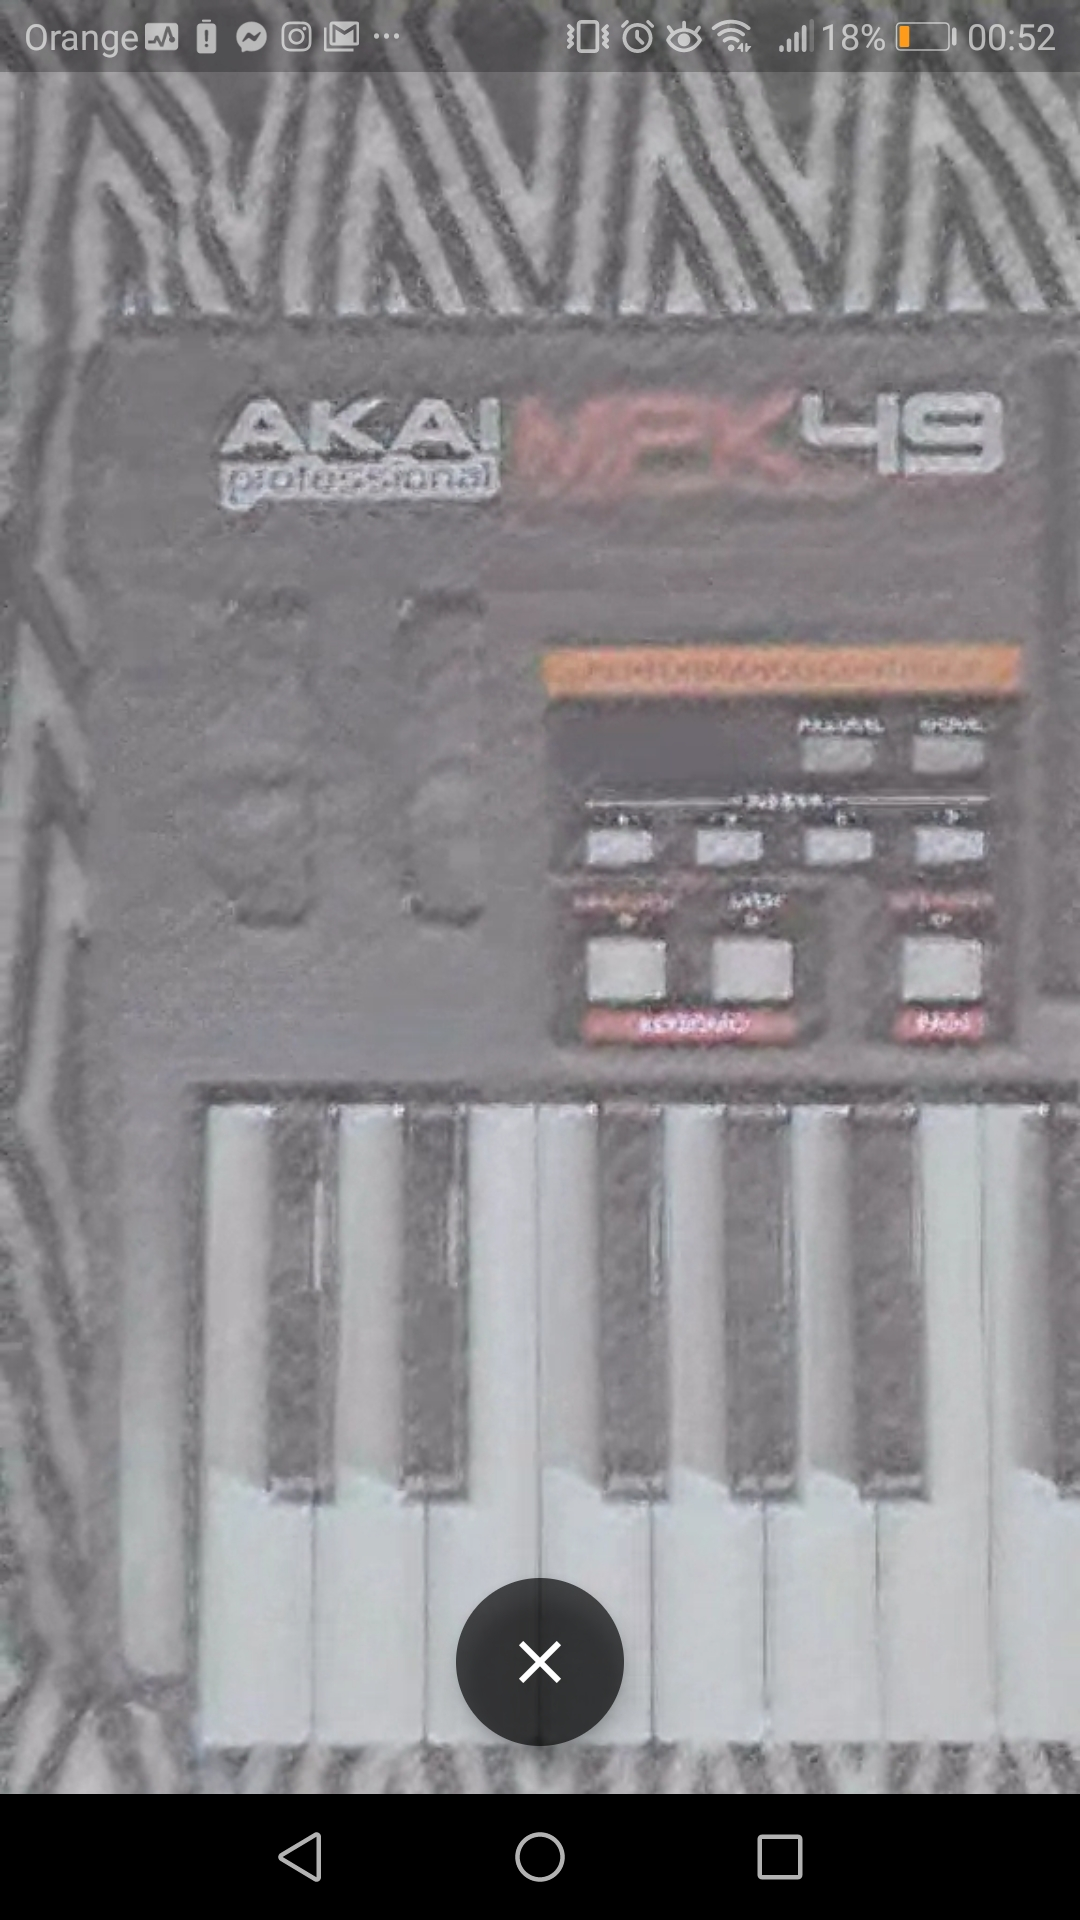
\includegraphics[width = 0.13\linewidth]{Images/app_photos/akai/draw.jpg} &
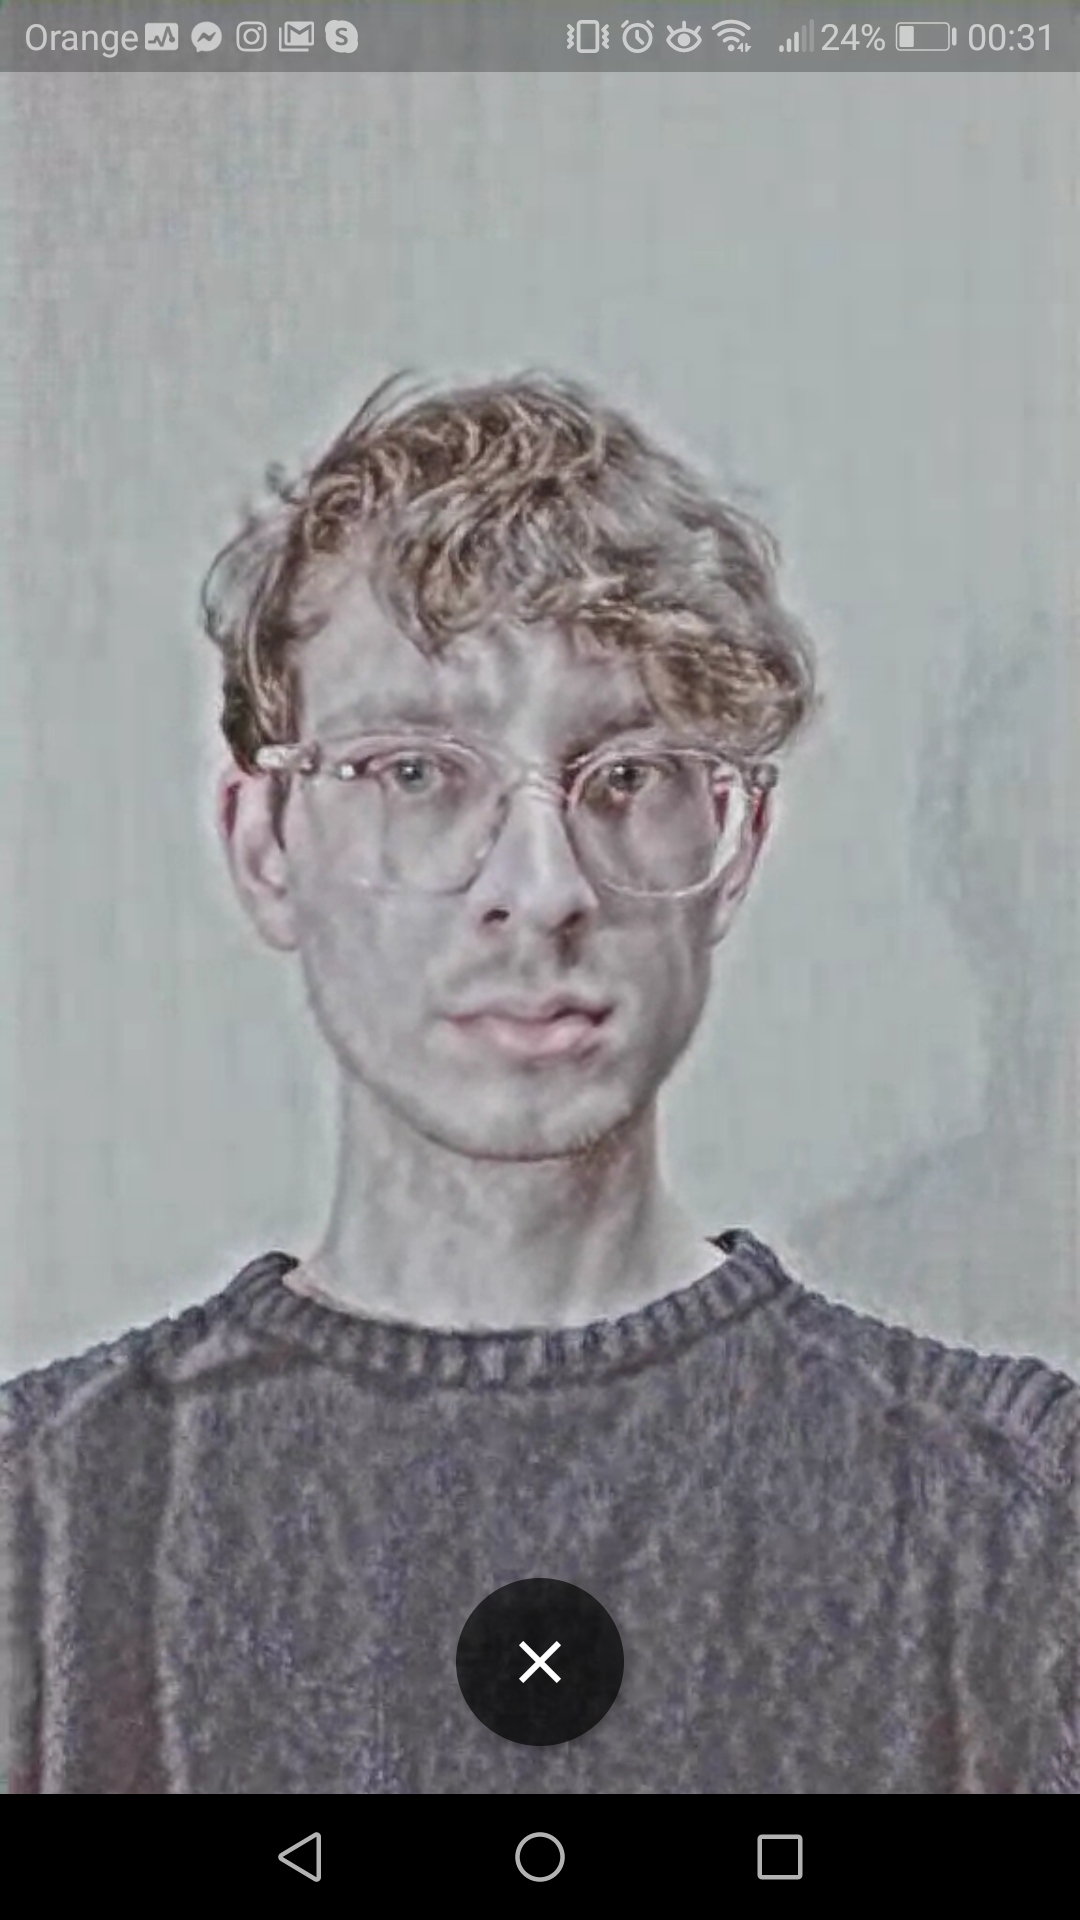
\includegraphics[width = 0.13\linewidth]{Images/app_photos/me/draw.jpg} &
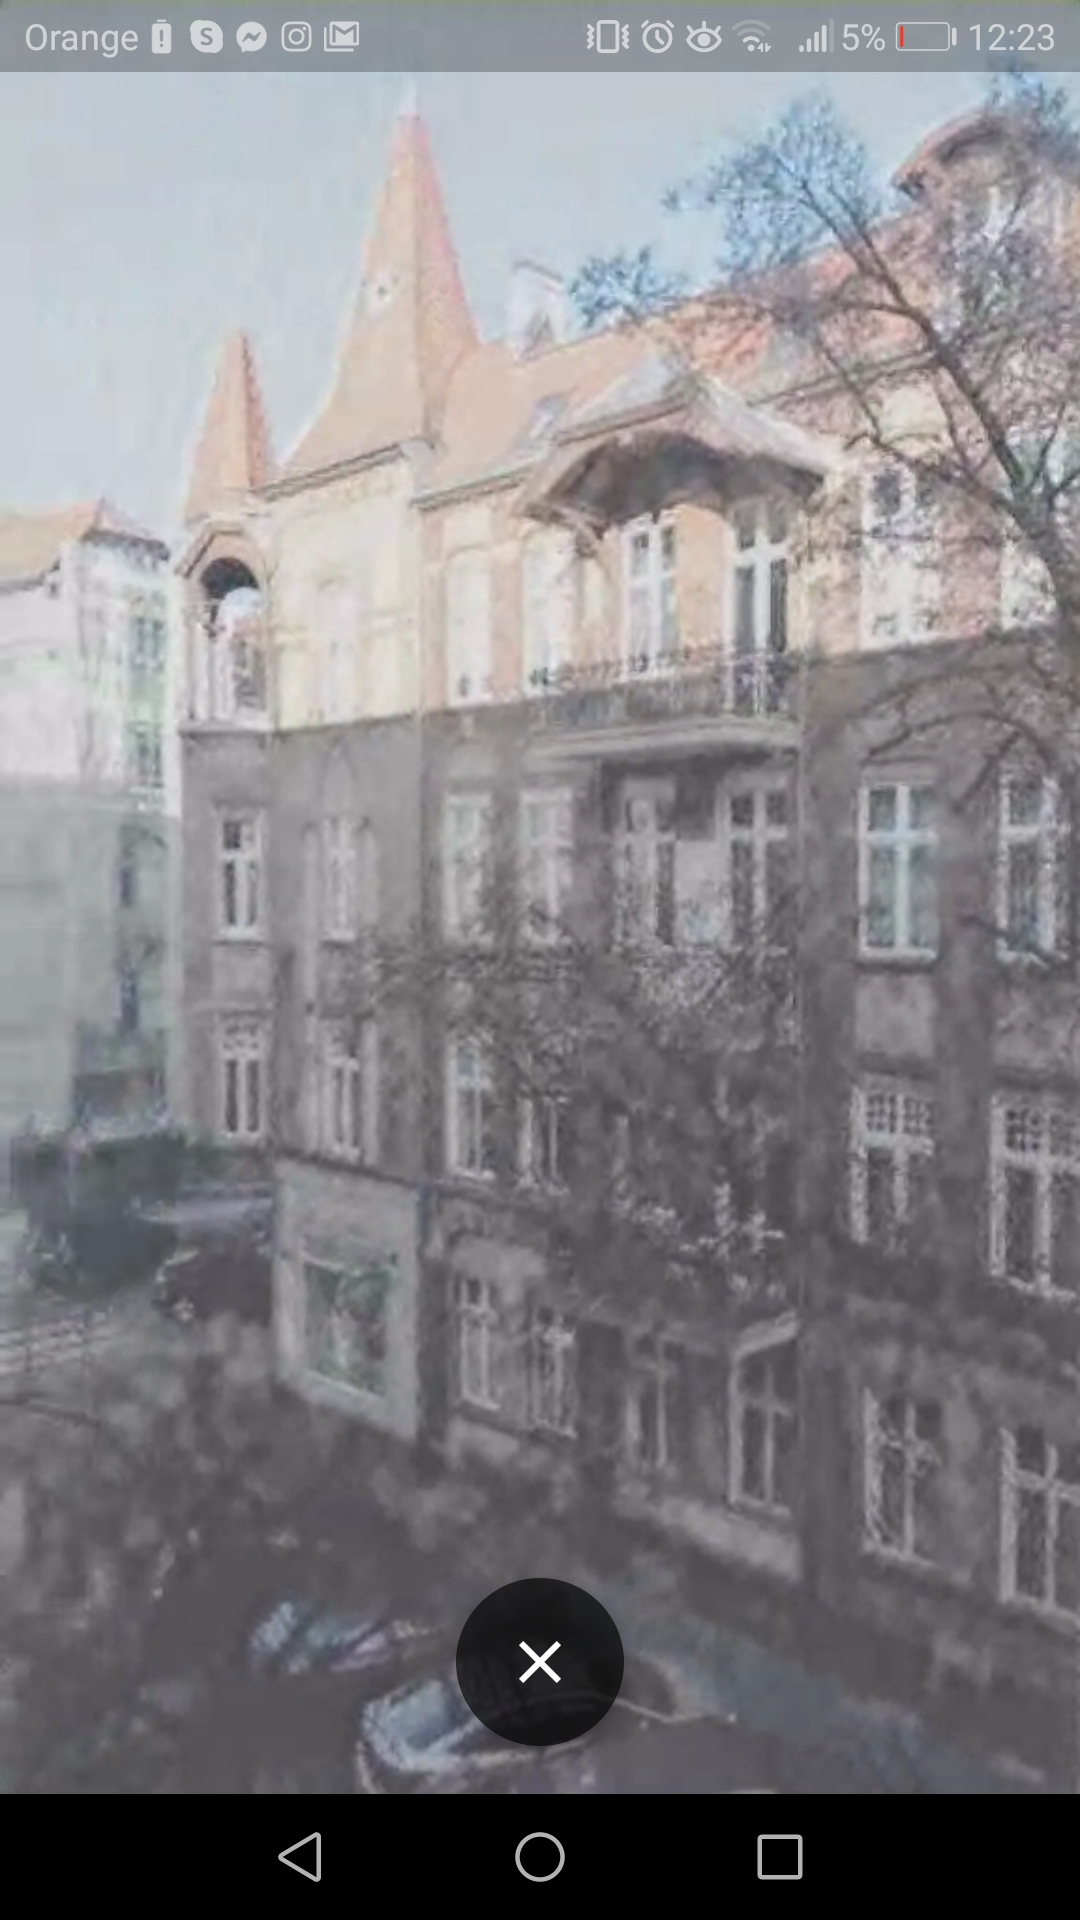
\includegraphics[width = 0.13\linewidth]{Images/app_photos/kamienica/draw.jpg} &
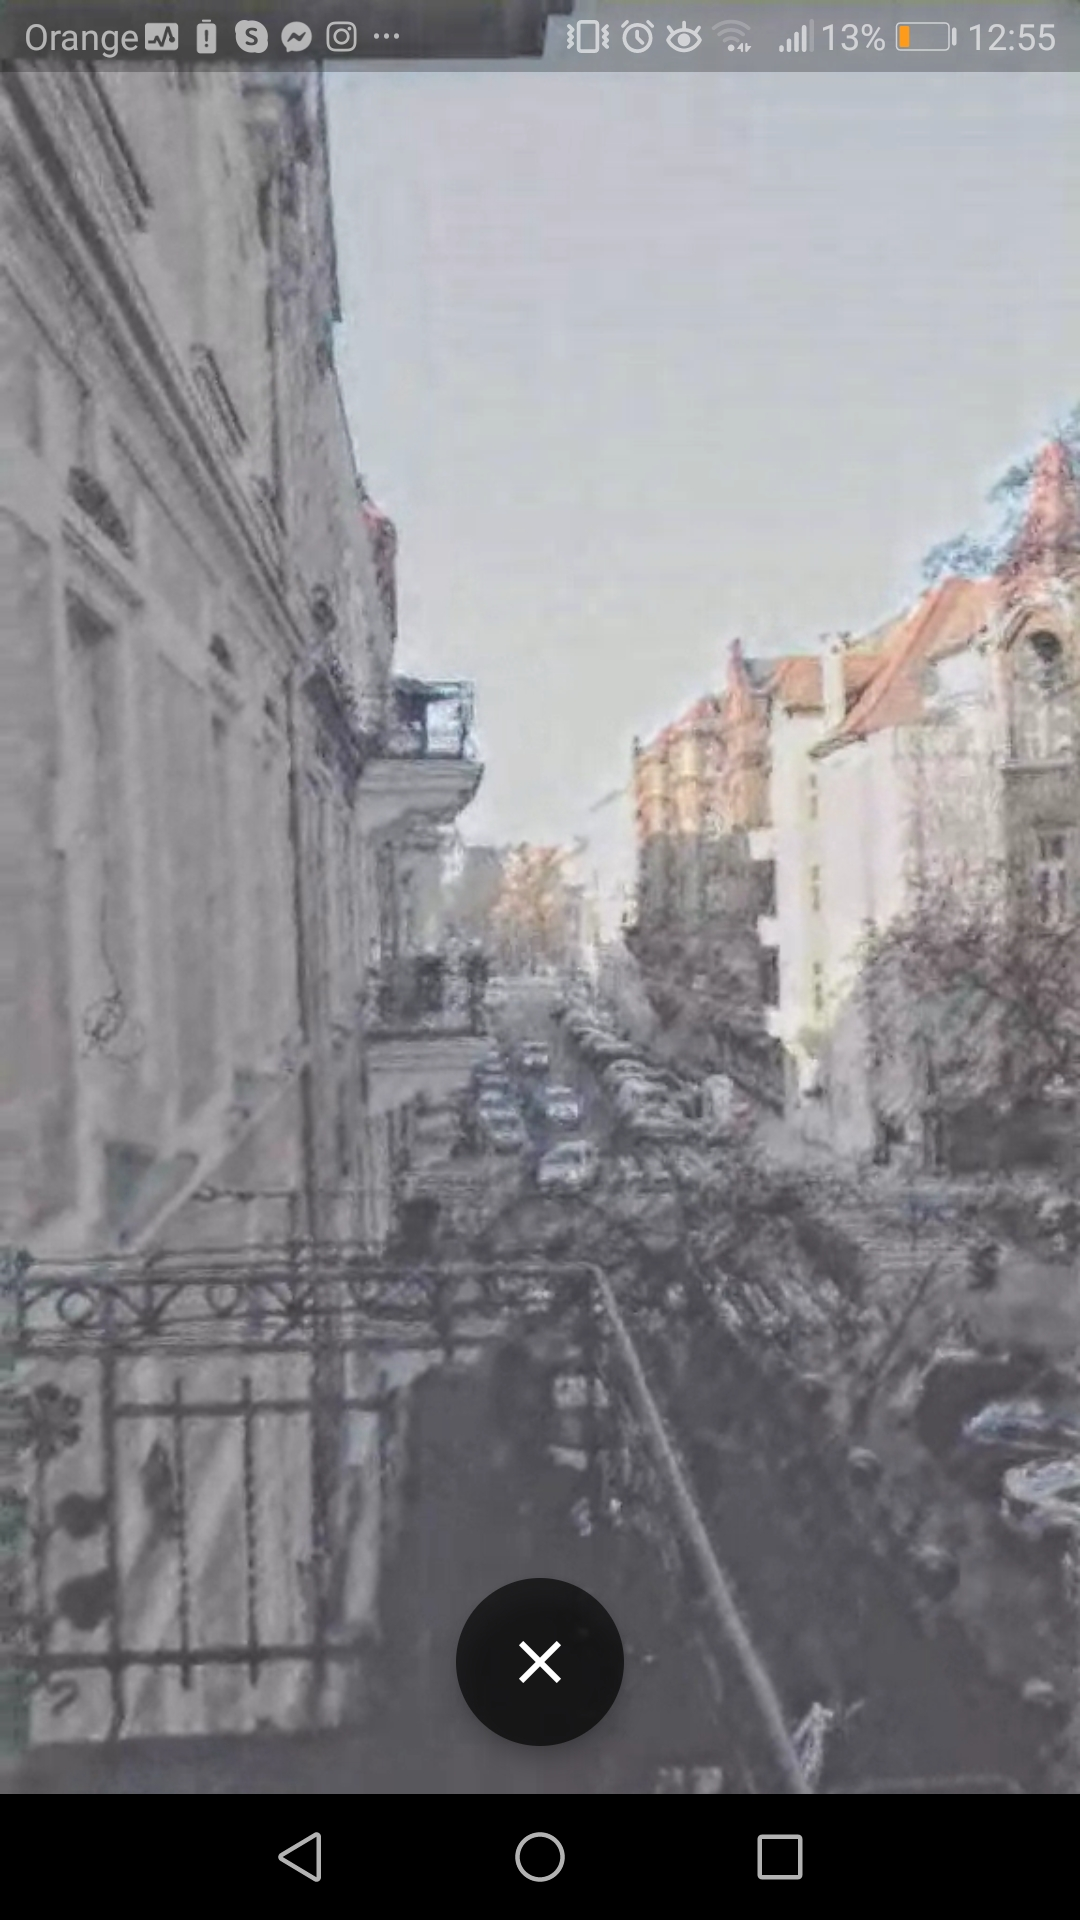
\includegraphics[width = 0.13\linewidth]{Images/app_photos/ulica/draw.jpg} \\

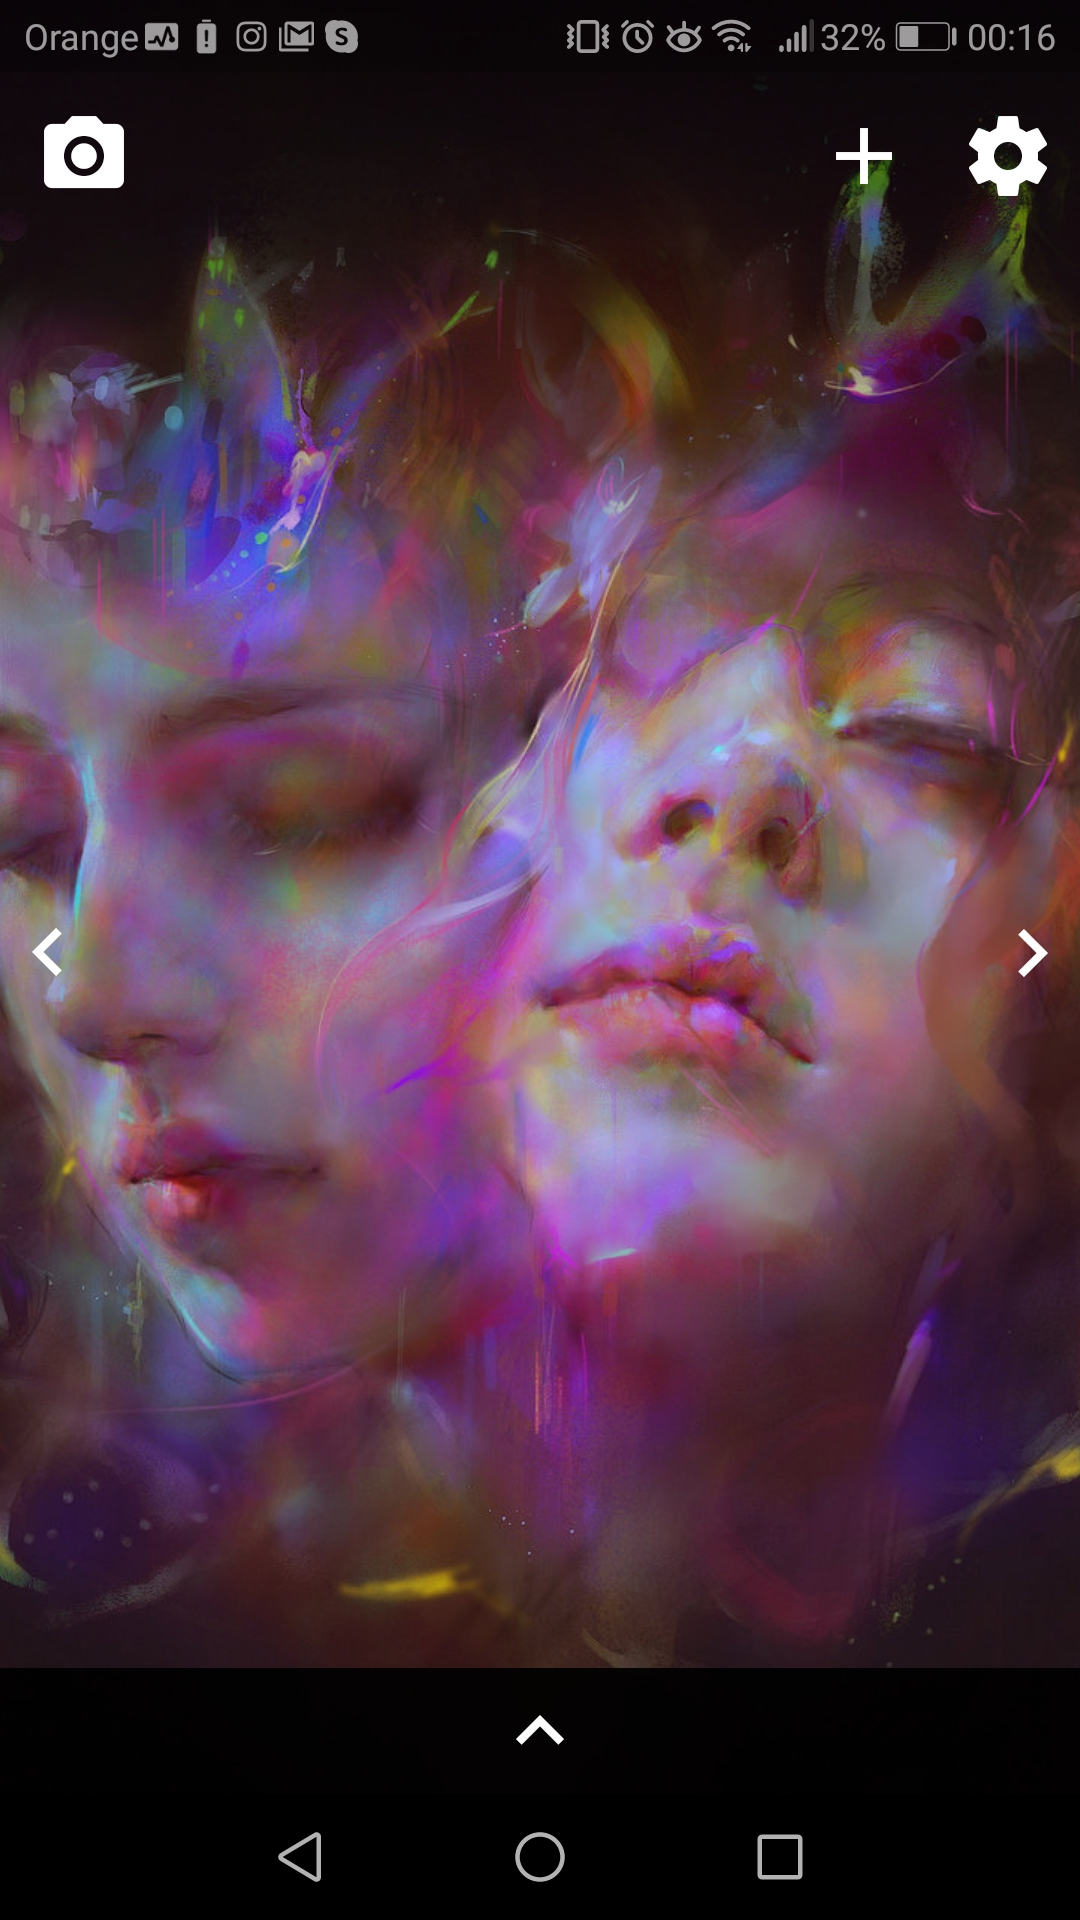
\includegraphics[width = 0.13\linewidth]{Images/app_photos/filters/lets.jpg} &
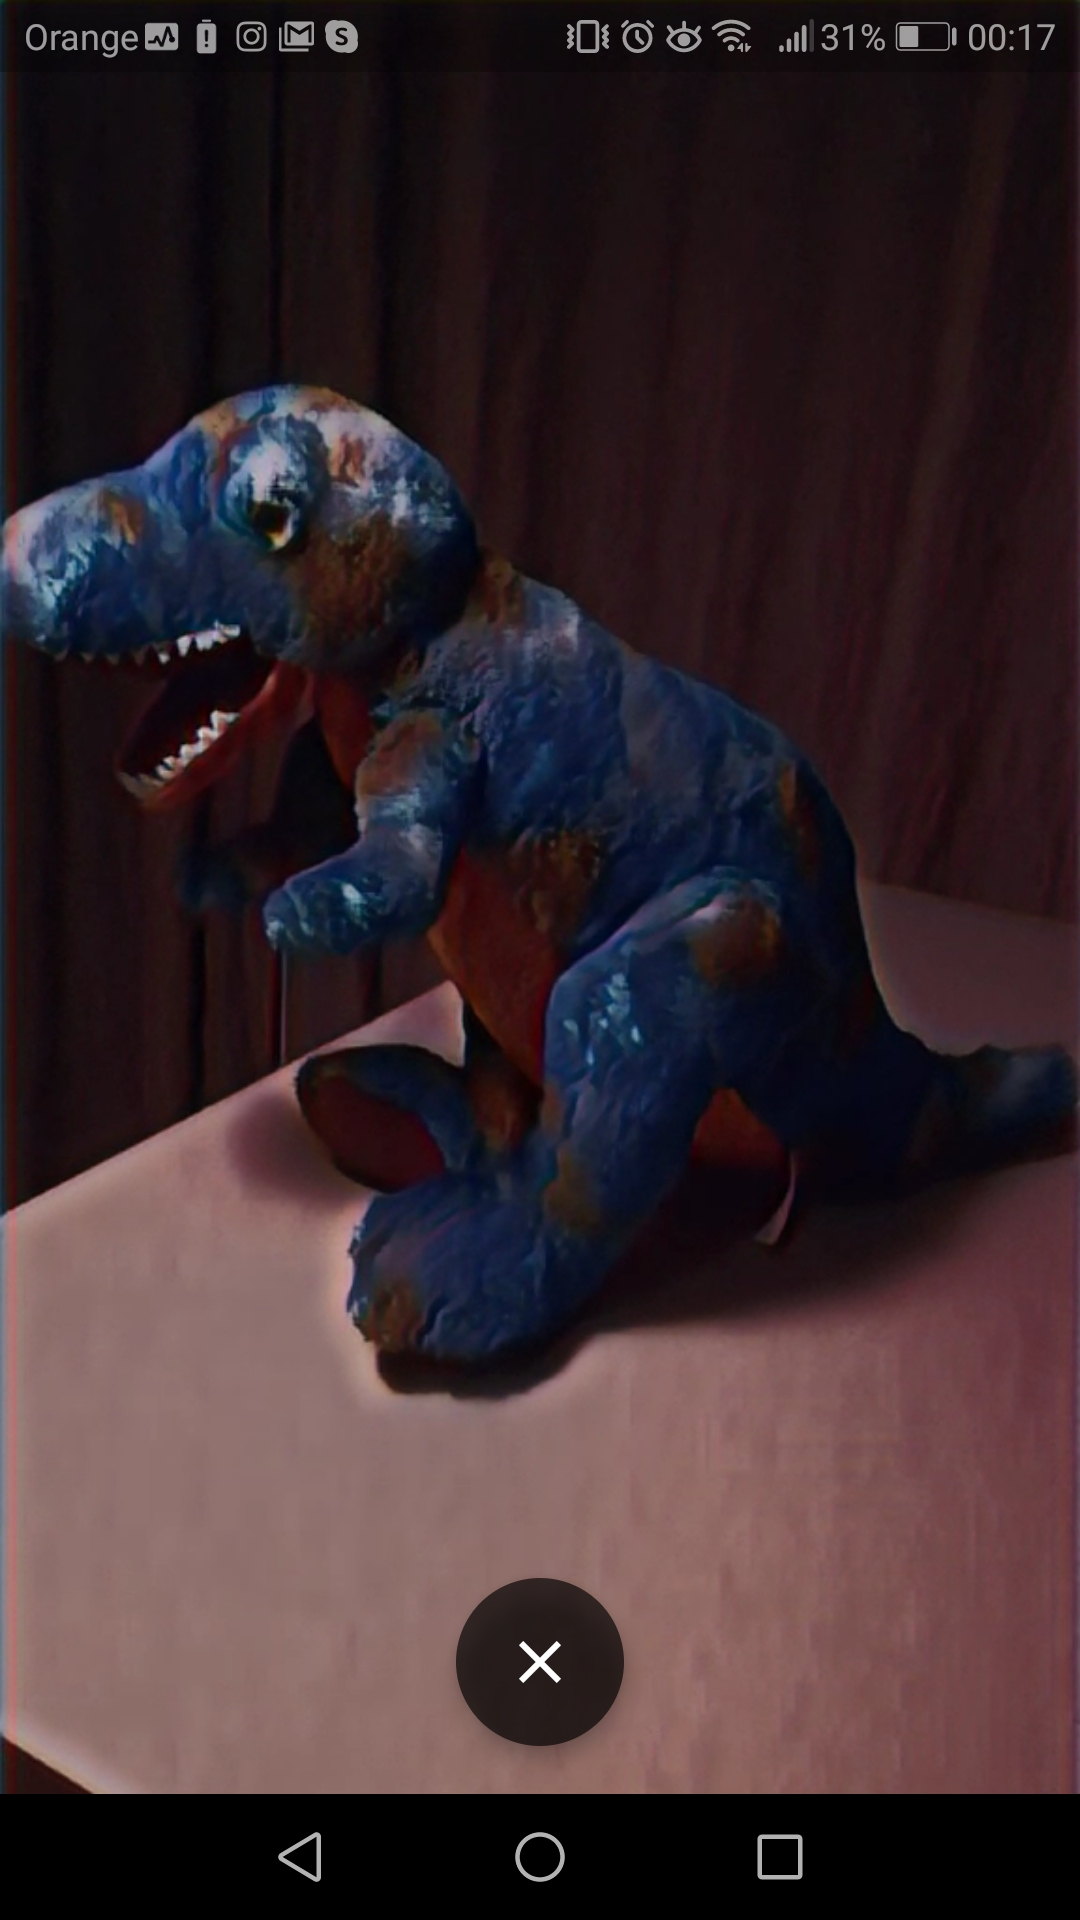
\includegraphics[width = 0.13\linewidth]{Images/app_photos/dino/lets.jpg} &
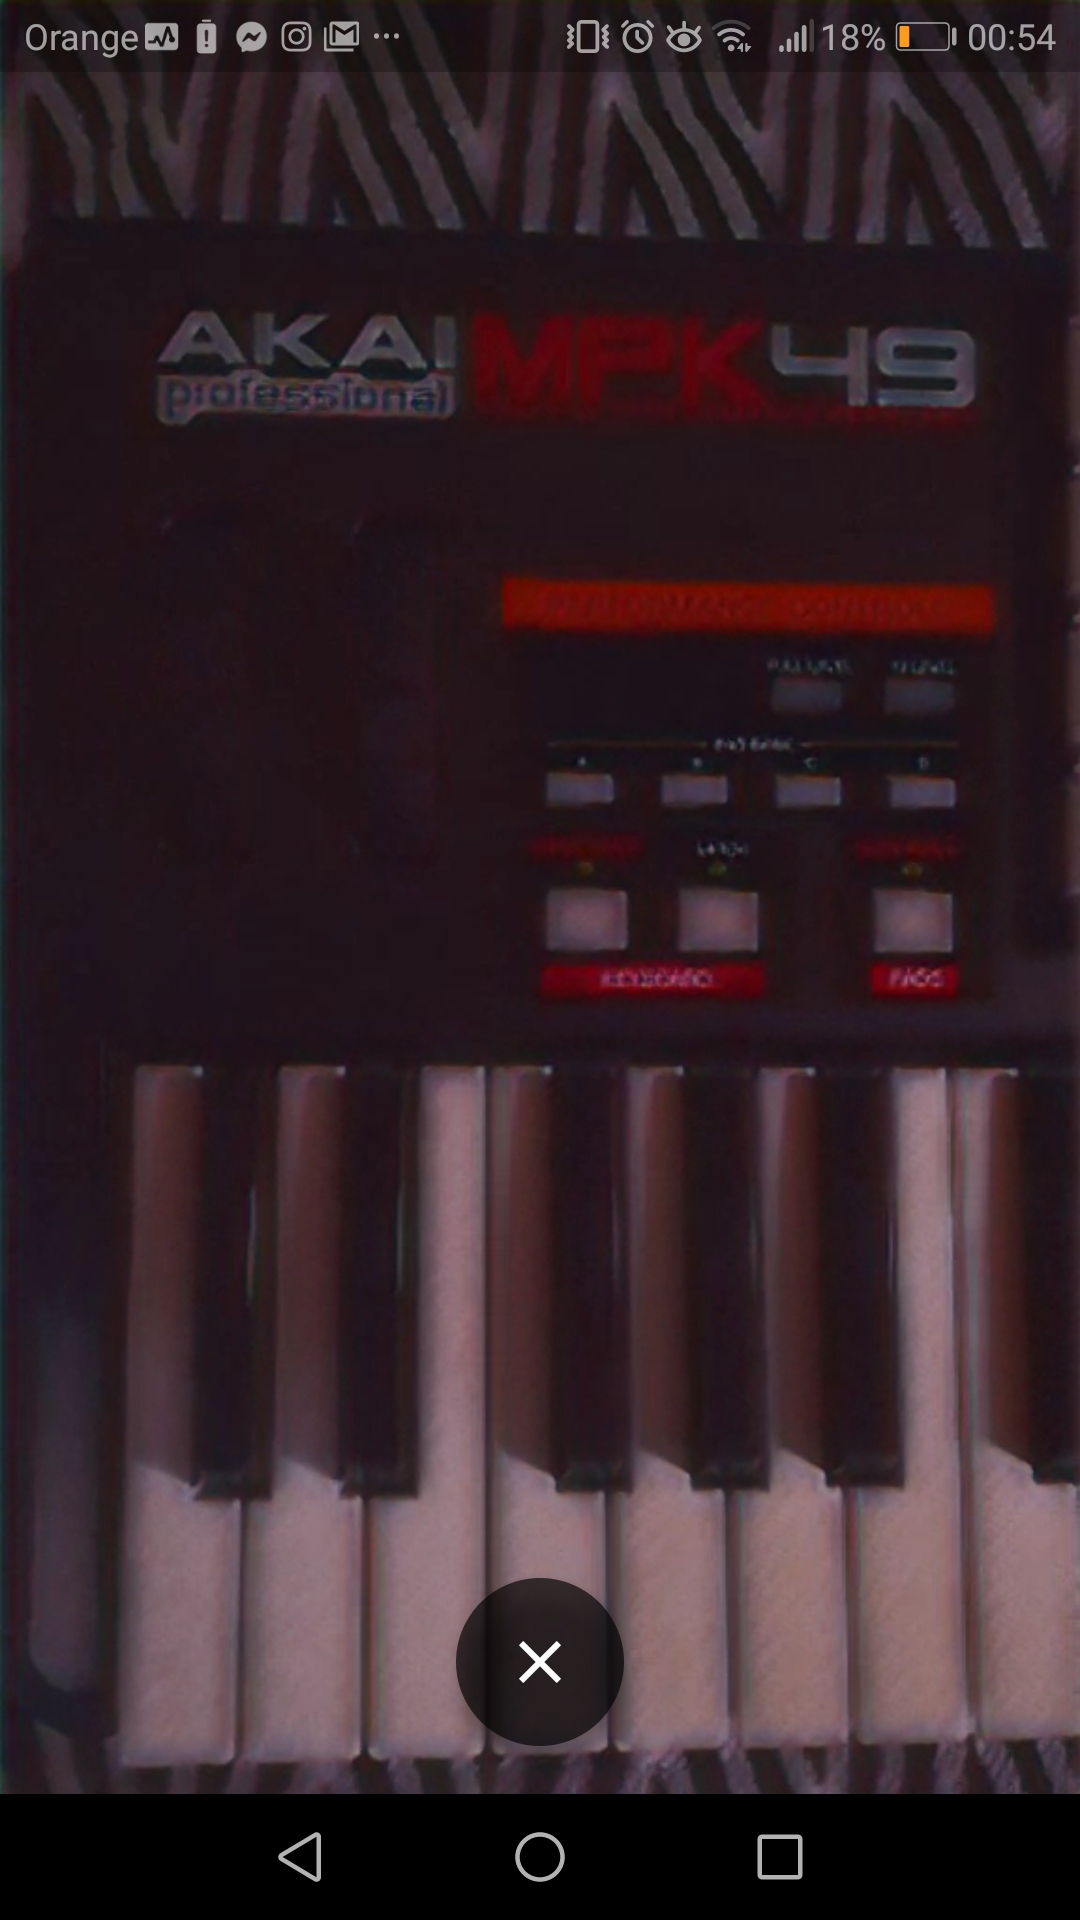
\includegraphics[width = 0.13\linewidth]{Images/app_photos/akai/lets.jpg} &
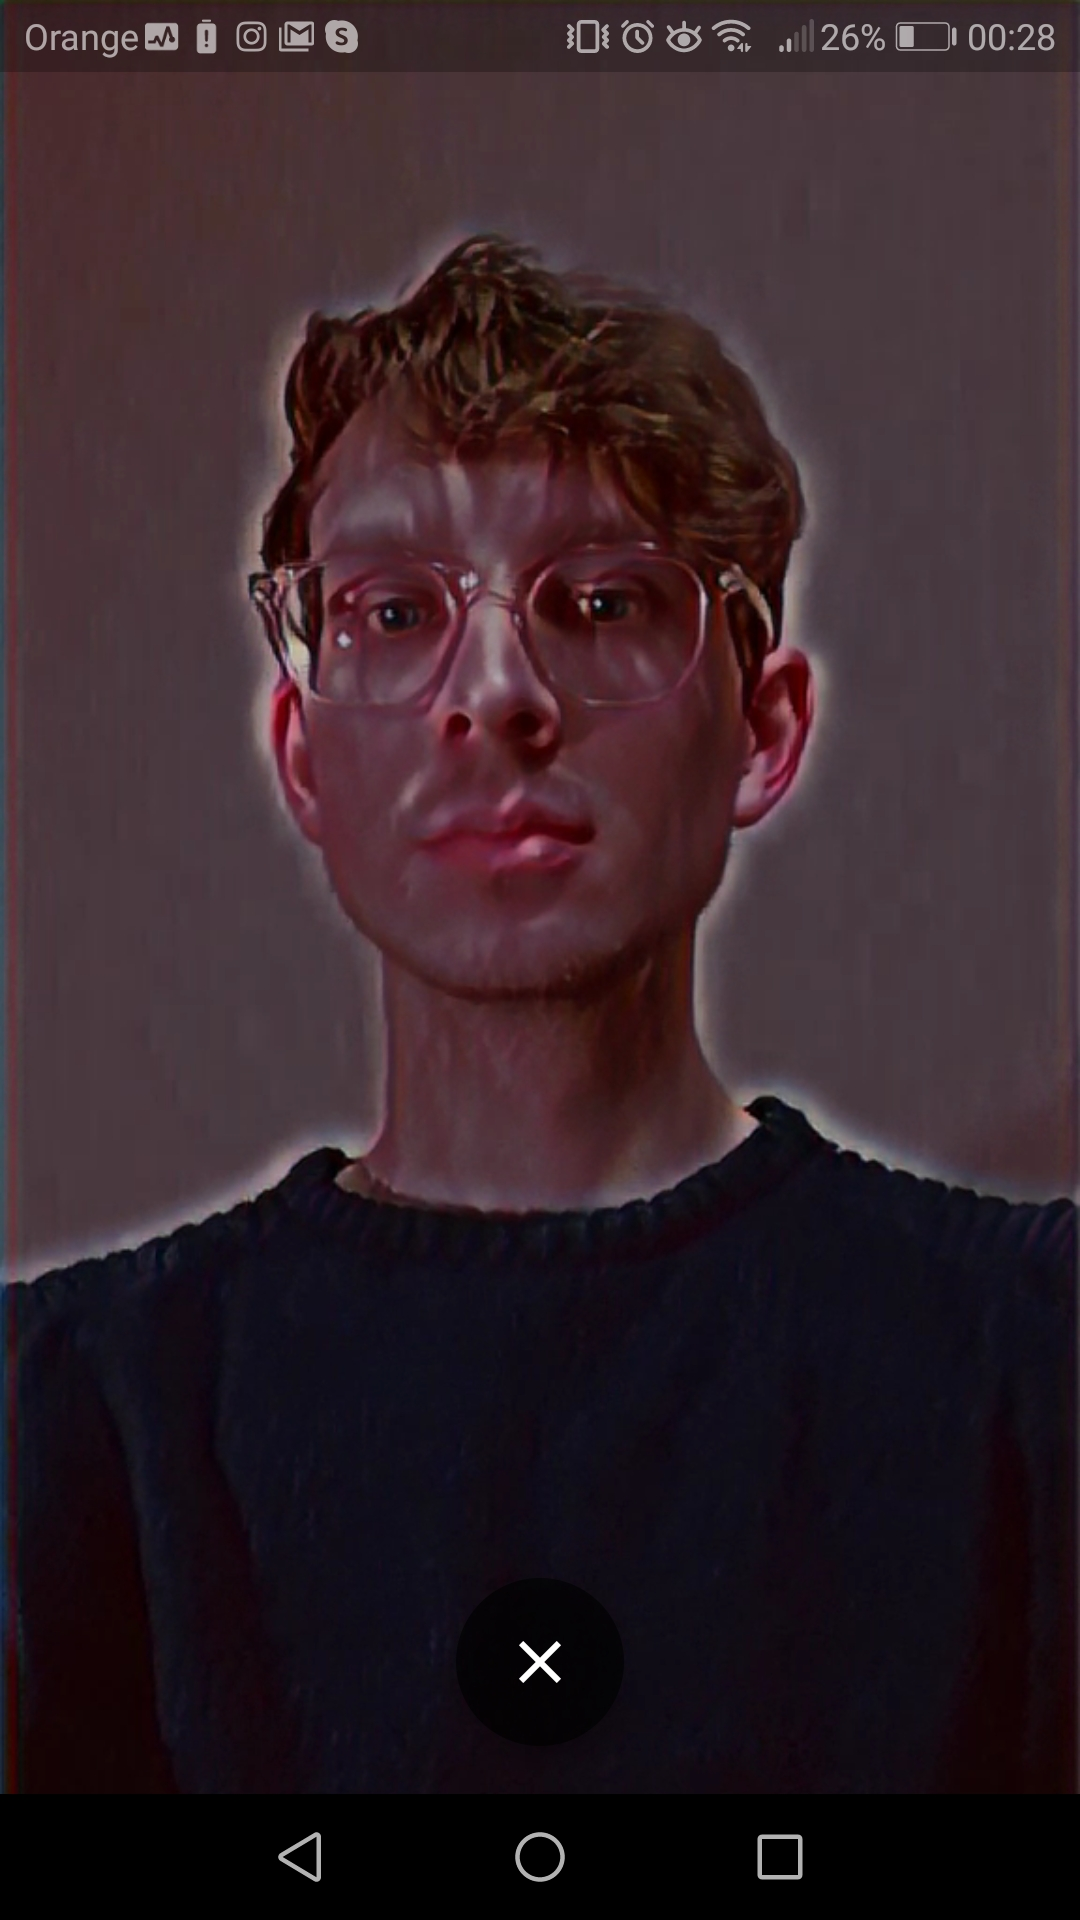
\includegraphics[width = 0.13\linewidth]{Images/app_photos/me/lets.jpg} &
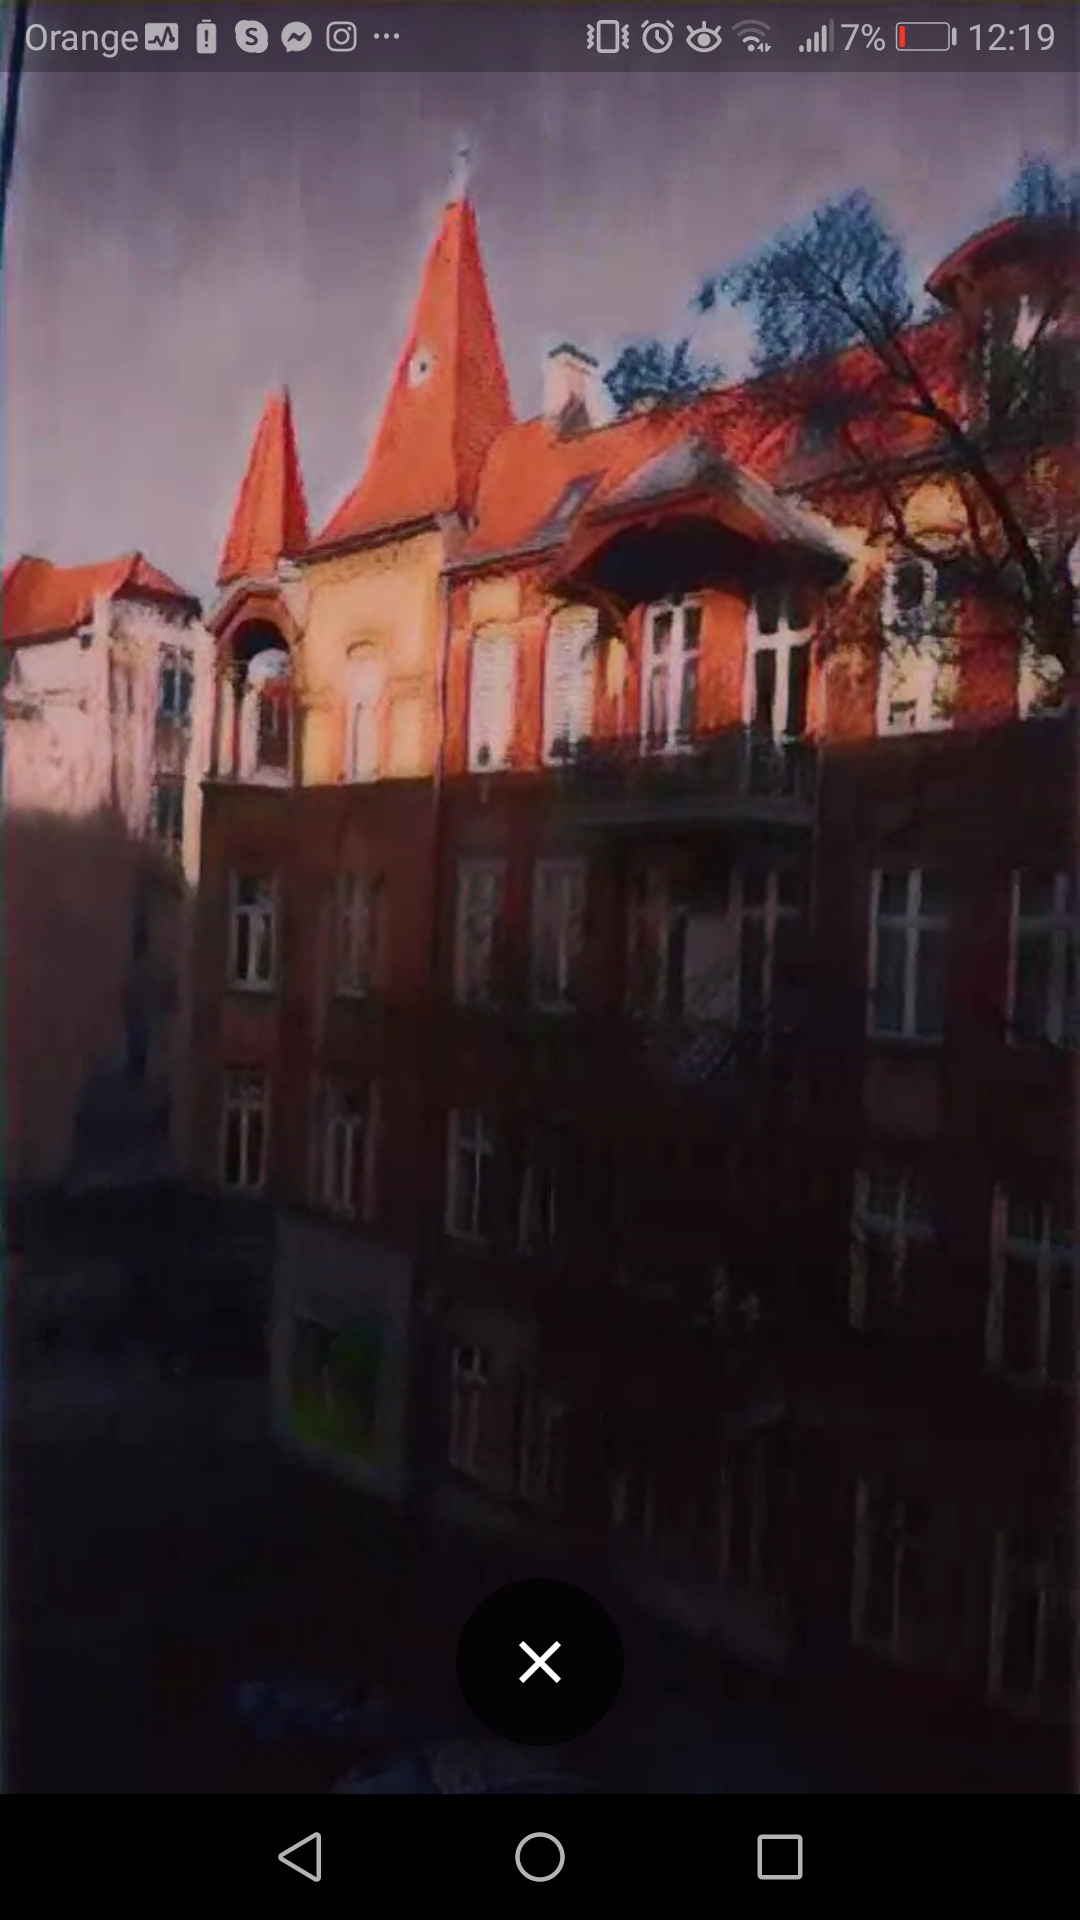
\includegraphics[width = 0.13\linewidth]{Images/app_photos/kamienica/lets.jpg} &
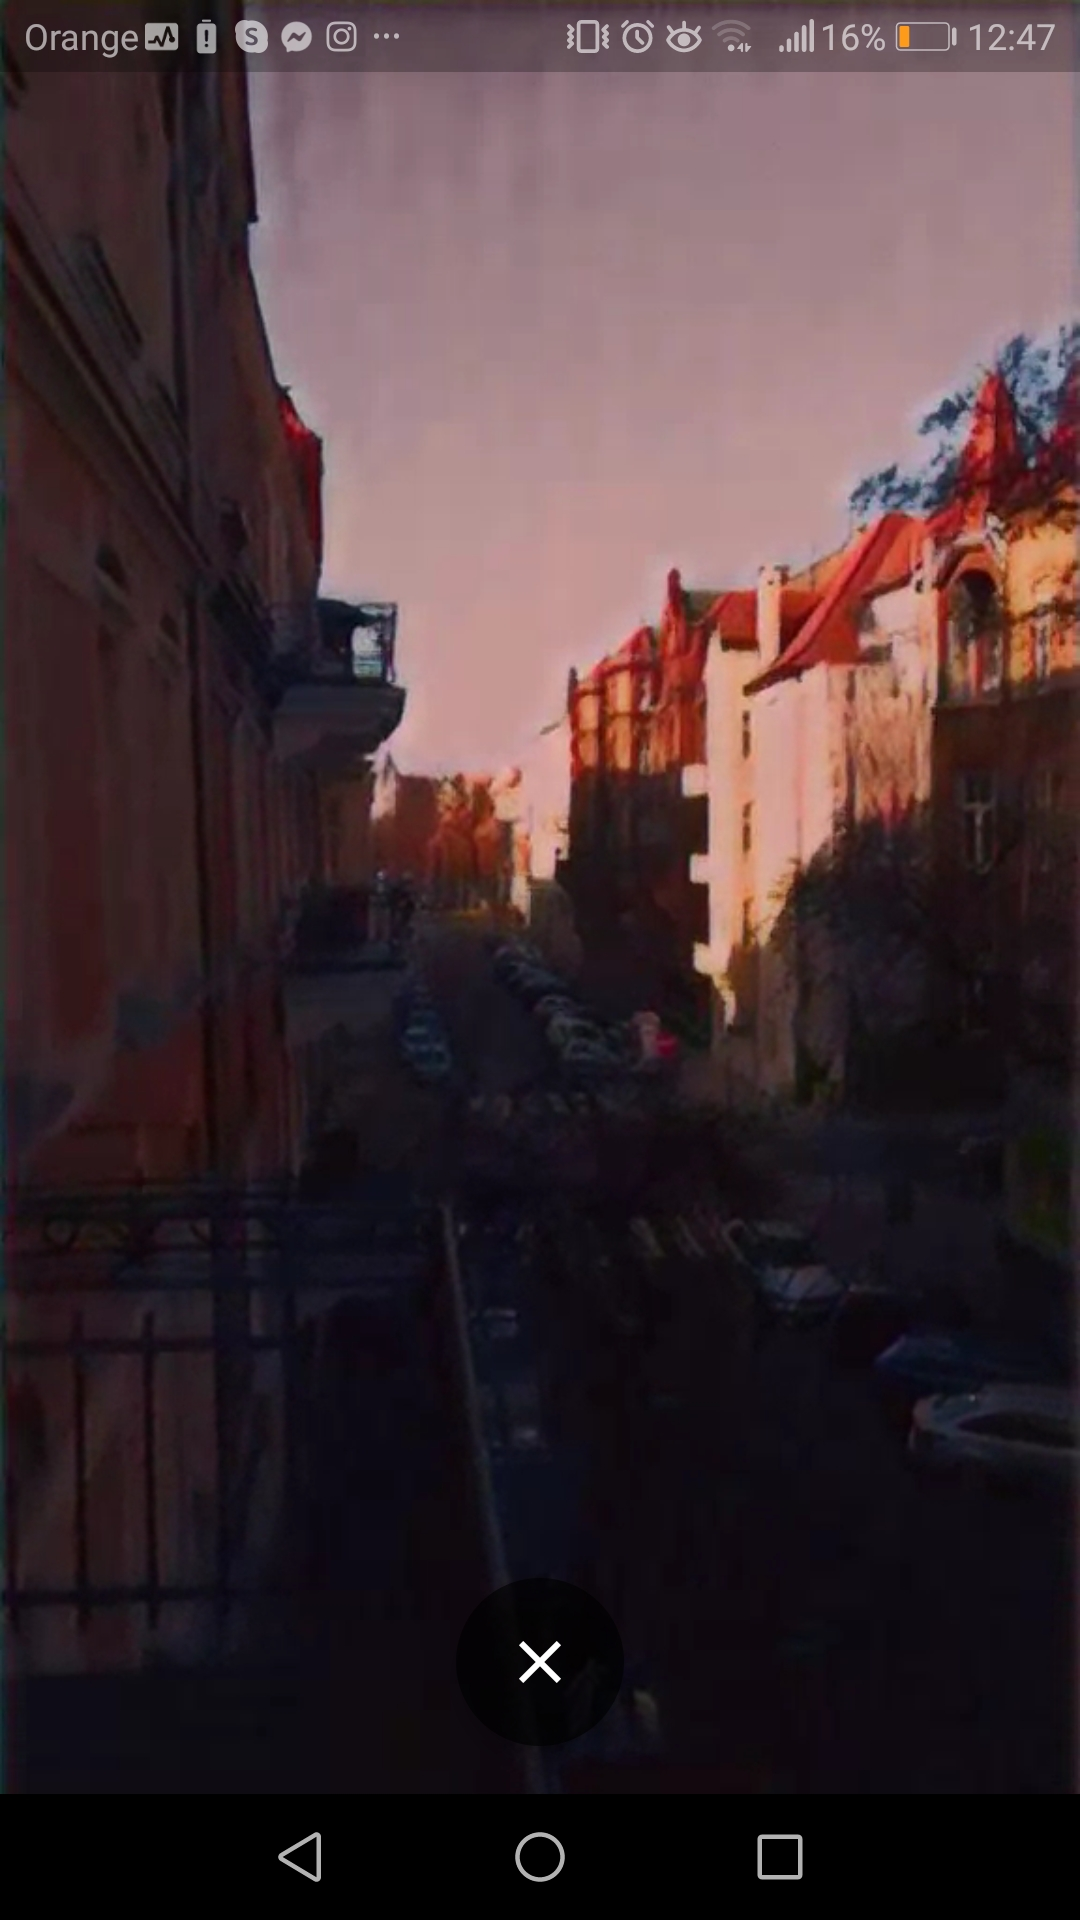
\includegraphics[width = 0.13\linewidth]{Images/app_photos/ulica/lets.jpg} \\

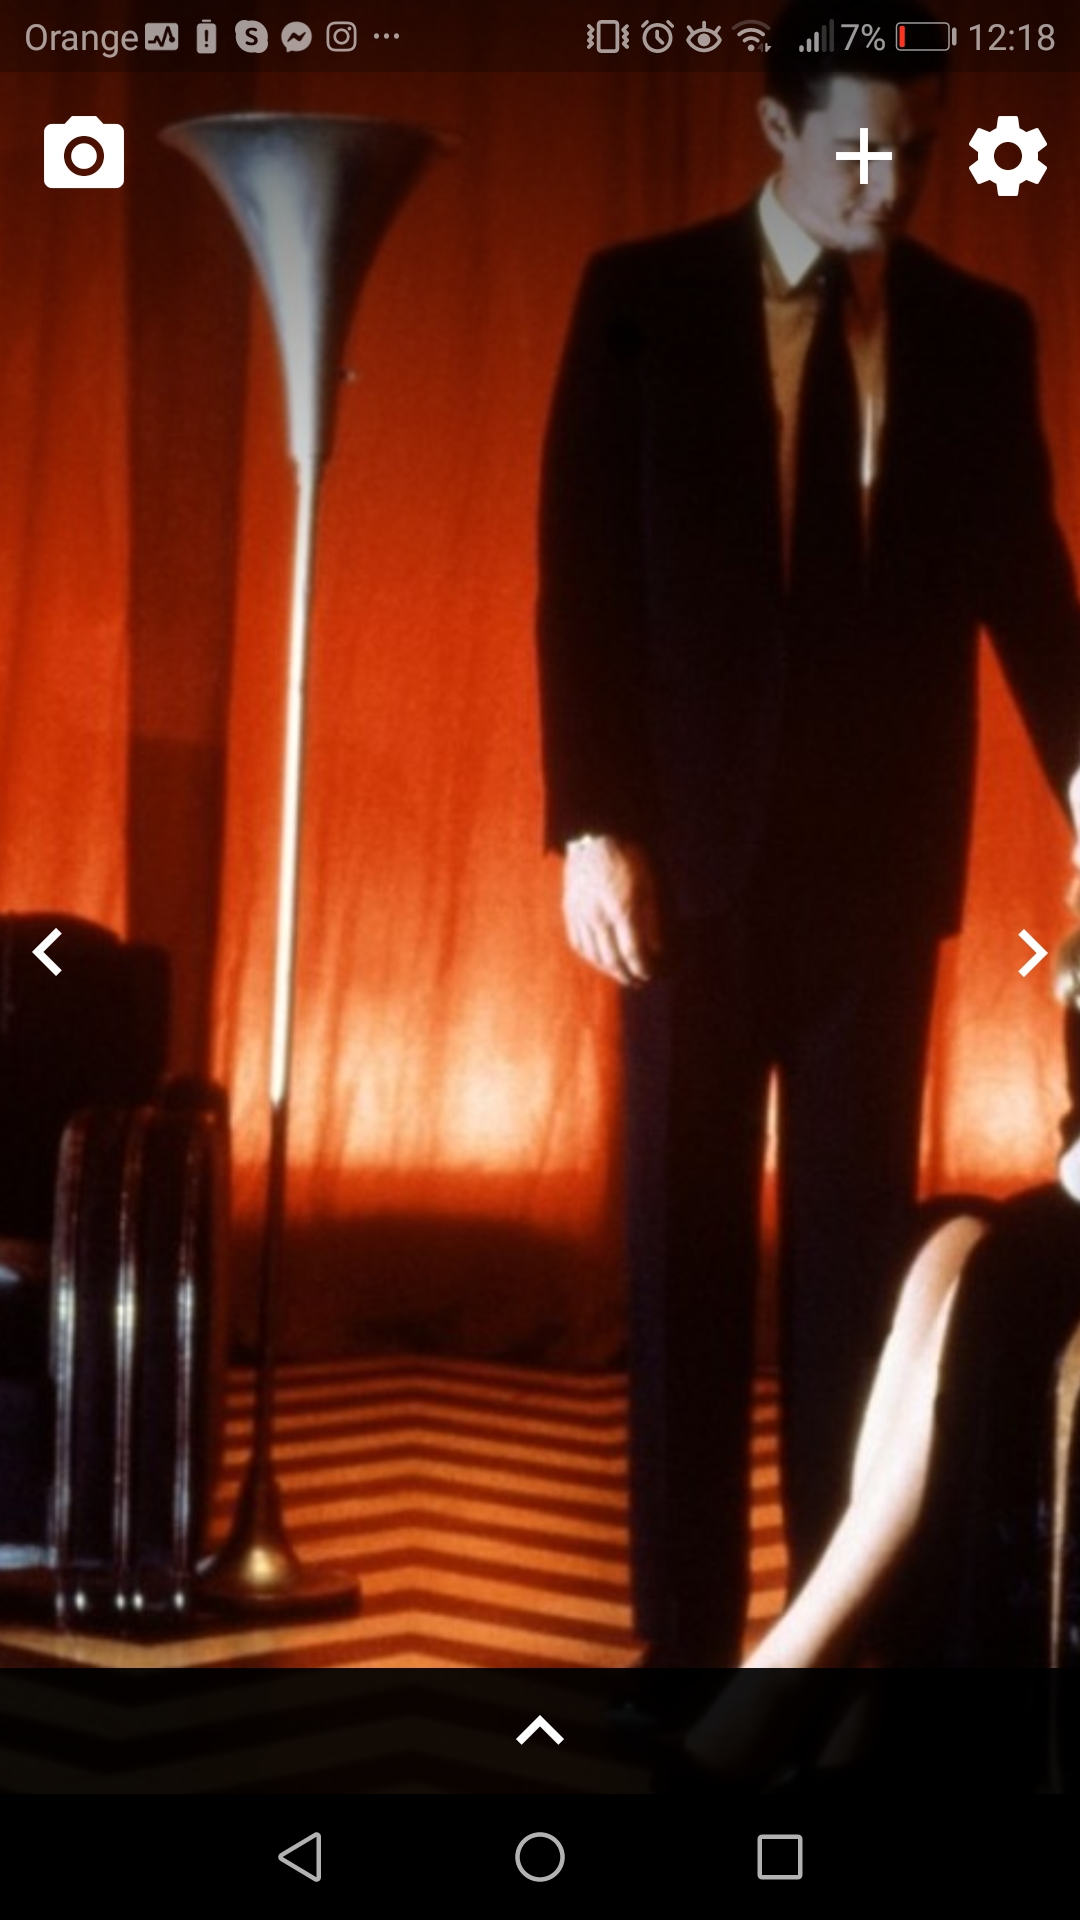
\includegraphics[width = 0.13\linewidth]{Images/app_photos/filters/twin.jpg} &
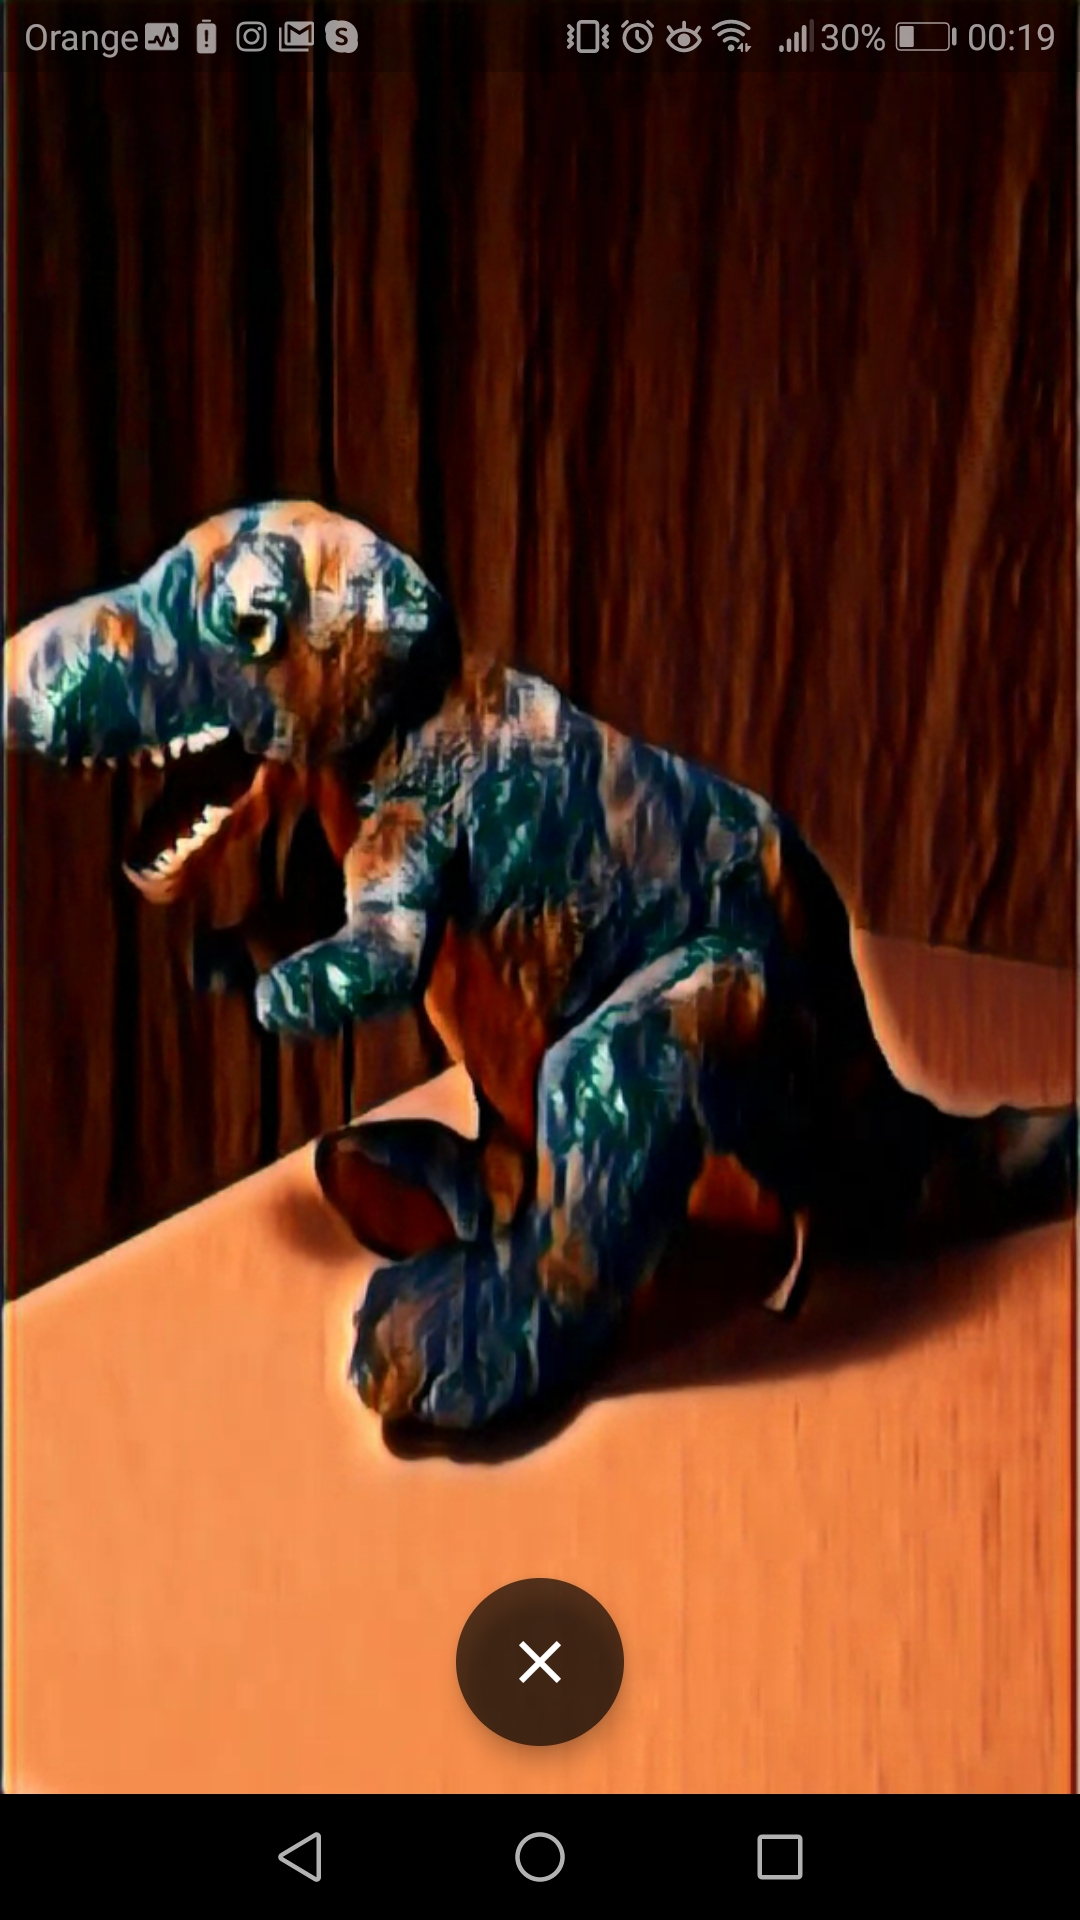
\includegraphics[width = 0.13\linewidth]{Images/app_photos/dino/twin.jpg} &
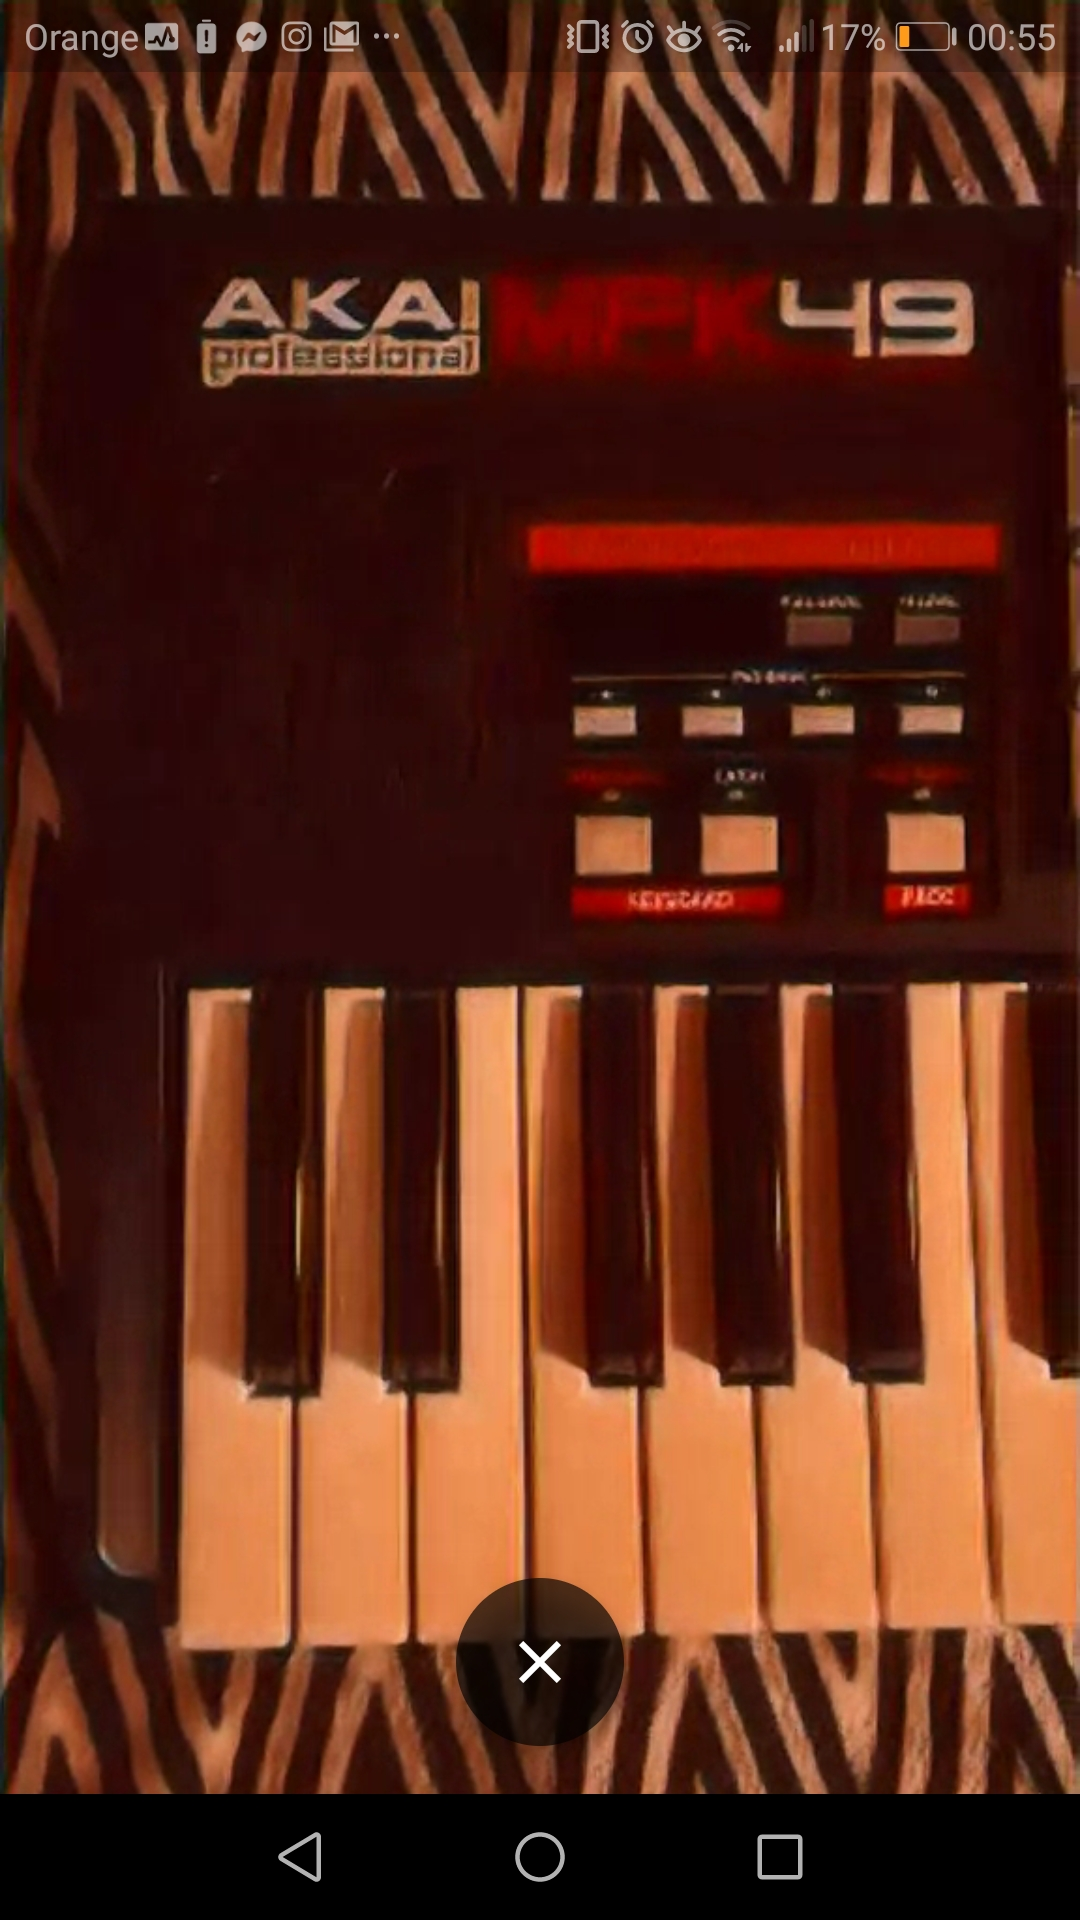
\includegraphics[width = 0.13\linewidth]{Images/app_photos/akai/twin.jpg} &
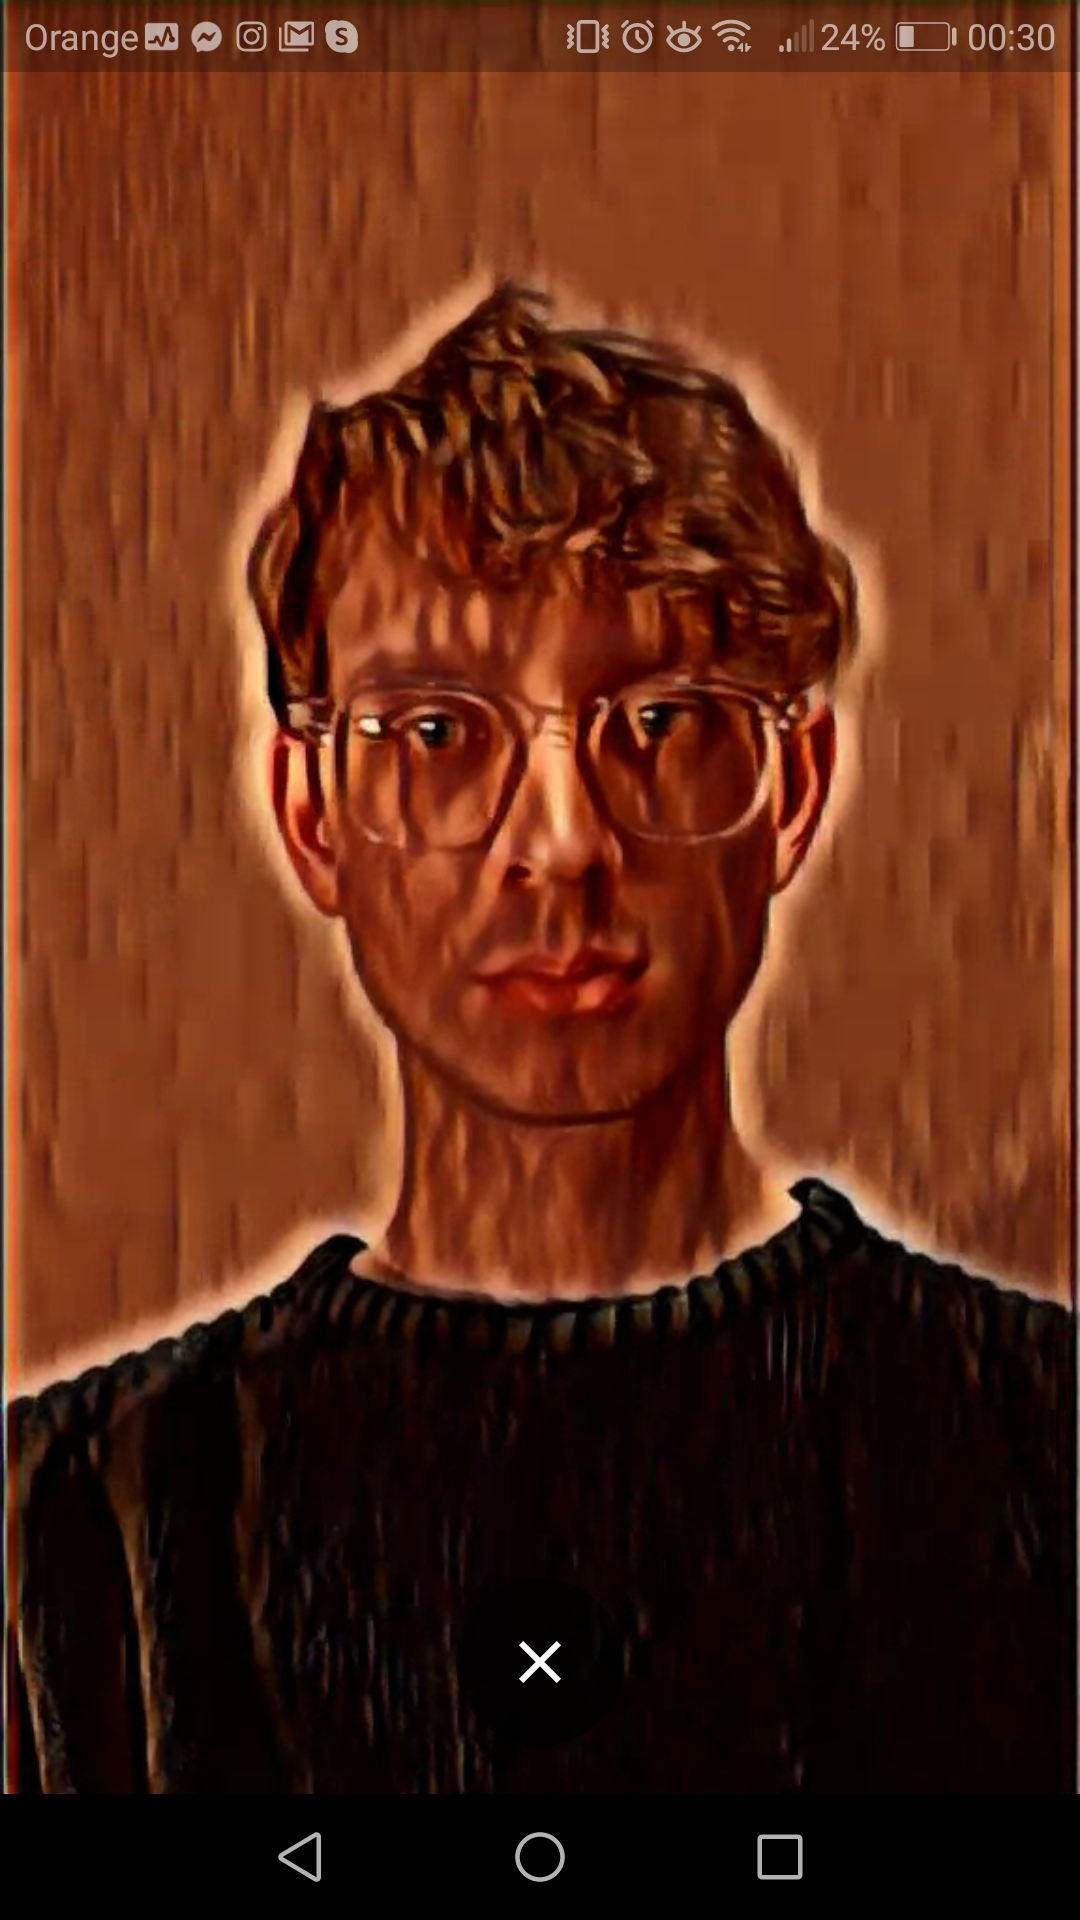
\includegraphics[width = 0.13\linewidth]{Images/app_photos/me/twin.jpg} &
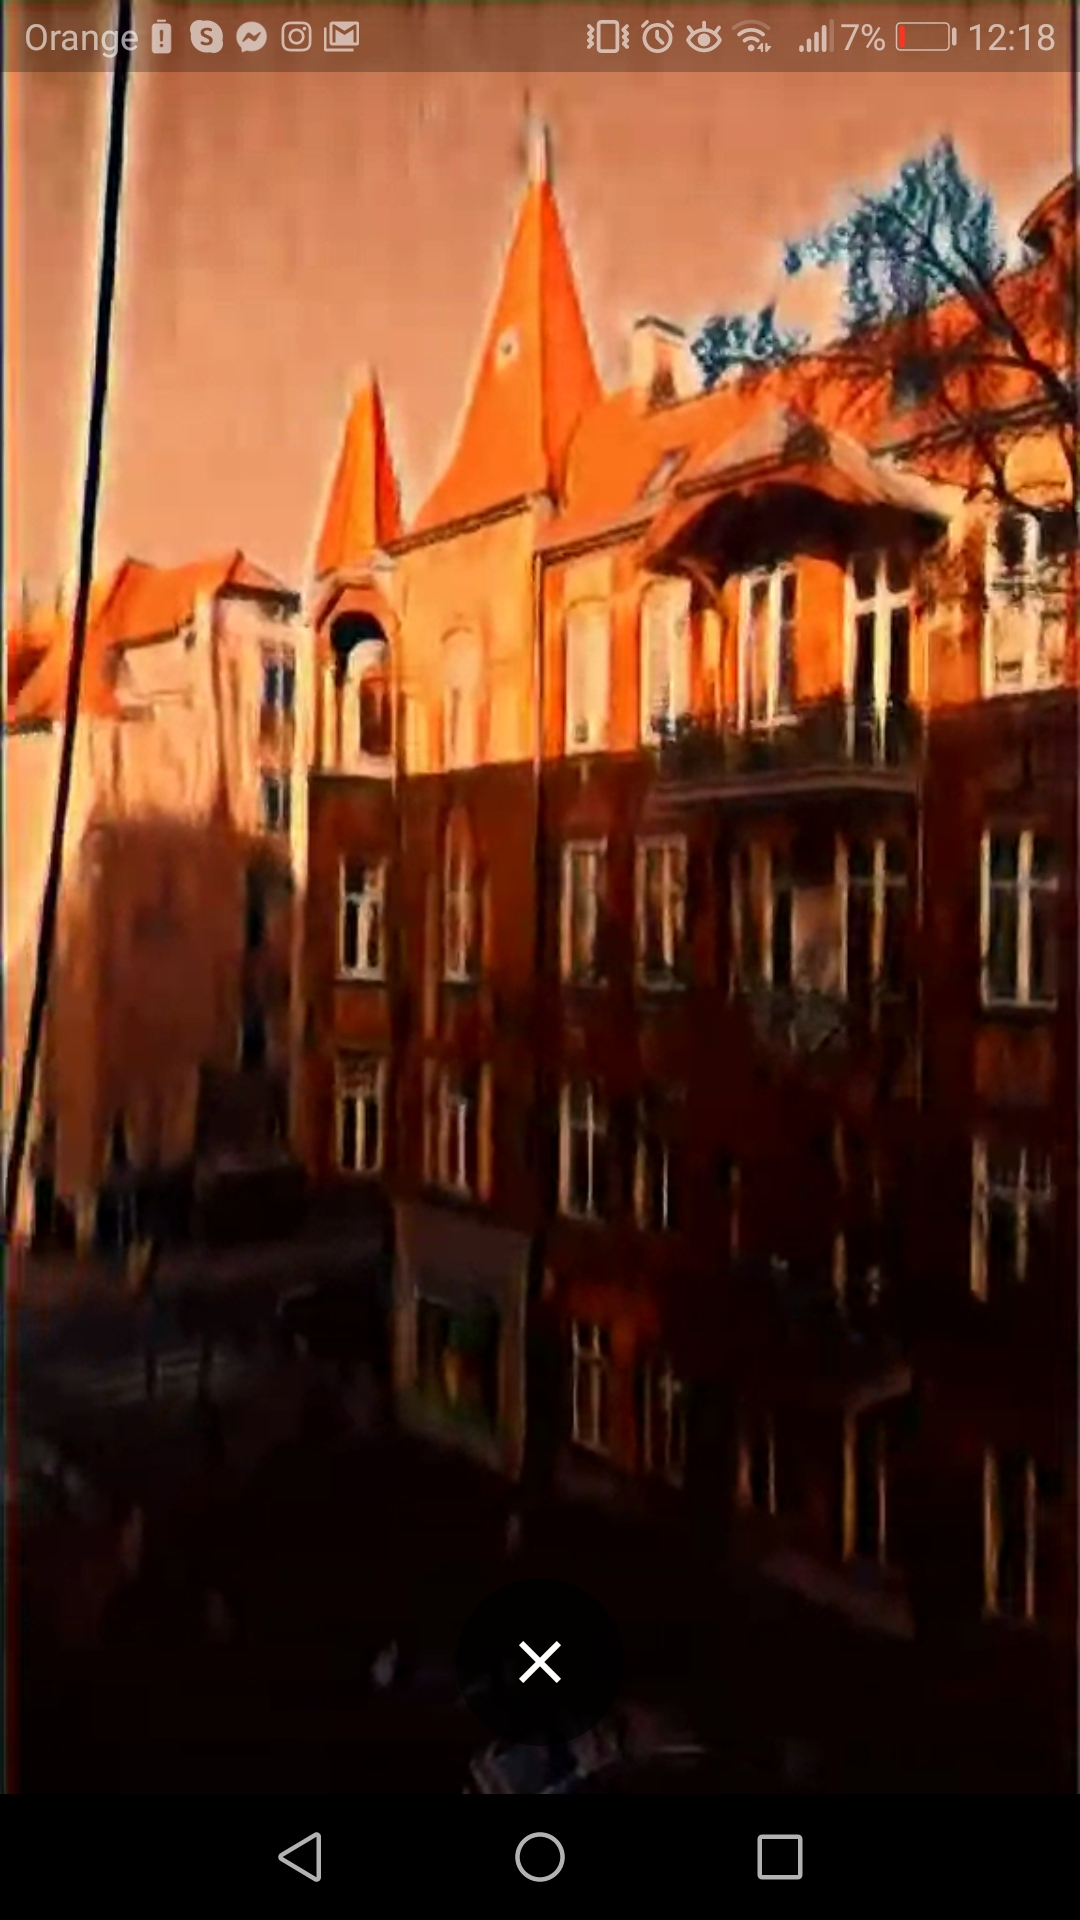
\includegraphics[width = 0.13\linewidth]{Images/app_photos/kamienica/twin.jpg} &
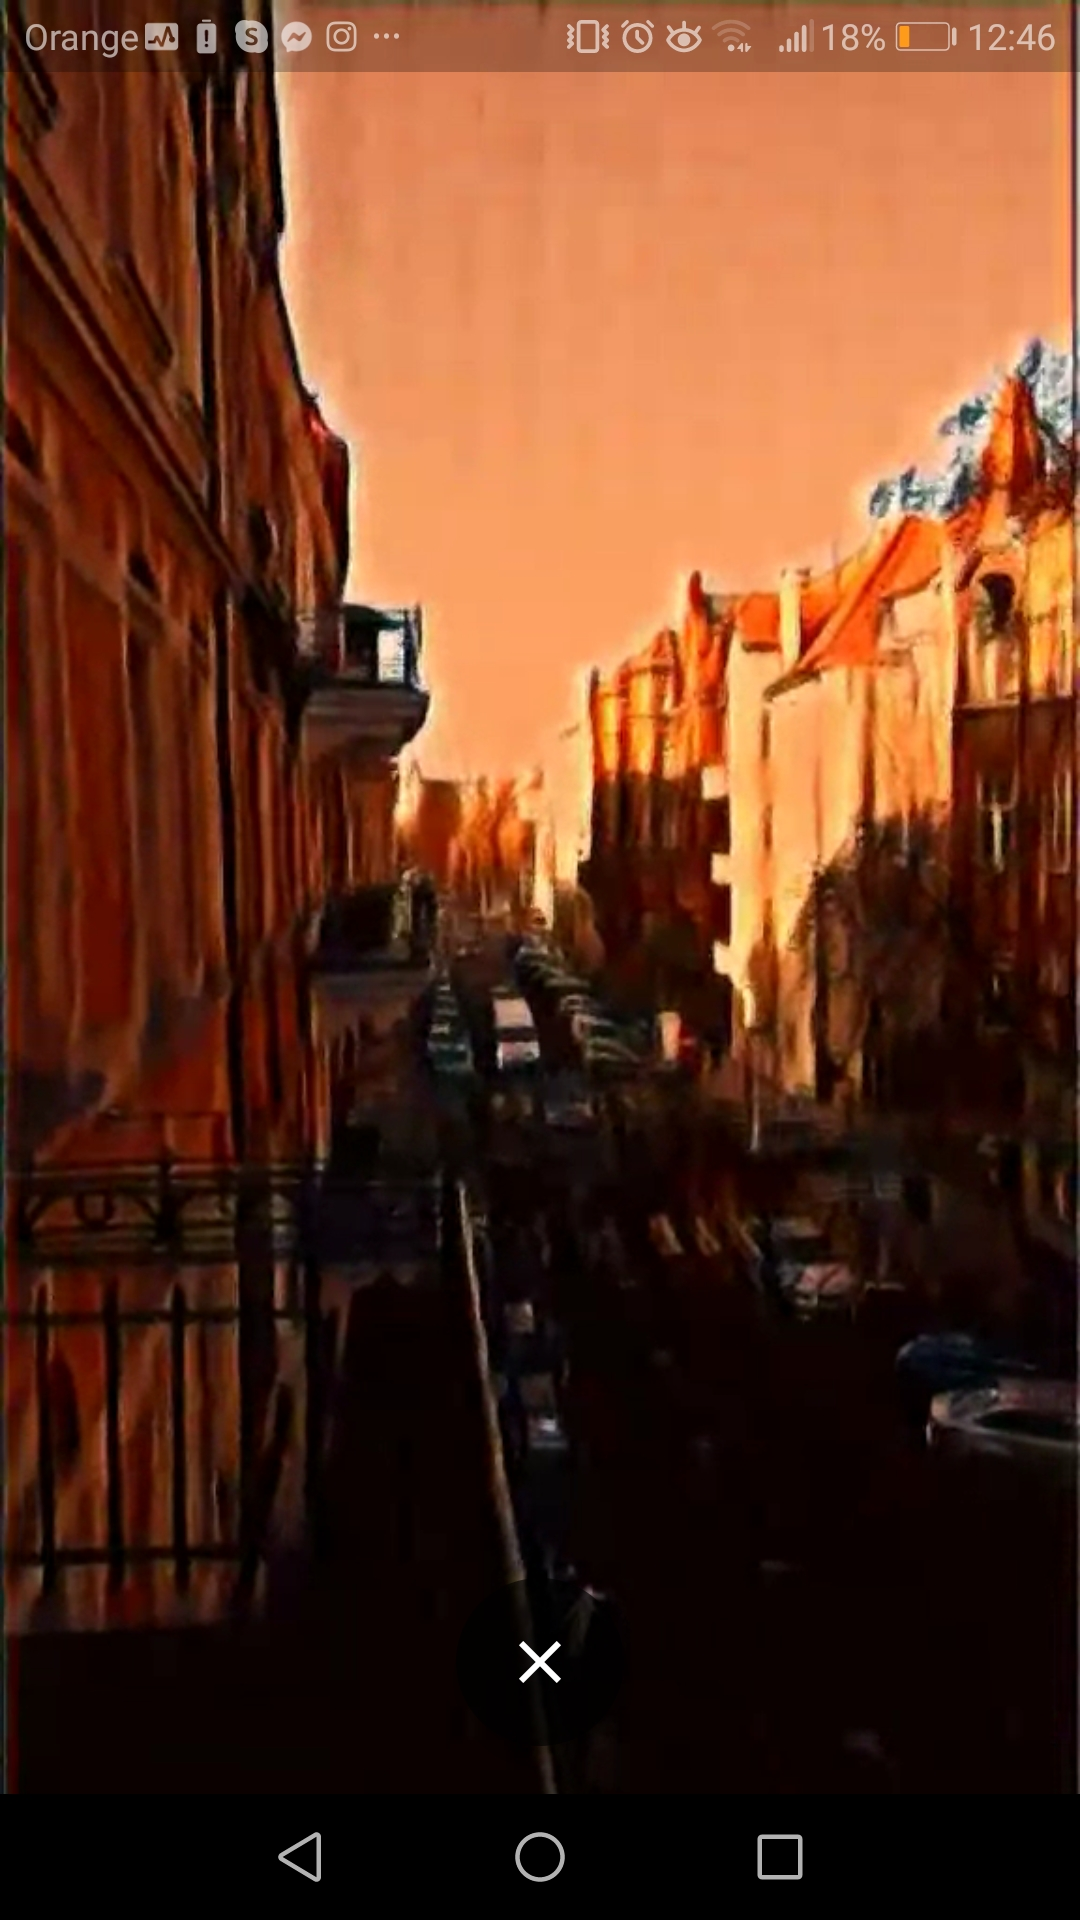
\includegraphics[width = 0.13\linewidth]{Images/app_photos/ulica/twin.jpg} \\


\includegraphics[width = 0.13\linewidth]{Images/app_photos/filters/under.jpg} &
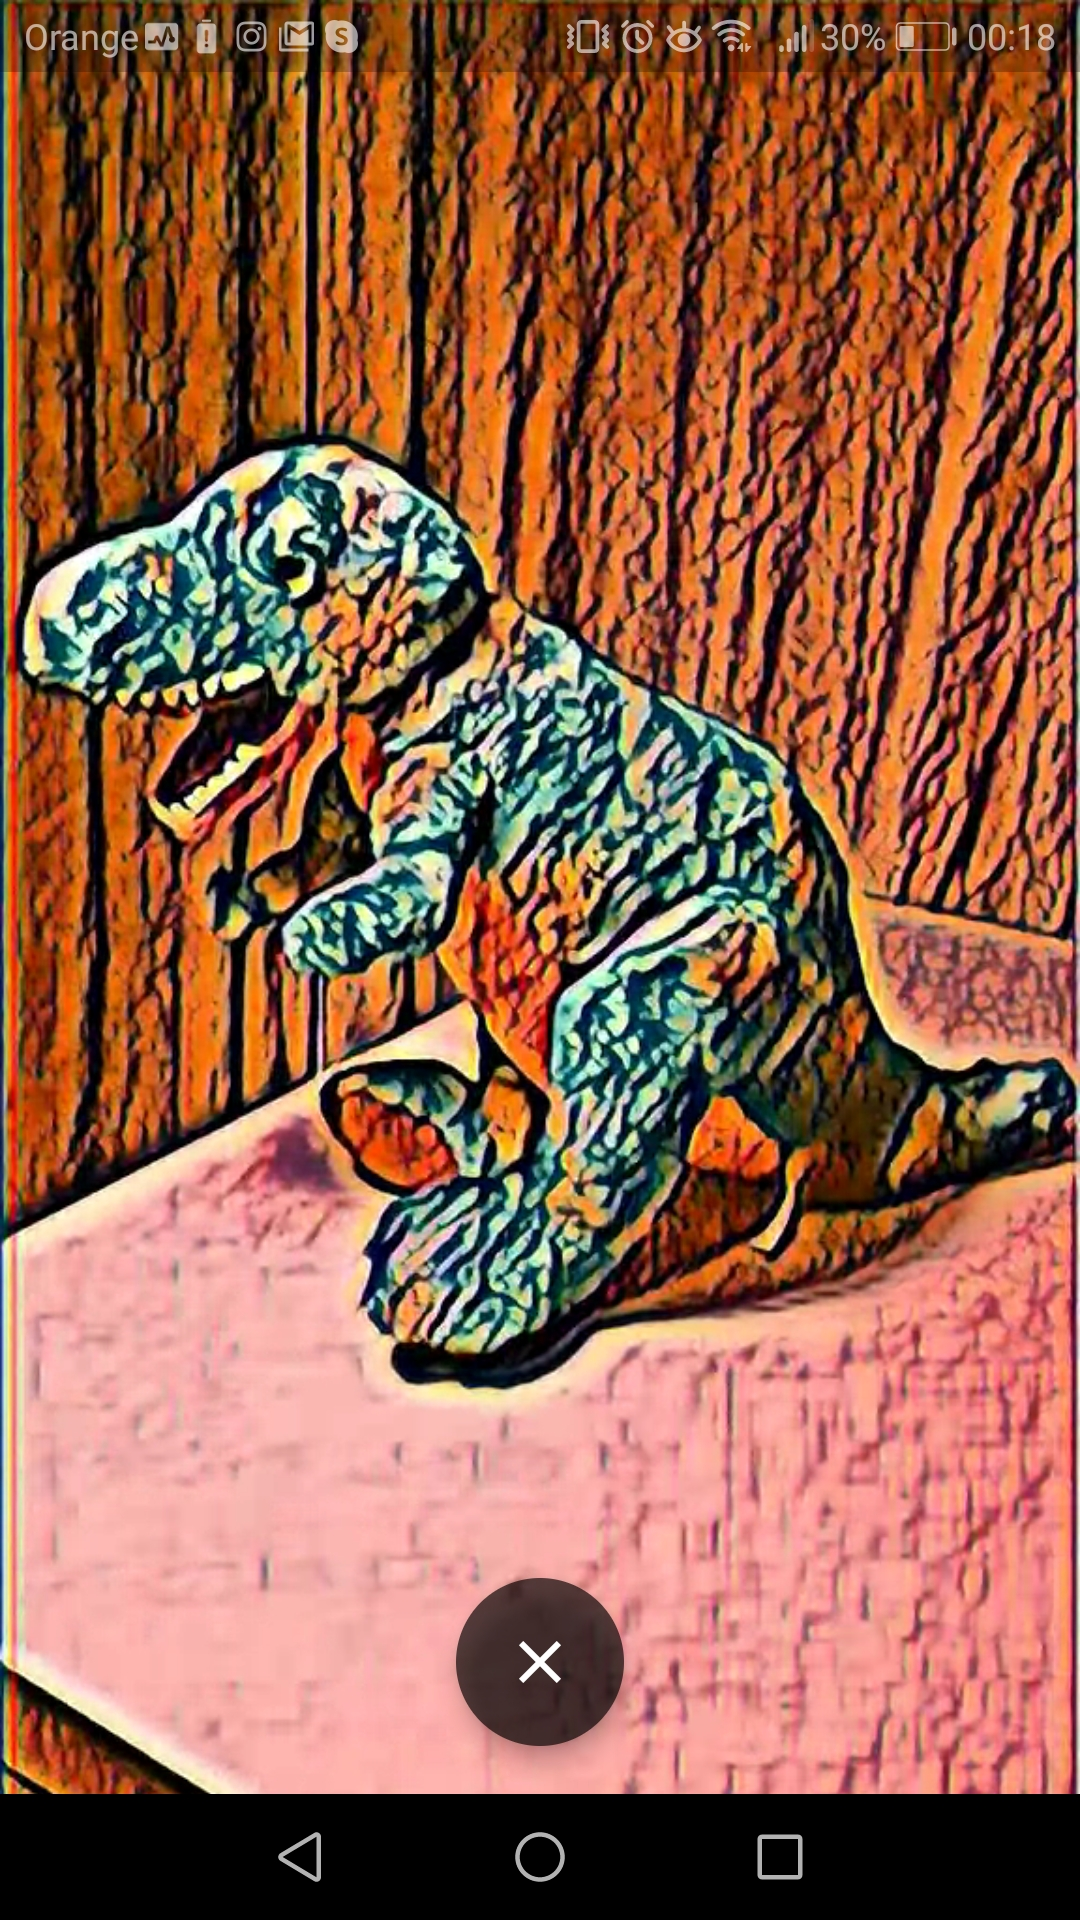
\includegraphics[width = 0.13\linewidth]{Images/app_photos/dino/under.jpg} &
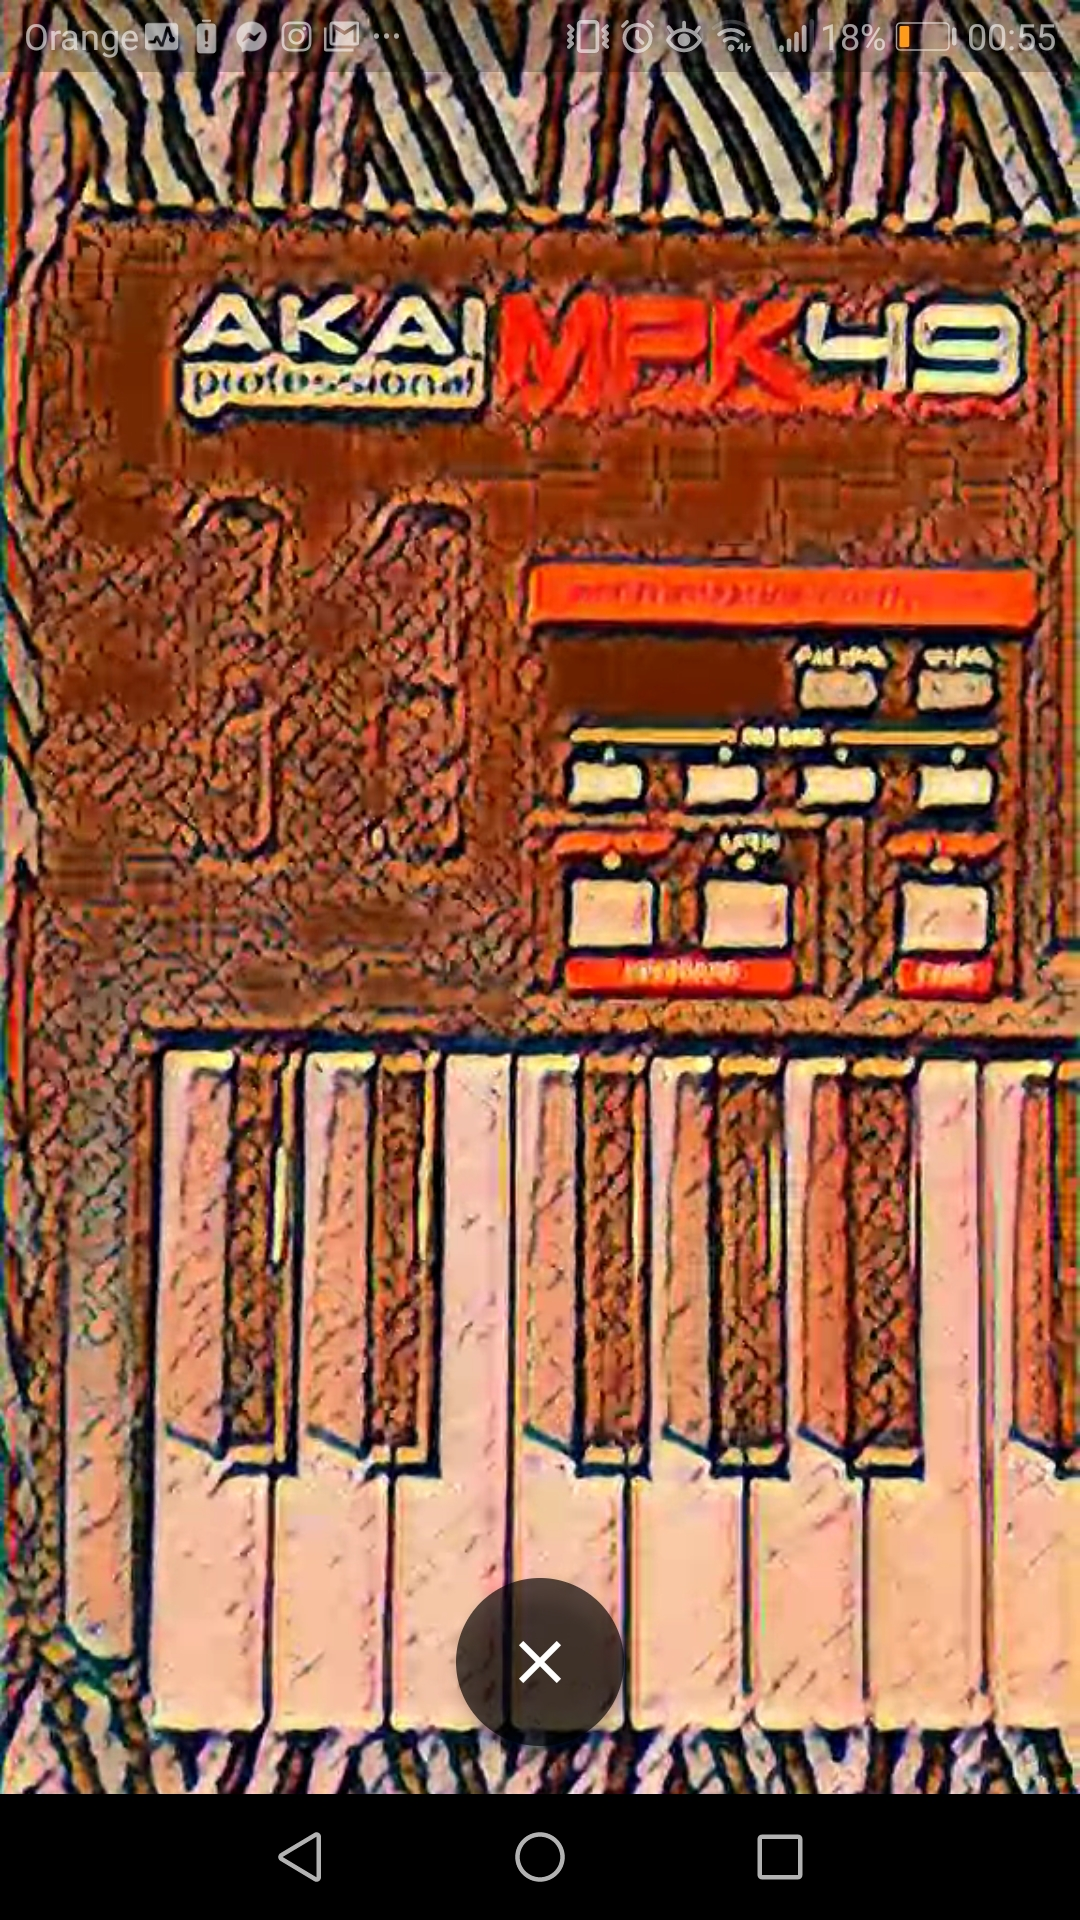
\includegraphics[width = 0.13\linewidth]{Images/app_photos/akai/under.jpg} &
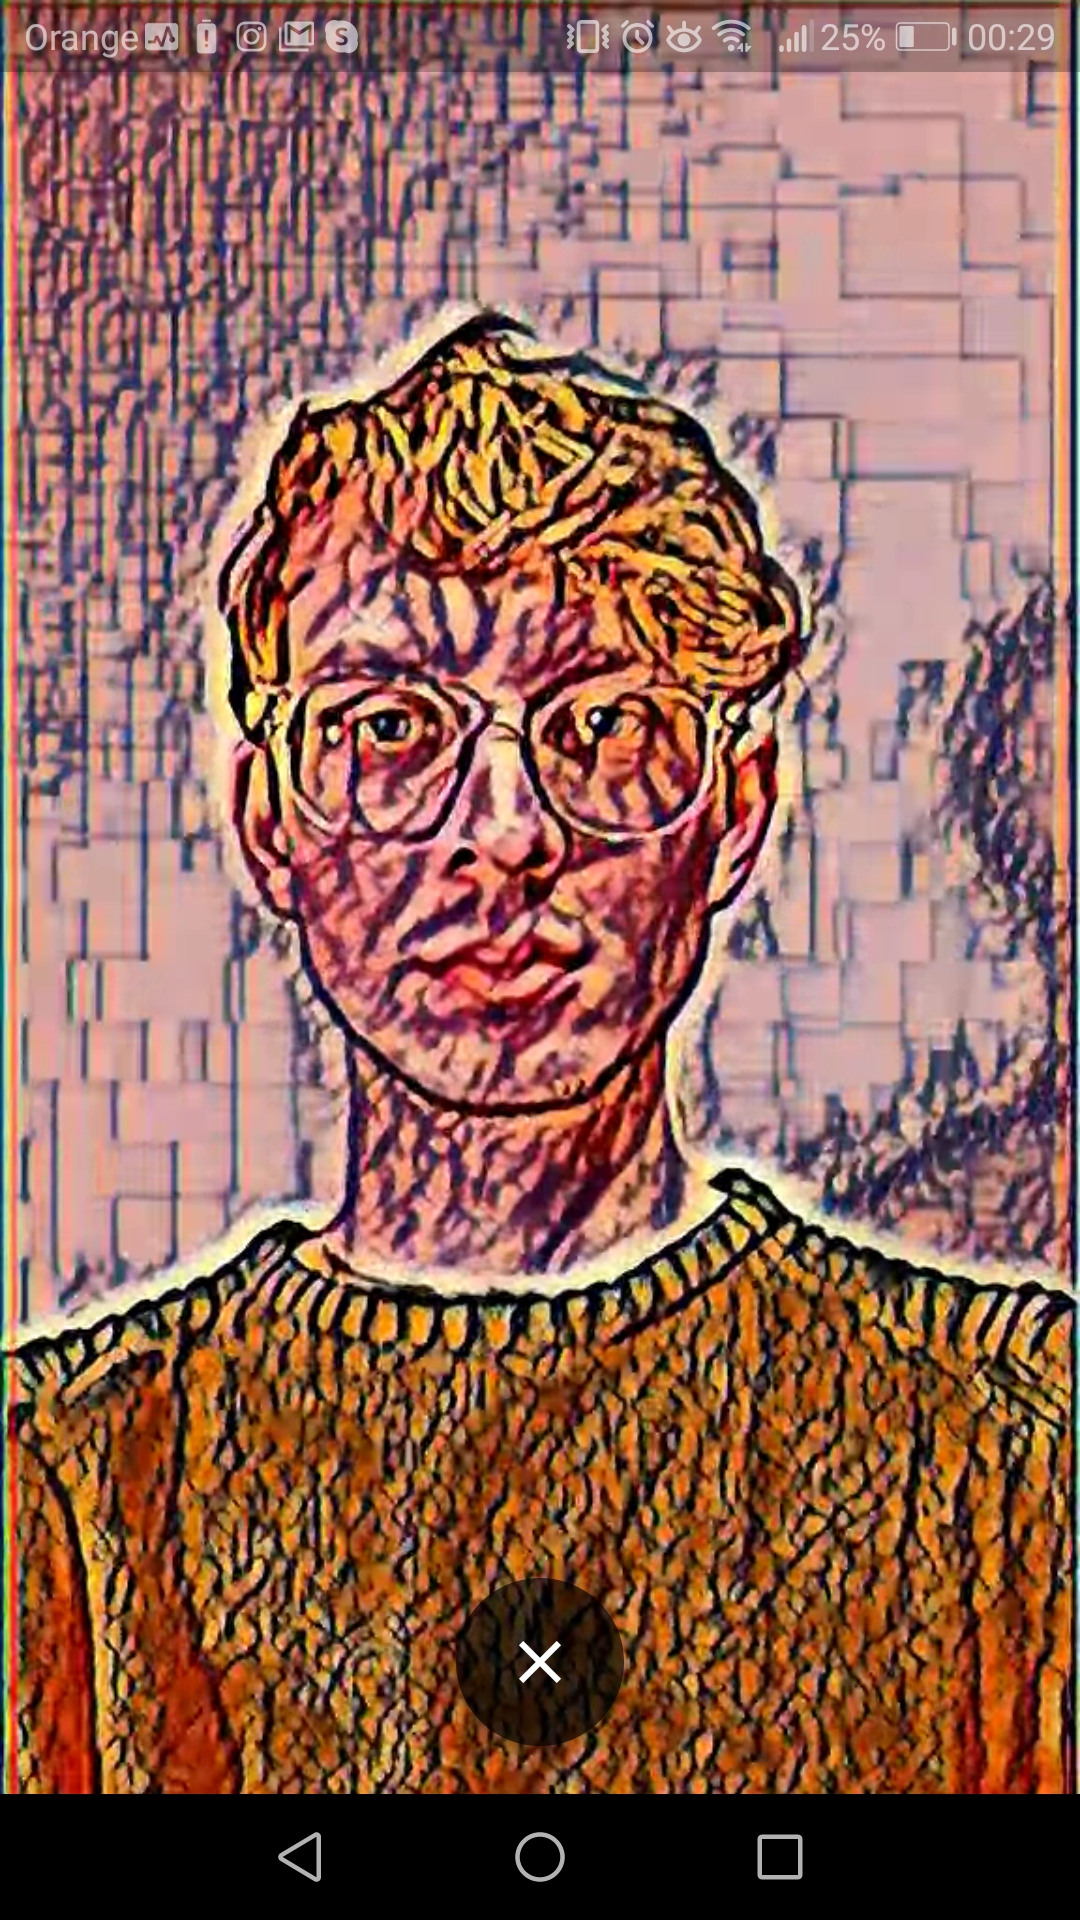
\includegraphics[width = 0.13\linewidth]{Images/app_photos/me/under.jpg} &
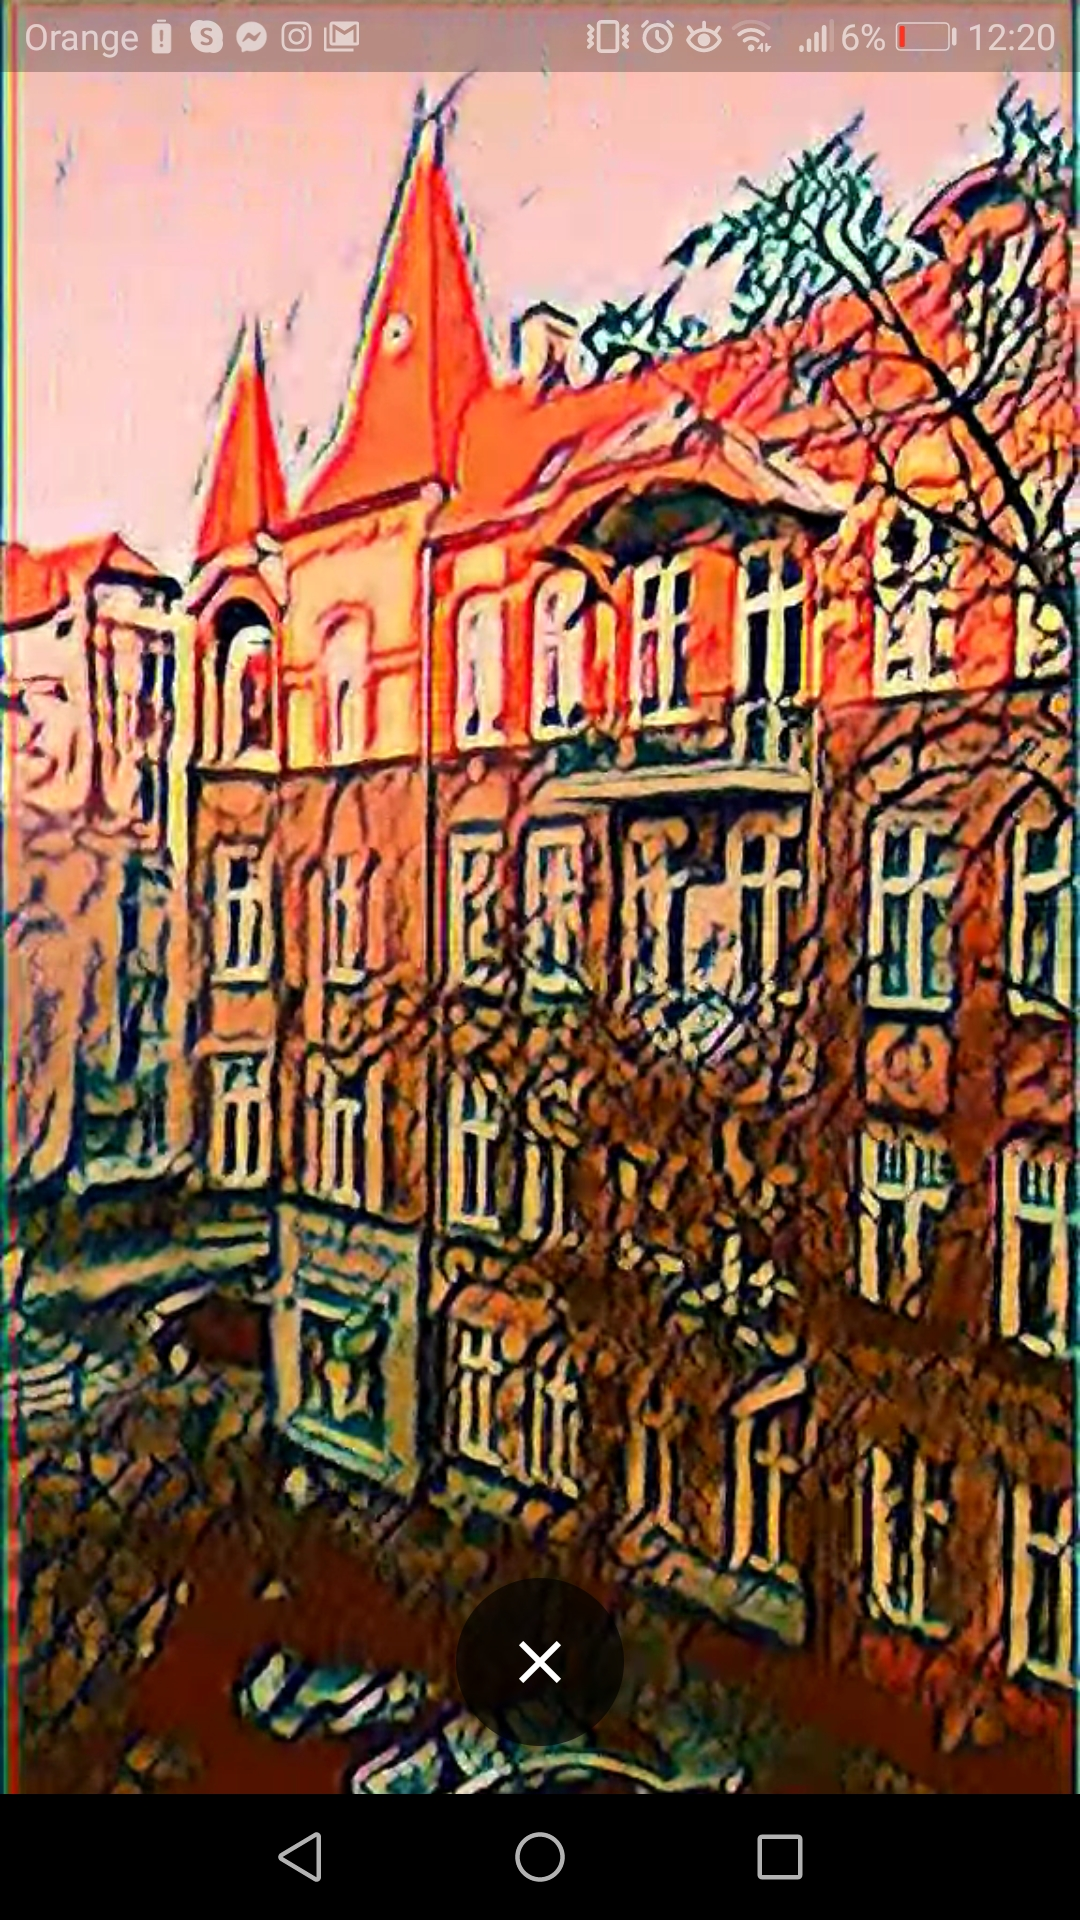
\includegraphics[width = 0.13\linewidth]{Images/app_photos/kamienica/under.jpg} &
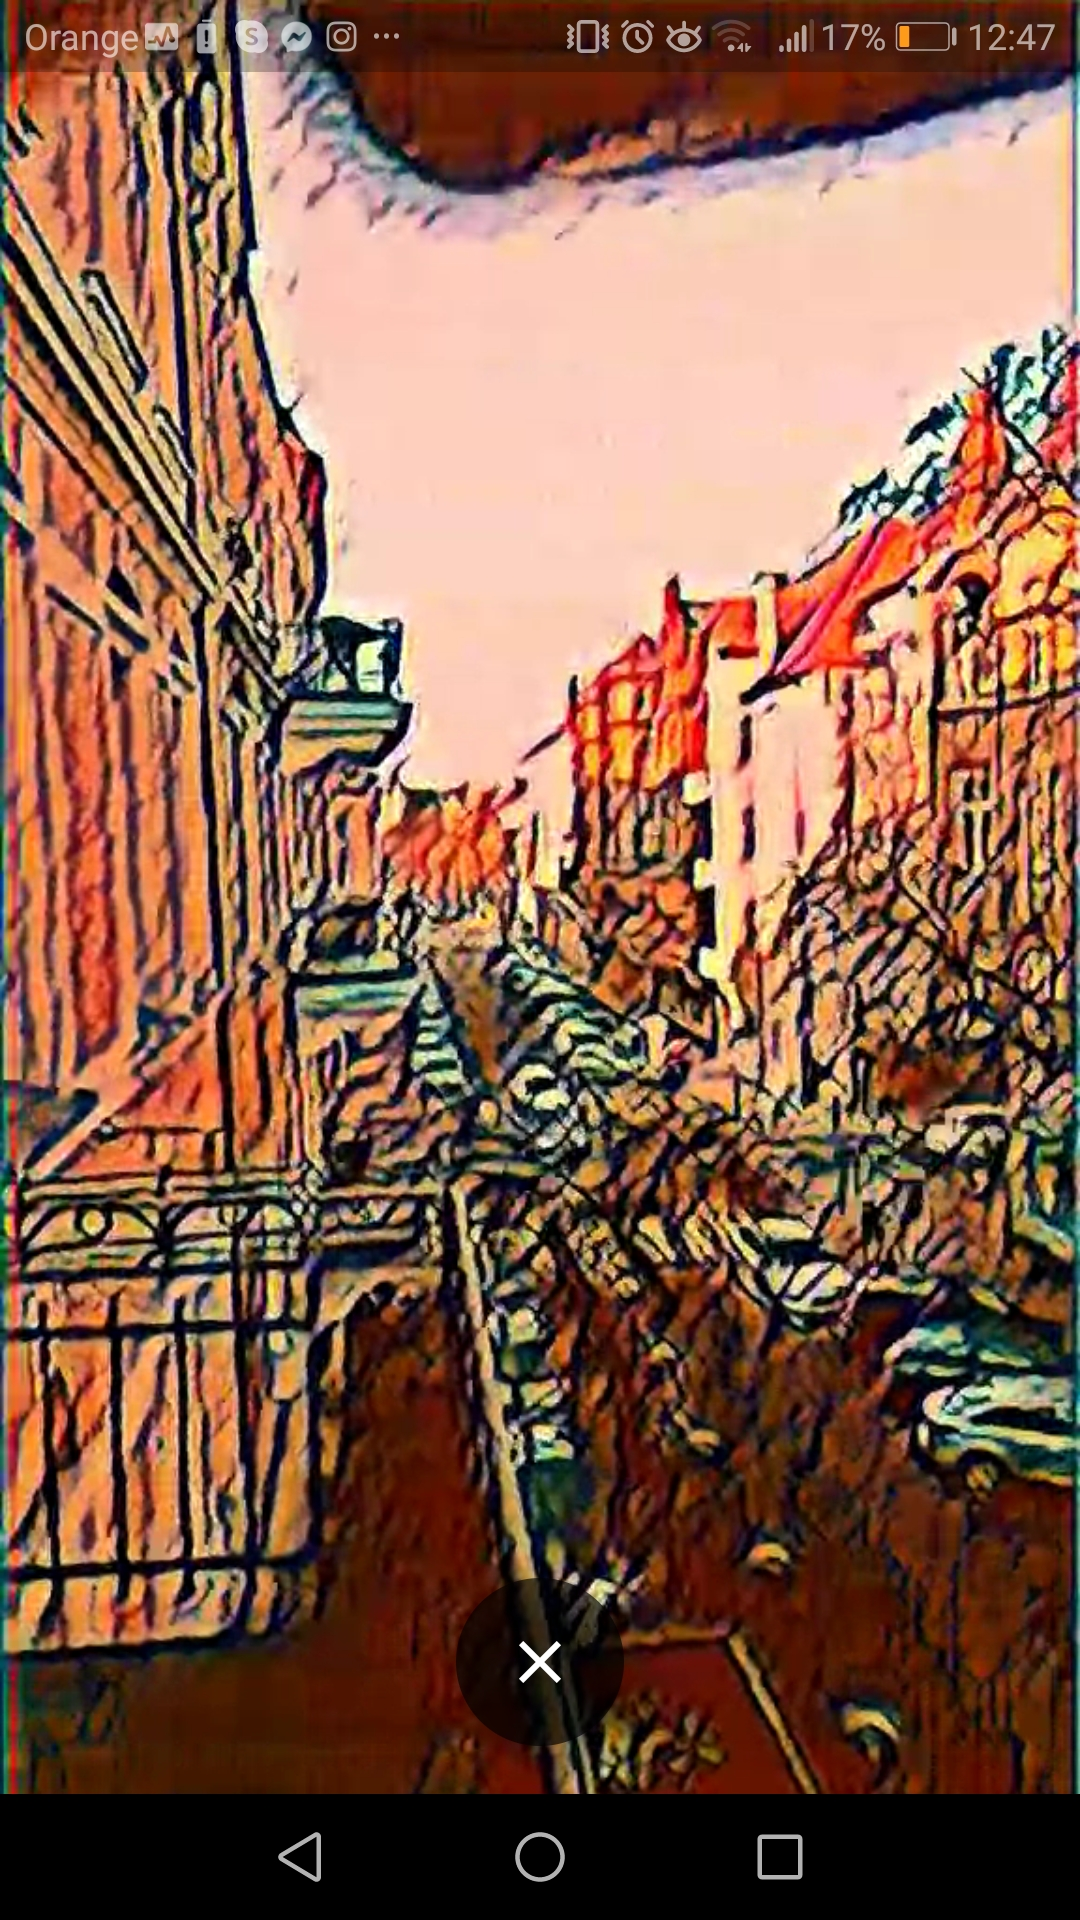
\includegraphics[width = 0.13\linewidth]{Images/app_photos/ulica/under.jpg} \\

\end{tabular}
\caption{Style transfer in mobile application}
\label{fig:app-results}
\end{figure}


\subsection{Future Works}
In this section we outline ideas and development directions we found interesting
throughout the development of this project.
\begin{itemize}
\item \textbf{Feature encoding}
    To construct encoder \cite{Li2018} train VGG-like architecrture to classify 
    MSCOCO images. While dataset is rather large (80000 images), training classifier
    is probably the simplest way to obtain deep extractor of meaningful image features.
    Training encoder to perform other, more demanding, computer vision tasks like 
    segmentation or image tagging might result in more robust features better suited
    for style transform. It would be particularly intersting to examine wheter use of encoders
    trained in unsupervised manner (e.g. \cite{CPC, CPCv2}) would make any difference.
    Such models need to be able to perform tasks demanding even for humans, like generating
    full image based on only a port of it. As a side effect representations produced by their
    encoders must contain useful information for range of computer vision tasks.
    Even if it didn't influence network's output, the it might perhaps ease the training
    and accelarate convergance of style transform models
\item \textbf{More sophisticated training}
    Image classification is a well-defined task with clear metric.
    Because of this simplicity, papers introducing new pruning algorithms tend to 
    benchmark performance on classifiers. As a result methods for efficient pruning of
    picture to picture models were not studied so thoroughly. Expanding loss function used during
    retraining of pruned network by some form of knowledge distillation might enable
    even more severe pruning of such models. One might for example penalize $\ell_2$
    distance between outputs of network being pruned and original network.
    This would help shorten retraining phase since $\ell_2$ gradient
    would be very large right after removal of some filters and quickly steer pruned
    model's parameters towards original.
    
    
\end{itemize}

\biblio % Needed for referencing to working when compiling individual subfiles - Do not remove
\end{document}
